\documentclass{beamer}
%\usetheme{Madrid}
\usecolortheme{iwr}

\usepackage[utf8]{inputenc}
\usepackage[german]{babel}
\usepackage{url}
\usepackage{nicefrac}
%\usepackage[export]{adjustbox} % Used for vertical alignment of tikz images, but failed
\usepackage{graphicx}
\usepackage{tikz,tikzscale}
\usepackage{pgfplots}
\pgfplotsset{compat=1.18}
\usetikzlibrary{arrows.meta,calc}
\usepackage{amsthm}
\usepackage{float}
\usepackage{environ}
\usepackage{listings}
\lstset{language=Matlab}


\title{Mathematik für Molekulare Biotechnologie B}
\author{Guido Kanschat}
\date{Fakultät für Ingenieurwissenschaften\\Universität Heidelberg}

\usepackage[mode=multiuser]{fixme}
%\fxsetup{innerlayout=inline}
%\fxsetup{targetlayout=colorcb}
\fxusetheme{color}
\FXRegisterAuthor{gk}{envgk}{GK}
\FXRegisterAuthor{mr}{envmr}{MR}

\theoremstyle{remark}
\newenvironment{Aufgabe}{\begin{onlyenv}<article>\subsubsection{Aufgabe}}{\end{onlyenv}}
\newenvironment{Wdh}{\begin{onlyenv}<article>\textbf{Wiederholung: }}%
{\end{onlyenv}}
\newenvironment{Vertiefung}{\begin{onlyenv}<article>\textbf{Vertiefung: }}%
{\end{onlyenv}}
\newenvironment{Denkpause}{%
  \begin{onlyenv}<presentation>%
    \begin{exampleblock}{Denkpause}%
}{%
    \end{exampleblock}%
  \end{onlyenv}%
}

\NewEnviron{Abschluss}{%
  \begin{frame}[label=Abschluss]
    \frametitle{Abschlussfragen \only<presentation>{\thesection.}\thesubsection}
    \begin{enumerate}
      \BODY
    \end{enumerate}%
  \end{frame}%
}

\let\epsilon\varepsilon
\let\phi\varphi
\let\theta\vartheta
\def\ii{\mathrm i}
\def\ds{\,ds}
\def\dt{\,dt}
\def\vecsym#1{\mathbf{#1}}
\def\vx{\vecsym x}
\def\vy{\vecsym y}
\def\vb{\vecsym b}
\def\vd{\vecsym d}
\def\ve{\vecsym e}
\def\vf{\vecsym f}
\def\vF{\vecsym F}
\def\vg{\vecsym g}
\def\vS{\vecsym S}
\def\vT{\vecsym T}
\def\vu{\vecsym u}
\def\vv{\vecsym v}
\def\vw{\vecsym w}
\def\R{\mathbb R}
\def\Rnn{\R^{n\times n}}

\def\norm#1{\left\|#1\right\|}
\def\scal(#1,#2){\left<#1,#2\right>}

\makeatletter
\@addtoreset{framenumber}{section}
\makeatother

\AtBeginSection[]{\frame<presentation>{\tableofcontents[currentsection,hideothersubsections]}}
\AtBeginSubsection[]{\frame<presentation>{\tableofcontents[sectionstyle=show/hide,subsectionstyle=show/shaded/hide]}}

\setbeamertemplate{navigation symbols}{}
\setbeamertemplate{section in toc}[sections numbered]
\setbeamertemplate{subsection in toc}[subsections numbered]
\setbeamertemplate{section in toc shaded}[default][50]
\setbeamertemplate{subsection in toc shaded}[default][50]
%\setbeamertemplate{footline}[frame number]
\setbeamertemplate{footline}{
  \hfill
  \insertsectionnumber/\insertframenumber
  \kern1em
  \vskip2pt
}


%\setcounter{section}{4}
%\makeatletter
%\beamer@tocsectionnumber=4 % TOC also starts from 3
%\makeatother

\begin{document}
\maketitle

\begin{frame}{Inhaltsübersicht}
   \tableofcontents[hideallsubsections]
\end{frame}

\includeonlyframes{Abschluss}
\mode*
\section{Integration}
\subsection{Einführung}

%\mmode<article>{
Wir beginnen die Einführung des Integrals mit einem Beispiel aus dem täglichen Leben. In der Schule lernt man den Ausdruck \glqq{}Strecke ist Zeit mal Geschwindigkeit\grqq{}. Dies gilt aber nur für konstante Geschwindigkeit. Hier schauen wir uns diesen Sachverhalt im Detail an und entwickeln daraus ein neues Konzept.
%}

%%%%%%%%%%%%%%%%%%%%%%%%%%%%%%%%%%%%%%%%%%%%%%%%%%%%%%%%%%%%
\begin{frame}{Beispiel: Strecke als Integral der Geschwindigkeit}
    \begin{itemize}
        \item Wir befinden uns in einem Auto oder auf einem Fahrrad
        \item Zu jedem Zeitpunkt sieht man auf dem Geschwindigkeitsmesser die Geschwindigkeit $v$ in $\nicefrac{km}{h}$
        \item Welche Strecke $s$ legen wir in einem Zeitintervall $\Delta t$ zwischen 1 und 3 Stunden nach Fahrtbeginn zurück?
        \item Dazu modellieren wir die Geschwindigkeit zum jeweiligen Zeitpunkt $t$ als Funktionswert $v(t)$
    \end{itemize}
\end{frame}

%%%%%%%%%%%%%%%%%%%%%%%%%%%%%%%%%%%%%%%%%%%%%%%%%%%%%%%%%%%%
\begin{frame}
    \frametitle<presentation>{Konstante Geschwindigkeit}
    Wir beginnen mit dem einfachen Beispiel einer Fahrt mit konstanter Geschwindigkeit:
    \begin{itemize}
        \item<+-> Frage: welche Strecke $s$ legen wir im Zeitintervall zwischen 1 und 3 Stunden nach Fahrtbeginn bei konstanter Geschwindigkeit $v=20 \nicefrac{km}{h}$ zurück?
        \item<+-> Wir erhalten $s=\Delta t \cdot v$, also
        $s=2h \cdot 20\frac{km}{h}=40km$
        \item<+-> Die Strecke entspricht der Fläche des Rechtecks in der Grafik
    \begin{center}
        \includegraphics[width=.6\textwidth]{fig/integral0}
    \end{center}
    \end{itemize}    
\end{frame}

Ist die Geschwindigkeit variabel, so müssen wir das Konzept erweitern. Wie wir am folgenden Bild einer Geschwindigkeitskurve sehen, können wir nicht wie vorher einfach ein Rechteck zeichnen. Statt des einfachen Produkts der Geschwindigkeit mit der Zeit führen wir einen neuen mathematischen Begriff ein, das \textit{Integral}. Im Folgenden überlegen wir dann, wie wir diesen Begriff so definieren, dass er einerseits der Intuition des täglichen Lebens genügt, andererseits aber mathematisch präzise genug ist, um ihn zuverlässig verwenden zu können.
%%%%%%%%%%%%%%%%%%%%%%%%%%%%%%%%%%%%%%%%%%%%%%%%%%%%%%%%%%%%
\begin{frame}
    \frametitle<presentation>{Variable Geschwindigkeit}
        \begin{center}
        \includegraphics[width=.6\textwidth]{fig/integral-kurve}
    \end{center}       

     Sprechweise: Die Strecke $s$ ist das \textbf{Integral} der Geschwindigkeit $v$ über das Zeitintervall $(t_0,t_1)$.
     In mathematischer Notation
     \begin{gather*}
         s = \int_{t_0}^{t_1} v(t) \, dt.
     \end{gather*}
\end{frame}

Wir versuchen uns nun dem Integral anzunähern, indem wir es von unten und oben einschließen. Dazu bestimmen wir die minimale und maximale Geschwindigkeit.
%%%%%%%%%%%%%%%%%%%%%%%%%%%%%%%%%%%%%%%%%%%%%%%%%%%%%%%%%%%%
\begin{frame}
    \frametitle<presentation>{Variable Geschwindigkeit -- erste Näherung}
    \begin{center}
        \includegraphics[width=.45\textwidth]{fig/integral1}
    \end{center}
    \mode<presentation>{\only<1>{\begin{Denkpause}
        Wir wollen das Integral durch Einschließung annähern. Können Sie aus dem Bild Ober- und Untergrenzen schließen?
    \end{Denkpause}}}
    \pause
Das Integral liegt zwischen den Strecken, die wir bei konstanter Minimal- bzw. Maximalgeschwindigkeit gefahren wären:
\begin{gather*}
    {\color{red}v_{\text{min}} \Delta t}
    \le \int_{t_0}^{t_1} v(t) \,dt
    \le {\color{blue}v_{\text{max}} \Delta t}
\end{gather*}
\end{frame}

Das ist offensichtlich eine sehr grobe Abschätzung. Wir können sie aber verbessern, wenn wir kleinere Intervalle nehmen.
%%%%%%%%%%%%%%%%%%%%%%%%%%%%%%%%%%%%%%%%%%%%%%%%%%%%%%%%%%%%
\begin{frame}
    \frametitle<presentation>{Variable Geschwindigkeit -- Teilung der Intervalle}
    \begin{center}
        \includegraphics[width=.45\textwidth]{fig/integral2}
        \includegraphics[width=.45\textwidth]{fig/integral4}
    \end{center}
 \begin{itemize}
    \item Wir teilen das Zeitintervall in Teilintervalle und addieren die Ergebnisse
    \begin{gather*}
    \hspace*{-6mm}
    {\color{red}
        \sum_{i=1}^{2} v^{(i)}_{\text{min}} \tfrac{\Delta t}{2}
        \le \sum_{i=1}^{4} v^{(i)}_{\text{min}} \tfrac{\Delta t}{4}
    }
    \le \int_{t_0}^{t_1} v(t) \,dt
    \le {\color{blue}
        \sum_{i=1}^{4} v^{(i)}_{\text{max}} \tfrac{\Delta t}{4}
        \le \sum_{i=1}^{2} v^{(i)}_{\text{max}} \tfrac{\Delta t}{2}
    }        
    \end{gather*}
     \item Intuitiv bekommen wir genauere Ergebnisse
 \end{itemize}
\end{frame}

%%%%%%%%%%%%%%%%%%%%%%%%%%%%%%%%%%%%%%%%%%%%%%%%%%%%%%%%%%%%
\begin{frame}
    \frametitle<presentation>{Sukzessive Intervallteilung}
\begin{center}
    \begin{minipage}[t]{.43\textwidth}
    \vspace*{0mm}
    \includegraphics[width=\textwidth]{fig/integral1}
    \end{minipage}
    \begin{minipage}[t]{.43\textwidth}
    \vspace*{0mm}
    \includegraphics[width=\textwidth]{fig/integral2}
    \end{minipage}

    \begin{minipage}[t]{.43\textwidth}
    \vspace*{0mm}
    \includegraphics[width=\textwidth]{fig/integral4}
    \end{minipage}
    \begin{minipage}[t]{.43\textwidth}
    \vspace*{0mm}
    \includegraphics[width=\textwidth]{fig/integral8}
    \end{minipage}
\end{center}
\end{frame}
Die Bilder zeigen exemplarisch, wie sich die Maxima und Minima immer mehr dem Graphen der Funktion annähern. Auch sehen wir, wie die Fläche des blauen Bereichs, die gerade die Differenz zwischen Unter- und Obersumme darstellt, schrumpft.

%%%%%%%%%%%%%%%%%%%%%%%%%%%%%%%%%%%%%%%%%%%%%%%%%%%%%%%%%%%%
\begin{frame}{Das Integral als Grenzwert}
\begin{itemize}
    \item<+-> Setzen wir den Prozess der Intervallhalbierung fort, so sehen wir:
    \begin{itemize}
        \item Die Summen der Minima (Untersummen) bilden eine monoton wachsende Folge
        \item Die Summen der Maxima (Obersummen) bilden eine monoton fallende Folge
        \item Es gilt
        \begin{gather*}
                {\color{red}
        \sum_{i=1}^{2^n} v_{i,\text{min}} \tfrac{\Delta t}{2^n}
    }
    \le \int_{t_0}^{t_1} v(t) \,dt
    \le {\color{blue}
        \sum_{i=1}^{2^n} v_{i,\text{max}} \tfrac{\Delta t}{2^n}
    }        
        \end{gather*}
    \end{itemize}
        \item<+-> Daher konvergieren Unter- und Obersummen zu Grenzwerten ${\color{red}S_*}$ und ${\color{blue}S^*}$ mit
        \begin{gather*}
            {\color{red}S_*} \le \int_{t_0}^{t_1} v(t) \,dt
            \le {\color{blue}S^*}.
        \end{gather*}
        \item<+-> Sind beide Grenzwerte gleich, so ist das Integral eindeutig bestimmt
\end{itemize}
\end{frame}

\begin{Wdh}
    Sollten Sie sich nicht erinnern, warum monotone, beschränkte Folgen konvergieren, ist das eine gute Gelegenheit, den Abschnitt aus dem Vorsemester nachzulesen.
\end{Wdh}

%%%%%%%%%%%%%%%%%%%%%%%%%%%%%%%%%%%%%%%%%%%%%%%%%%%%%%%%%%%%
\begin{frame}{Das Integral als Fläche unter einer Kurve}
    \begin{itemize}
        \item Die stückweise konstanten Funktionen, die die Unter- und Obersummen definieren, konvergieren gegen die Funktion $v$.
        \begin{itemize}
            \item ...zumindest, wenn $v$ stetig ist.
        \end{itemize}
        \item Wir schließen, dass das Integral die Fläche zwischen der Funktion $v$ und der $t$-Achse beschreibt
        \item Die Einheit der Fläche ist das Produkt der Einheiten der horizontalen und vertikalen Achsen
        \item<2-> Ist die Funktion negativ, so ist das Integral negativ
        \begin{itemize}
            \item Das Integral ist die Fläche mit Vorzeichen!
        \end{itemize}
    \end{itemize}
\end{frame}

%%%%%%%%%%%%%%%%%%%%%%%%%%%%%%%%%%%%%%%%%%%%%%%%%%%%%%%%%%%%
\begin{Vertiefung}
    Die Unter- und Obersummen haben die allgemeine Form
    \begin{gather*}
        S_n = \sum_{i=1}^n f_i h_i,\qquad h_i = x_i-x_{i-1},
    \end{gather*}
    wobei das Intervall $[a,b]$ durch die Punkte
    \begin{gather*}
        a = x_0 < x_1 < \dots < x_n = b
    \end{gather*}
    in $n$ Teilintervalle geteilt wird. $f_i$ ist ein Funktionswert auf dem Teilintervall $[x_{i-1},x_i]$.
    Die $h_i$ nennen wir Gewichte, da sie angeben, wie groß der Anteil von $f_i$ an der Summe ist. Für die Gewichte $h_i$ gilt unabhängig von $n$ 
    \begin{gather*}
        \sum_{i=1}^n h_i = b-a.
    \end{gather*}
Wir nennen Summen dieser Art Riemannsche Summen.    
Hier haben wir uns von Zweierpotenzen als Intervallzahlen und auch von dem Zwang gelöst, dass alle Intervalle gleich lang sein müssen. Stattdessen kann $n$ nun eine beliebige Zahl sein, und für den Grenzprozess denken wir natürlich an eine Folge in der $n$ gegen unendlich geht.
Umso wichtiger ist die Tatsache, dass die Summe aller Gewichte $h_i$ von $n$ unabhängig ist. Daraus folgt dann zum Beispiel sofort, dass die Riemannschen Summen beschränkt bleiben, wenn die Funktion $f$ beschränkt ist.

Was wir durch diese Verallgemeinerung verlieren, ist die Monotonie der Folgen der Unter- und Obersummen. Stattdessen müssen gegebenenfalls andere Konvergenzkriterien herangezogen werden. Lassen Sie uns aber nicht vergessen, dass diese Argumente nur zur Herleitung des Integralbegriffs benötigt werden, nicht zur Berechnung von Integralen.

Bei einer sauberen, mathematischen Definition muss man noch sicherstellen, dass die Grenzwerte der Ober- und Untersummen nicht von der Wahl der einzelnen Intervalle abhängen, solange alle Intervalllängen gegen null konvergieren. Das ist in der Tat aufwändiger als es für diesen Kurs angemessen ist.

Historisch haben sich zwei Integralbegriffe durchgesetzt, die nach ihren Entdeckern Riemann und Lebesgue benannt sind. Wenn beide Integrale existieren, haben sie denselben Wert, weshalb die Unterscheidung für uns irrelevant ist.
Für die Anwendung ist wesentlich, dass nach Lebesgue praktisch jede Funktion integrierbar ist, also dies nie zusätzlich als Voraussetzung gefordert werden muss. Das Riemann-Integral ist zwar mit weniger mathematischem Aufwand definierbar, doch ist dort der Test, ob eine Funktion integrierbar ist, kompliziert.

Wir überlassen diese Details gern den Mathematikern und benutzen die Integrale im Vertrauen auf deren Arbeit. Insbesondere nehmen wir an, dass jede Funktion, die für uns relevant ist, auch integrierbar ist, und fordern das im Folgenden nicht mehr explizit.
\end{Vertiefung}

\begin{frame}{Integrierbarkeit}
    In vielen mathematischen Texten wird die \textbf{Integrierbarkeit} von Funktionen diskutiert, meist im Kontext des Riemann-Integrals. Das ist mathematisch abwegig und für Anwendungen irrelevant.

    \pause

    \begin{block}{Für uns als Anwender gilt:}
        Jede beschränkte Funktion ist integrierbar.
    \end{block}
\end{frame}

\begin{frame}{Beispiel im Plenum}
    Für einen Punkt $x>0$ werden wir das Integral
    \begin{gather*}
        \int_0^x t^2\,dt
    \end{gather*}
    berechnen, indem wir für $n$ Teilintervalle der Länge $\Delta t = \nicefrac xn$ die Unter- und Obersummen berechnen und den Grenzwert für $n\to\infty$ untersuchen.
\end{frame}

%\mmode<article>{
\begin{Aufgabe}
  Ziel dieser Aufgabe ist es, für einen Punkt $x$ das Integral
  \begin{gather*}
      \int_0^x t\,dt
  \end{gather*}
  über den beschriebenen Näherungsprozess zu berechnen. Teilen Sie dazu das Intervall $[0,x]$ in $n$ Teilintervalle der Länge $\Delta t = \nicefrac{x}{n}$.
  \begin{enumerate}
      \item Schreiben Sie für festes $n$ die Ober- und Untersummen.
      \item Überführen Sie sie in eine Form, die in den Summen kein $x$ mehr enthält.
      \item Wenden Sie die Summenformeln aus dem ersten Semester oder aus dem Internet an
      \item Betrachten Sie nun die Ergebnisse im Grenzwert $n\to\infty$.
      \begin{enumerate}
          \item Bestimmen Sie die Grenzwerte $(n-1)\Delta t$, $n\Delta t$, und $(n+1)\Delta t$.
          \item Bestimmen Sie den Grenzwert der Summenformeln
      \end{enumerate}
      \item Ist das Integral eindeutig bestimmt?
      \item (Denkaufgabe ohne Bewertung) Können Sie sich einen Ersatz für Unter- und Obersummen denken, der das Integral wesentlich besser approximiert?
  \end{enumerate}
\end{Aufgabe}
%}

\begin{frame}{Abschlussfragen}
    \begin{enumerate}
        \item Für welche Objekte können wir die Flächen elementar berechnen?
        \item Was ist der mathematische Begriff für die Fläche unter/über einer Funktion?
        \item Wie kann diese Fläche angenähert werden?
        \item Wie ist sie definiert?
    \end{enumerate}
\end{frame}

%%%%%%%%%%%%%%%%%%%%%%%%%%%%%%%%%%%%%%%%%%%%%%%%%%%%%%%%%%%%
%%%%%%%%%%%%%%%%%%%%%%%%%%%%%%%%%%%%%%%%%%%%%%%%%%%%%%%%%%%%
\subsection{Rechnen mit Integralen}
%%%%%%%%%%%%%%%%%%%%%%%%%%%%%%%%%%%%%%%%%%%%%%%%%%%%%%%%%%%%
\begin{frame}{Schreib- und Sprechweise}
Notation des Integrals
    \begin{gather*}
        \int_a^b f(t)\,dt
    \end{gather*}
    \begin{itemize}
        \item $a$ und $b$ sind die \textbf{untere} und \textbf{obere Integrationsgrenze}
        \item Das Intervall $[a,b]$ ist der \textbf{Integrationsbereich}
        \item die Funktion $f$ ist der \textbf{Integrand}
        \item $dt$ ist das \textbf{Differenzial}
        \item $t$, die Variable im Differenzial, ist die \textbf{Integrationsvariable}
    \end{itemize}
\end{frame}

%%%%%%%%%%%%%%%%%%%%%%%%%%%%%%%%%%%%%%%%%%%%%%%%%%%%%%%%%%%%
\begin{frame}{Integrationsvariable}
    \begin{itemize}
        \item die Integrationsvariable kann beliebig gewählt werden
        \begin{gather*}
            \int_a^bf(t)\,dt = \int_a^b f(x)\,dx = \int_a^b f(y)\,dy
        \end{gather*}
        \item die Integrationsvariable darf allerdings nicht identisch zu einer Integrationsgrenze sein, also
        \begin{gather*}
            \int_0^x f(t)\,dt
            \quad\text{ist erlaubt,}\quad
            \int_0^x f(x)\,dx
            \quad\text{ist nicht erlaubt.}
        \end{gather*}
    \end{itemize}
\end{frame}

%%%%%%%%%%%%%%%%%%%%%%%%%%%%%%%%%%%%%%%%%%%%%%%%%%%%%%%%%%%%
\begin{frame}{Vertauschung der Integralgrenzen}
  Aus der Herleitung des Integrals folgt für die Vertauschung der Integrationsgrenzen
  \begin{gather*}
      \int_a^b f(t)\,dt = - \int _b^a f(t)\,dt
  \end{gather*}
  Insbesondere gilt damit für jede Funktion $f$
  \begin{gather*}
      \int_a^a f(t)\,dt = 0.
  \end{gather*}
  Daraus wiederum folgt, dass wir den Wert einer Funktion in einzelnen Punkten beliebig ändern dürfen, ohne den Wert des Integrals zu ändern. Das gilt sogar für abzählbar viele Punkte.
\end{frame}

%%%%%%%%%%%%%%%%%%%%%%%%%%%%%%%%%%%%%%%%%%%%%%%%%%%%%%%%%%%%
\begin{frame}{Integrationsbereiche}
  Das Integral ist \glqq{}additiv\grqq{} bezüglich der Integrationsintervalle
  \begin{gather*}
      \int_a^b f(t)\,dt = \int_a^c f(t)\,dt + \int_c^b f(t)\,dt
  \end{gather*}
  Das gilt das auch, wenn $c$ nicht zwischen $a$ und $b$ liegt.
\end{frame}

%%%%%%%%%%%%%%%%%%%%%%%%%%%%%%%%%%%%%%%%%%%%%%%%%%%%%%%%%%%%
\begin{frame}{Monotonie}
    Für alle $t$ aus dem Intervall $[a,b]$ gelte $f(t) \le g(t)$. Dann gilt
    \begin{gather*}
        \int_a^b f(t)\,dt \le \int_a^b g(t)\,dt.
    \end{gather*}
    \pause
    Insbesondere gilt dann: wenn $f(t) \ge 0$ auf $[a,b]$, dann gilt
    \begin{gather*}
        \int_a^b f(t)\,dt \ge 0.
    \end{gather*}
\end{frame}

%%%%%%%%%%%%%%%%%%%%%%%%%%%%%%%%%%%%%%%%%%%%%%%%%%%%%%%%%%%%
\begin{frame}{Arithmetik mit Integralen}
    Integrale sind Summen, daher hat Multiplikation als Operator Vorrang und die Klammern hier sind optional:
    \begin{gather*}
        \int_a^b \bigl(f(t)g(t)\bigr)\,dt = \int_a^b f(t)g(t)\,dt
    \end{gather*}
    Summen von Integralen mit identischen Integrationsintervallen können vereinigt oder getrennt werden. Beachten Sie, dass links geklammert werden muss:
    \begin{gather*}
        \int_a^b \bigl(f(t)+g(t)\bigr)\,dt
        =
        \int_a^b f(t)\,dt + \int_a^b g(t)\,dt
    \end{gather*}
    Konstante Faktoren darf man \glqq{}herausziehen\grqq{}:
    \begin{gather*}
        \int_a^b \lambda f(t)\,dt = \lambda\int_a^b f(t)\,dt
    \end{gather*}
\end{frame}

%%%%%%%%%%%%%%%%%%%%%%%%%%%%%%%%%%%%%%%%%%%%%%%%%%%%%%%%%%%%
\begin{frame}{Gerade und ungerade Funktionen}
\mode<article>{Wenn Funktionen symmetrisch zum Mittelpunkt des Integrationsintervals  sind, vereinfacht sich die Integration. Sind sie achsensymmetrisch spricht man von geraden Funktionen, sind sie punktsymmetrisch von ungeraden. Insbesondere im letzten Fall ist das Integral null, man spart sich also komplett das rechnen.}
    \begin{columns}
        \begin{column}{.5\textwidth}
        \begin{block}{Gerade Funktion}
            \begin{gather*}
                f(-x) = f(x)
            \end{gather*}
            \resizebox{\columnwidth}{!}{\begin{tikzpicture}%[x=1cm,y=0.6cm]

% ---------- Parameter (einheitliche Boxgrößen) ----------
\def\xmin{-3.5}
\def\xmax{ 3.5}

% Für die TRIG-Zeile: einheitlicher y-Bereich
\def\yminTrig{-1.5}
\def\ymaxTrig{ 1.5}

% Gesamt-Boundingbox festlegen (wichtig für Resizebox/Columns und damit nichts "überlappt")
%\useasboundingbox (\xmin,\yminTrig) rectangle (\xmax,\ymaxPoly+\rowsep);

% ===================
% unten: cos(x) (gerade → blau)
% ===================
\begin{scope}
  \clip (\xmin,\yminTrig) rectangle (\xmax,\ymaxTrig);

  \draw[->] (\xmin,0) -- (\xmax,0);
  \draw[->] (0,\yminTrig) -- (0,\ymaxTrig);

  \draw[domain=\xmin:\xmax, samples=200, smooth, thick, blue]
    plot ({\x},{cos(\x r)});

  % Symmetrie-Markierung (±1)
  \draw[dashed] (1,0) -- (1,{cos(1 r)});
  \draw[dashed] (-1,0) -- (-1,{cos(1 r)});
  \filldraw[blue] (1,{cos(1 r)}) circle (2pt);
  \filldraw[blue] (-1,{cos(1 r)}) circle (2pt);
\end{scope}

\end{tikzpicture}}
            \begin{gather*}
                \int_{-a}^a f(t)\,dt = 2\int_0^a f(t)\,dt
            \end{gather*}
        \end{block}
    \end{column}
    \begin{column}{.5\textwidth}
        \begin{block}{Ungerade Funktion}
            \begin{gather*}
                f(-x) = -f(x)
            \end{gather*}
            \resizebox{\columnwidth}{!}{\begin{tikzpicture}%[x=1cm,y=0.6cm]

% ---------- Parameter (einheitliche Boxgrößen) ----------
\def\xmin{-3.5}
\def\xmax{ 3.5}

% Für die TRIG-Zeile
\def\yminTrig{-1.5}
\def\ymaxTrig{ 1.5}

\def\rowsep{8.2}

% Gesamt-Boundingbox festlegen
%\useasboundingbox (\xmin,\yminTrig) rectangle (\xmax,\ymaxPoly+\rowsep);

% ===================
% unten: sin(x) (ungerade → rot)
% ===================
\begin{scope}
  \clip (\xmin,\yminTrig) rectangle (\xmax,\ymaxTrig);

  \draw[->] (\xmin,0) -- (\xmax,0);
  \draw[->] (0,\yminTrig) -- (0,\ymaxTrig);

  \draw[domain=\xmin:\xmax, samples=200, smooth, thick, red]
    plot ({\x},{sin(\x r)});

  % Ursprungssymmetrie-Markierung
  \filldraw[red] (0,0) circle (2pt);
  \filldraw[red] (1,{sin(1 r)}) circle (2pt);
  \filldraw[red] (-1,{-sin(1 r)}) circle (2pt);
\end{scope}

\end{tikzpicture}}
            \begin{gather*}
                \int_{-a}^a f(t)\,dt = 0
            \end{gather*}
        \end{block}
    \end{column}
    \end{columns}
    
    Anmerkung: natürlich kann man den Begriff gerade/ungerade auch bezüglich eines anderen Mittelpunktes definieren
\end{frame}

%%%%%%%%%%%%%%%%%%%%%%%%%%%%%%%%%%%%%%%%%%%%%%%%%%%%%%%%%%%%
\begin{frame}{Definition: Mittelwert}
    Sei $f$ eine Funktion auf $[a,b]$. Die Zahl
    \begin{gather*}
        m = \frac{1}{b-a} \int_a^b f(t)\,dt
    \end{gather*}
    heißt \textbf{Mittelwert} von $f$ auf dem Intervall $[a,b]$. Sie ist der Wert der konstanten Funktion, die über das Intervall $(a,b)$ dasselbe Integral wie $f$ hat.
\end{frame}
%%%%%%%%%%%%%%%%%%%%%%%%%%%%%%%%%%%%%%%%%%%%%%%%%%%%%%%%%%%%
\begin{frame}{Mittelwertsatz}
        %\includegraphics[width=.45\textwidth]{fig/Mittelwertsatz} funktioniert nicht so ganz
        \begin{itemize}
            \item Gegeben sei eine beliebige stetige Funktion $f$ auf einem Intervall $[a,b]$
            \item<+-> Dann gibt es stets ein $z\in(a,b)$, so dass
            \begin{gather*}
                \int_a^b f(t)\, dt = f(z)(b-a)
            \end{gather*}
        \end{itemize}
\end{frame}

%%%%%%%%%%%%%%%%%%%%%%%%%%%%%%%%%%%%%%%%%%%%%%%%%%%%%%%%%%%%
\begin{frame}{Bestimmtes und unbestimmtes Integral}
    Integrale mit fest bestimmten Integralgrenzen, z.B.
    \begin{gather*}
        \int_a^bf(t) \,dt, \qquad \int_1^3f(t)\,dt
    \end{gather*}
    \begin{itemize} 
        \item bezeichnet man als \textbf{bestimmte Integrale}
        \item $a$ und $b$ sind hier fest vorgegebene Zahlen
        \item Ausgehend von einer \textit{Funktion} erhält man eine \textit{Zahl}
    \end{itemize}
    \pause
    Integrale, bei denen nur eine Grenze bestimmt ist, die andere aber eine Variable
    \begin{gather*}
        F(x) \equiv \int_a^x f(t) dt, \qquad\qquad F(x) \equiv \int_0^x f(t)dt
    \end{gather*}
    \begin{itemize} 
        \item bezeichnet man als \textbf{unbestimmte Integrale}.
        \item Durch Variation von $x$ erhält man verschiedene \textit{reelle Zahlen}. Dies kann als neue Funktion $F(x)$ interpretiert werden.
    \end{itemize}
\end{frame}



%%%%%%%%%%%%%%%%%%%%%%%%%%%%%%%%%%%%%%%%%%%%%%%%%%%%%%%%%%%%
\begin{frame}{\glqq{}Hauptsatz\grqq{} der Differential- und Integralrechnung}
    Sei $f$ eine stetige Funktion und $F$ das unbestimmte Integral definiert durch 
    \begin{gather*}
        F(x) = \int_a^x f(t)\,dt.
    \end{gather*}
    \begin{columns}
        \begin{column}{.59\textwidth}
        Es gilt dann für Differenzen benachbarter Punkte
        \begin{align*}
            F(x\!+\!h)\!-\!F(x) &= 
            \int^{{\color{blue}x+h}}_{\color{red}a} f(t)\,dt -\! {\color{red}\int_a^x} f(t)\,dt
            \\&= {\color{blue}\int_x^{x+h}} f(t)\,dt
            \\&= h f(z)
        \end{align*}
        wobei wir den Mittelwertsatz angewandt haben.
        \end{column}
        \begin{column}{.39\textwidth}
            \begin{flushright}
            \includegraphics[width=.8\textwidth]{fig/integral-hauptsatz.tikz}
            \end{flushright}
        \end{column}
    \end{columns}
\end{frame}

Nun teilen wir durch $h$ und lassen $h$ gegen null konvergieren. Es gilt dann
\begin{gather*}
    \lim_{h\to 0}\frac{F(x+h)-F(x)}{h}
    = \lim_{h\to 0} f(z) = f(x),
\end{gather*}
wobei wir benutzt haben, dass für beliebiges $h$ der Punkt $z$ zwischen $x$ und $x+h$ liegt und daher $z\to x$ konvergiert.
Wir gelangen somit zum sogenannten Hauptsatz der Differential- und Integralrechnung: 
%%%%%%%%%%%%%%%%%%%%%%%%%%%%%%%%%%%%%%%%%%%%%%%%%%%%%%%%%%%%
\begin{frame}
    \frametitle<presentation>{\glqq{}Hauptsatz\grqq{} der Differential- und Integralrechnung}
Sei $f$ eine stetige Funktion und $F$ das unbestimmte Integral
\begin{gather*}
    F(x) = \int_{a}^x f(t)\,dt.
\end{gather*}
Dann ist $F$ stetig differenzierbar und es gilt
    \begin{gather*}
        F'(x) = \frac{d}{dx} \int_{a}^x f(t)\,dt = f(x).
    \end{gather*}
\end{frame}

%%%%%%%%%%%%%%%%%%%%%%%%%%%%%%%%%%%%%%%%%%%%%%%%%%%%%%%%%%%%
\begin{frame}{Stammfunktion}
     Eine \textbf{Stammfunktion} $F$ einer Funktion $f$ ist eine Funktion $F$, so dass gilt:
     \begin{gather*}
         F' = f.
     \end{gather*}
 
    \begin{itemize}
    \item<+-> Eine Stammfunktion ist nur bis auf eine Konstante bestimmt, ansonsten ist sie eindeutig. Schreibweise: $F(x)+C$
    \item<+-> Das unbestimmte Integral
    \begin{gather*}
        U(x) = \int_a^x f(t)\,dt
    \end{gather*}
    ist nach dem Hauptsatz eine Stammfunktion von $f$ und es gilt $U(a) = 0$
    \item<+-> Für beliebige Intervalle $[a,b]$ im Definitionsbereich von $f$ und eine beliebige Stammfunktion $F$ gilt:
     \begin{gather*}
         U(b) = \int_a^b f(t)\,dt = F(b)-F(a).
     \end{gather*}
     \end{itemize}
\end{frame}

\begin{frame}{Abschlussfragen}
\begin{enumerate}
    \item Warum kann es praktisch sein zu betrachten, ob eine Funktion gerade bzw. ungerade ist?
    \item Was erhalten Sie, wenn Sie eine Stammfunktion der Funktion $f$ ableiten?
    \item Was erhalten Sie, wenn Sie $F$ ableiten und die Stammfunktion der Ableitung bilden?
    \item Wie hilft die Stammfunktion bei der Bestimmung unbestimmter und bestimmter Integrale?
\end{enumerate}    
\end{frame}

%%%%%%%%%%%%%%%%%%%%%%%%%%%%%%%%%%%%%%%%%%%%%%%%%%%%%%%%%%%%
%%%%%%%%%%%%%%%%%%%%%%%%%%%%%%%%%%%%%%%%%%%%%%%%%%%%%%%%%%%%
\subsection{Berechnung von Integralen}
%%%%%%%%%%%%%%%%%%%%%%%%%%%%%%%%%%%%%%%%%%%%%%%%%%%%%%%%%%%%
\begin{frame}{Berechnung mit Hilfe der Stammfunktion}

    Für die Stammfunktion gilt $F'(x) = f(x)$. Daraus ergibt sich der folgende
    \begin{block}{Algorithmus}
        \begin{enumerate}
        \item Finde zu $f$ eine Stammfunktion $F$.
        \item Wende die Formel für das Integral an.
     \begin{gather*}
         \int_a^b f(t)\,dt = F(b)-F(a).
     \end{gather*}
    \end{enumerate}
    \end{block}
\end{frame}

%%%%%%%%%%%%%%%%%%%%%%%%%%%%%%%%%%%%%%%%%%%%%%%%%%%%%%%%%%%%
\begin{frame}{Beispiele}
    \begin{gather*}
        f(x) = x,\quad f(x) = x^2, \quad f(x) = x^n
    \end{gather*}
    \pause
    \begin{gather*}
        \frac1{x^2},\quad \frac1{x^3},\quad \frac1{x^n}
    \end{gather*}
    \pause
    \begin{block}{Stammfunktion von Potenzen von $x$}
    \begin{gather*}
        f(x) = x^n,
        \qquad
        F(x) = \tfrac1{n+1}x^{n+1}
    \end{gather*}
    für $n\neq -1$.
    \end{block}
\end{frame}

%%%%%%%%%%%%%%%%%%%%%%%%%%%%%%%%%%%%%%%%%%%%%%%%%%%%%%%%%%%%
\begin{frame}{Grundlegende Technik}
    Raten und Überprüfung durch Ableitung
    \begin{align*}
        \sin'(x) &= \cos(x)\\
        \cos'(x) &= -\sin(x)\\
        \tfrac{d}{dx} e^x &= e^x\\
        \tfrac{d}{dx} \ln \left|x\right| &= \tfrac1x
    \end{align*}
\end{frame}

%%%%%%%%%%%%%%%%%%%%%%%%%%%%%%%%%%%%%%%%%%%%%%%%%%%%%%%%%%%%
\begin{frame}{Partielle Integration}
    Erinnerung: Produktregel $(fg)' = f'g+fg'$ daher $f'g = (fg)'-fg'$
    \pause
    \begin{gather*}
        \int_a^b f'(t)g(t)\,dt = \Bigl[f(t)g(t)\Bigr]_a^b
        -\int_a^b f(t)g'(t)\,dt.
    \end{gather*}
    Kurzschreibweise: $\Bigl[u(t)\Bigr]_a^b = u(b)-u(a)$

    Anwendung: Man kann den Integranden als Produkt schreiben und kennt eine Stammfunktion für einen Faktor

    \pause
    Achtung: es wird keine Stammfunktion berechnet, sondern ein (un-)bestimmtes Integral!
\end{frame}

Ein Beispiel ist das Integral des Logarithmus. Nehmen wir an, dass $a>b>0$, dann gilt:
\begin{align*}
    \int_a^b \ln t\,dt
    &= \int_a^b 1\ln t\,dt\\
    &= \Bigl[ t\ln t\Bigr]_a^b - \int_a^b t\frac1t \,dt\\
    &= \Bigl[ t\ln t - t\Bigr]_a^b
\end{align*}
Darüber können wir jetzt sogar eine Stammfunktion als unbestimmtes Integral berechnen. Am einfachsten wäre das mit den Integrationsgrenzen 0 und $x$. Der Term $x\ln x$ konvergiert gegen 0 für $x\to 0$, daher existiert das uneigentliche Integral
\begin{gather*}
    \int_0^b \ln t\,dt = b \ln b - b,
\end{gather*}
und ersetzen wir nun die feste Grenze $b$ durch die Variable Grenze $x$, so erhalten wir zur Funktion $f(x) = \ln x$ die Stammfunktion
\begin{gather*}
    F(x) = x\ln x - x + C.
\end{gather*}

\begin{Aufgabe}
Berechnen Sie folgende Integrale mittels partieller Integration. \textit{Hinweis:} Sie müssen diese Methoden ggf. mehrfach anwenden.
    \begin{align*}
    \begin{alignedat}{3}
    \text{a)}\;& \int_0^{\ln{(2)}} xe^x\, dx \qquad &
    \text{b)}\;& \int  x \cos(x) \, dx \qquad &
    \text{c)}\;& \int  x^2e^x\,dx \qquad \\
    \text{d)}\;& \int_0^{\pi} x^2\sin(x)\,dx \qquad &
    \text{e)}\;& \int  \sin(x)\cos(x)\,dx \qquad
    \end{alignedat}
    \end{align*}
\end{Aufgabe}

%%%%%%%%%%%%%%%%%%%%%%%%%%%%%%%%%%%%%%%%%%%%%%%%%%%%%%%%%%%%
\begin{frame}{Lineare Substitution}
    \begin{gather*}
        \int_a^b f(\alpha t+\beta) \,dt
        = \frac1\alpha \int_{\alpha a+\beta}^{\alpha b+\beta} f(t)\,dt
    \end{gather*}

\begin{columns}
    \begin{column}{.49\textwidth}
        \begin{center}
            \includegraphics[width=.9\textwidth]{fig/integral-scale.tikz}
        \end{center}
        \begin{gather*}
            {\color{blue}\int_0^{a} f(2t)\,dt}
            =
            {\color{red}\int_0^{2a} f(t)\,dt}
        \end{gather*}
    \end{column}
    \begin{column}{.49\textwidth}
        \begin{center}
            \includegraphics[width=.9\textwidth]{fig/integral-shift.tikz}
        \end{center}
        \begin{gather*}
            {\color{blue}\int_0^{a} f(t+1)\,dt}
            =
            {\frac12\color{red}\int_1^{a+1} f(t)\,dt}
        \end{gather*}
    \end{column}
\end{columns}

\end{frame}

%%%%%%%%%%%%%%%%%%%%%%%%%%%%%%%%%%%%%%%%%%%%%%%%%%%%%%%%%%%%
\begin{frame}{Substitutionsregel 1. Form}
    Erinnerung: Kettenregel: $\tfrac{d}{dt} f\bigl(\phi(t)\bigr) = \phi'(t) f'\bigl(\phi(t)\bigr)$
    \pause
    \begin{block}{}
        Sei $x = \phi(t)$ und daher $\frac{dx}{dt} = \phi'(t)$ mit stetig differenzierbarem $\phi$. Dann gilt
        \begin{gather*}
            \int_a^b f\bigl(\phi(t)\bigr)\phi'(t)\,dt
            = \int_{\phi(a)}^{\phi(b)} f(x)\,dx.
        \end{gather*}
    \end{block}
    \pause
    Formal funktioniert die Substitutionsregel so, dass wir überall $\phi(t)$ durch $x$ ersetzen und formal
    \begin{gather*}
        dx = \frac{dx}{dt}\,dt = \phi'(t)\,dt
    \end{gather*}
    Die Integralgrenzen müssen nun auch in $x = \phi(t)$ ausgedrückt werden.
\end{frame}
%%%%%%%%%%%%%%%%%%%%%%%%%%%%%%%%%%%%%%%%%%%%%%%%%%%%%%%%%%%%
\begin{frame}{Beispiel}
    \begin{gather*}
        \int_a^b t \cos(t^2)\,dt
        \only<3->{=\frac12\int_{a^2}^{b^2} \cos(x)\,dx}
    \end{gather*}
    \pause
    Benutze $\phi(t) = t^2$, dann gilt $\phi'(t) = 2t$
\end{frame}

%%%%%%%%%%%%%%%%%%%%%%%%%%%%%%%%%%%%%%%%%%%%%%%%%%%%%%%%%%%%
\begin{frame}{Substitutionsregel 2. Form}
    \begin{block}{}
        Sei $x = \phi(t)$ und daher $\frac{dx}{dt} = \phi'(t)$ mit stetig differenzierbarer, \textbf{monotoner} Funktion $\phi$. Dann gilt
        \begin{gather*}
            \int_{a}^{b} f(x)\,dx =
            \int_{\phi^{-1}(a)}^{\phi^{-1}(b)} f\bigl(\phi(t)\bigr)\phi'(t)\,dt
            .
        \end{gather*}
    \end{block}
\end{frame}

Der Ausdruck $\phi^{-1}(x)$ bezeichnet hier die Umkehrfunktion zu $\phi(t)$. Deren Existenz ist es auch, die die Monotonie erfordert.

%%%%%%%%%%%%%%%%%%%%%%%%%%%%%%%%%%%%%%%%%%%%%%%%%%%%%%%%%%%%
\begin{frame}{Beispiel}
\label{frame:circle}
    Berechne das Integral
    \begin{gather*}
        \int_0^1 \sqrt{1-x^2}\,dx
    \end{gather*}
    \only<1>{\begin{Denkpause}
        Es sieht nicht so aus, als hätten wir hier eine wohlbekannte Ableitung als Faktor. Aber womit kann man die Wurzel vereinfachen?
    \end{Denkpause}}
    \pause
    Es gilt $1-\cos^2 t = \sin^2 t$, wodurch wir die Wurzel ziehen können. Also probieren wir die Substitution
    \begin{gather*}
        x = \cos t,\qquad dx = -\sin t \,dt.
    \end{gather*}
    \pause
    Berechnen wir zunächst die Stammfunktion:
    \begin{multline*}
        \int \sqrt{1-x^2}\,dx = - \int \sqrt{1-\cos^2 t}\sin t\,dt
        \\
        = -\int \sin^2 t\,dt
        = \frac{-1}2\int \bigl(1-\cos (2t)\bigr)\,dt
    \end{multline*}
\end{frame}

%%%%%%%%%%%%%%%%%%%%%%%%%%%%%%%%%%%%%%%%%%%%%%%%%%%%%%%%%%%%
\begin{frame}
    \frametitle<presentation>{Beispiel (Forts.)}
    Nun können wir elementar die Stammfunktion berechnen: 
    \begin{gather*}
        f(t) = \frac{\cos(2t)-1}{2},\qquad F(t) = \frac{-\sin(2t)}4-\frac t2
    \end{gather*}
    \pause
    Es bleiben die Intervallgrenzen, die nun so gewählt werden müssen, dass
    \begin{gather*}
        \cos a = 0,\qquad \cos b = 1.
    \end{gather*}
    \pause
    Das gilt z.B. für $a = -\frac\pi2$ und $b = 0$, also
    \begin{gather*}
        \int_0^1 \sqrt{1-x^2}\,dx = \left[
        \frac{-\sin(2t)}4-\frac t2\right]_{-\frac\pi2}^0
        = -0-0+0+\frac\pi4
    \end{gather*}
\end{frame}

\begin{Wdh}
Wichtige trigonometrische Identitäten:
\begin{align*}
\sin^2 \phi + \cos^2 \phi &= 1 \\[6pt]
\sin(2\phi) &= 2 \sin \phi \cos \phi \\[6pt]
\cos(2\phi) &= \cos^2 \phi - \sin^2 \phi = 2\cos^2 \phi - 1 \\[6pt]
\sin^2 \phi &= \tfrac{1}{2}\bigl(1 - \cos(2\phi)\bigr) \\[6pt]
\cos^2 \phi &= \tfrac{1}{2}\bigl(1 + \cos(2\phi)\bigr) \\[6pt]
\sin(\alpha + \beta) &= \sin \alpha \cos \beta + \cos \alpha \sin \beta \\[6pt]
\cos(\alpha + \beta) &= \cos \alpha \cos \beta - \sin \alpha \sin \beta
\end{align*}
\end{Wdh}

\begin{Aufgabe}
    Berechnen Sie folgende Integrale. Nutzen Sie ggf. die trigonometrischen Identitäten.
    \begin{align*}
    \begin{alignedat}{2}
        \text{a)}\;& \int \sin(x)\cos(x)\,dx \qquad &
        \text{b)}\;& \int \sin(x)(1+\cos(x))^2 \, dx \\
        \text{c)}\;& \int \sin^2(x)\,dx \qquad &
        \text{d)}\;& \int \sin(x+\pi)\,dx
    \end{alignedat}
    \end{align*}
\end{Aufgabe}

%%%%%%%%%%%%%%%%%%%%%%%%%%%%%%%%%%%%%%%%%%%%%%%%%%%%%%%%%%%%
\begin{frame}{Quellen für Stammfunktionen}
    Das Berechnen der Stammfunktionen ist mindestens aufwändig, bei Substitution oft ein Handwerk, das viel Training und etwas Glück erfordert. Deswegen gibt es seit langer Zeit Tabellenwerke, zum Beispiel
    \begin{itemize}
        \item Bronstein/Semendjajew: Taschenbuch der Mathematik
        \item Abramowitz/Stegun: Handbook of Mathematical Functions
        \begin{itemize}
            \item heute \url{dlmf.nist.gov}
        \end{itemize}
    \end{itemize}
    Moderne Quellen im Internet sind
    \begin{itemize}
        \item \url{https://www.wolframalpha.com/input/?i=integral}
        \item diverse ChatBots
    \end{itemize}
\end{frame}

\begin{frame}{Abschlussfragen}
    \begin{enumerate}
        \item Sie haben eine Stammfunktion gefunden. Wie stellen Sie fest, ob sie korrekt ist?
        \item Welche Stammfunktionen sollten sie ohne Hilfe finden?
        \item Wann hilft partielle Integration?
        \item Welcher Ableitungsregel entspricht
        \begin{itemize}
            \item partielle Integration?
            \item Substitution?
        \end{itemize}
    \end{enumerate}
\end{frame}

%%%%%%%%%%%%%%%%%%%%%%%%%%%%%%%%%%%%%%%%%%%%%%%%%%%%%%%%%%%%
%%%%%%%%%%%%%%%%%%%%%%%%%%%%%%%%%%%%%%%%%%%%%%%%%%%%%%%%%%%%
\subsection{Uneigentliche Integrale}
%%%%%%%%%%%%%%%%%%%%%%%%%%%%%%%%%%%%%%%%%%%%%%%%%%%%%%%%%%%%
\begin{frame}{Uneigentliche Integrale I}
    Es kann vorkommen, dass der Integrand an einem Ende des Integrationsbereichs unbeschränkt ist. In diesem Fall kann man dem Integral über den Grenzwertprozess
    \begin{gather*}
        \int_a^b f(t)\,dt = \lim_{x\searrow a} \int_x^b f(t)\,dt
    \end{gather*}
    oder
    \begin{gather*}
        \int_a^b f(t)\,dt = \lim_{x\nearrow b} \int_a^x f(t)\,dt
    \end{gather*}
    einen Wert zuweisen. Existiert der Limes, so ist ein Integral so definiert.
\end{frame}

\begin{frame}
    \mode<presentation>{\frametitle{Sprechweise}}
    Wir sagen:
    \begin{itemize}
        \item das uneigentliche Integral \textbf{konvergiert}, wenn der Grenzwert existiert
        \item das uneigentliche Integral \textbf{divergiert}, wenn der Grenzwert nicht existiert
    \end{itemize}
    Kriterien für Konvergenz sind entweder Aussagen über unendliche Reihen oder, falls bekannt, die Beschränktheit der Stammfunktion.
\end{frame}


%%%%%%%%%%%%%%%%%%%%%%%%%%%%%%%%%%%%%%%%%%%%%%%%%%%%%%%%%%%%
\begin{frame}
    \frametitle<presentation>{Beispiel}
    Untersucht werden soll das Integral
    \begin{gather*}
        \int_0^1 \frac{dt}{\sqrt[3]{t}}.
    \end{gather*}
    \begin{figure}[H]
      \centering
      \resizebox{0.8\linewidth}{!}{\begin{tikzpicture}[x=1cm,y=0.5cm]

% Gemeinsame Achsenlängen
\def\xmin{-2}
\def\xmax{2}
\def\ymin{-2.5}
\def\ymax{2.5}

% Abstand zwischen den beiden Koordinatensystemen
\def\sep{2}

% ------------------- Linke Abbildung -------------------
\begin{scope}
  \useasboundingbox (\xmin,\ymin) rectangle (\xmax,\ymax);
  \clip (\xmin,\ymin) rectangle (\xmax,\ymax);

  % Achsen
  \draw[->] (\xmin,0) -- (\xmax,0);
  \draw[->] (0,\ymin) -- (0,\ymax);

  % Funktion
  \draw[domain=\xmin:-0.05, samples=200, smooth, thick, red]
    plot ({\x},{1/(sign(\x)*abs(\x)^(1/3))});

  \draw[domain=0.05:\xmax, samples=200, smooth, thick, red]
    plot ({\x},{1/(sign(\x)*abs(\x)^(1/3))});
\end{scope}

% ------------------- Rechte Abbildung -------------------
\begin{scope}[xshift={(\xmax-\xmin+\sep)*1cm}]
  \useasboundingbox (\xmin,\ymin) rectangle (\xmax,\ymax);
  \clip (\xmin,\ymin) rectangle (\xmax,\ymax);

  % Achsen
  \draw[->] (\xmin,0) -- (\xmax,0);
  \draw[->] (0,\ymin) -- (0,\ymax);

  % Funktion
  \draw[domain=\xmin:\xmax, samples=200, smooth, thick, blue]
    plot ({\x},{1.5*(abs(\x)^(2/3))});

  \filldraw[blue] (0,0) circle (2pt);
\end{scope}

\end{tikzpicture}}
    \end{figure}
    \begin{itemize}
    \item Die Obersumme existiert für keine Zerlegung
    \item Für positive $\epsilon$ gilt mit der Stammfunktion $\frac32 t^{2/3}$
    \begin{gather*}
        \int_\epsilon^1 \frac{dt}{\sqrt[3]{t}}
        = \tfrac32 \bigl(1^{2/3} - \epsilon^{2/3}\bigr)
    \end{gather*}
    \item Für $\epsilon\to 0$ konvergiert dieser Term zu 1.
    \end{itemize}
\end{frame}

%%%%%%%%%%%%%%%%%%%%%%%%%%%%%%%%%%%%%%%%%%%%%%%%%%%%%%%%%%%%
\begin{frame}
    \frametitle<presentation>{Gegenbeispiel}
    Als weiteres Beispiel diene das Integral
    \begin{gather*}
        \int_0^1 \frac{dt}{t}.
    \end{gather*}
    \begin{figure}[H]
      \centering
      \resizebox{0.8\linewidth}{!}{\begin{tikzpicture}[x=1cm,y=0.5cm]

% Gemeinsame Grenzen
\def\xmin{0}
\def\xmax{2}
\def\ymin{-2}
\def\ymax{2.5}

% Abstand zwischen den Plots
\def\sep{1.5}

% ------------------- Linker Plot: 1/x -------------------
\begin{scope}
  \useasboundingbox (\xmin,\ymin) rectangle (\xmax,\ymax);
  \clip (\xmin,\ymin) rectangle (\xmax,\ymax);

  % Achsen
  \draw[->] (\xmin,0) -- (\xmax,0);
  \draw[->] (0,\ymin) -- (0,\ymax);

  % Funktion
  \draw[domain=0.05:\xmax, samples=200, smooth, thick, red]
    plot ({\x},{1/\x});
\end{scope}

% ------------------- Rechter Plot: ln(x) -------------------
\begin{scope}[xshift={(\xmax-\xmin+\sep)*1cm}]
  \useasboundingbox (\xmin,\ymin) rectangle (\xmax,\ymax);
  \clip (\xmin,\ymin) rectangle (\xmax,\ymax);

  % Achsen
  \draw[->] (\xmin,0) -- (\xmax,0);
  \draw[->] (0,\ymin) -- (0,\ymax);

  % Funktion
  \draw[domain=0.05:\xmax, samples=200, smooth, thick, blue]
    plot ({\x},{ln(\x)});
\end{scope}

\end{tikzpicture}}
    \end{figure}
    \begin{itemize}
    \item Für positive $\epsilon$ gilt mit der Stammfunktion $\ln t$
    \begin{gather*}
        \int_\epsilon^1 \frac{dt}{t}
        = \ln 1 - \ln\epsilon
    \end{gather*}
    \item Für $\epsilon\to 0$ divergiert dieser Term zu $\infty$.
    \end{itemize}
\end{frame}

%%%%%%%%%%%%%%%%%%%%%%%%%%%%%%%%%%%%%%%%%%%%%%%%%%%%%%%%%%%%
\begin{frame}
  \frametitle<presentation>{Fazit}
  \begin{itemize}
  \item Ist die Stammfunktion am Intervallende beschränkt und stetig,
    konvergiert das uneigentliche Integral
  \item ISt die Stammfunktion am Intervallende unstetig oder
    unbeschränkt, divergiert es
  \end{itemize}
\end{frame}

%%%%%%%%%%%%%%%%%%%%%%%%%%%%%%%%%%%%%%%%%%%%%%%%%%%%%%%%%%%%
\begin{frame}{Uneigentliche Integrale II}
    Es ist auch möglich, dass der Integrand $f$ am Punkt $p$ im Integrationsintervall $[a,b]$ einen Pol hat. Das lässt sich auf den vorherigen Fall zurückführen:
    \begin{gather*}
        \int_a^b f(t)\,dt = \int_a^p f(t)\,dt + \int_p^bf(t)\,dt.
    \end{gather*}
    Beide Integrale sind uneigentlich, da der Integrand in $p$ nicht beschränkt ist.
    Das uneigentliche Integral von $a$ bis $b$ existiert, wenn beide uneigentlichen Teilintegrale existieren.
\end{frame}

%%%%%%%%%%%%%%%%%%%%%%%%%%%%%%%%%%%%%%%%%%%%%%%%%%%%%%%%%%%%
\begin{frame}
    \frametitle<presentation>{Beispiel}
    Untersucht werden soll das Integral
    \begin{gather*}
        \int_{-1}^1 \frac{dt}{\sqrt[3]{t}}.
    \end{gather*}
    \begin{itemize}
    \item Die Obersumme existiert für keine Zerlegung
    \item Für für die Teilintervalle $[-1,0]$ und $[0,1]$ konvergieren die uneigentlichen Integrale
    \item Da die Funktion ungerade ist, ist das Integral null.
    \end{itemize}
\end{frame}

%%%%%%%%%%%%%%%%%%%%%%%%%%%%%%%%%%%%%%%%%%%%%%%%%%%%%%%%%%%%
\begin{frame}
    \frametitle<presentation>{Weiteres Beispiel}
    Das uneigentliche Integral
    \begin{gather*}
        \int_{-1}^1 \frac{1}{t}\,dt
    \end{gather*}
    \only<1>{\begin{Denkpause}
        Konvergiert dieses Integral?
    \end{Denkpause}}
    \pause
    \noindent ist nicht null, obwohl die Funktion $\tfrac1x$ ungerade ist, da die beiden uneigentlichen Integrale
    \begin{gather*}
        \int_{-1}^0 \frac{dt}{t},\qquad
        \int_0^{-1} \frac{dt}{t}
    \end{gather*}
    divergieren!
\end{frame}

%%%%%%%%%%%%%%%%%%%%%%%%%%%%%%%%%%%%%%%%%%%%%%%%%%%%%%%%%%%%
\begin{frame}{Uneigentliche Integrale III}
    Es können auch die Integrationsbereiche unbeschränkt sein, also
    \begin{gather*}
        \int_a^\infty f(t)\,dt,
        \qquad \int_\infty^b f(t)\,dt,
        \qquad\int_{-\infty}^\infty f(t)\,dt,
    \end{gather*}

    In diesem Falle sind die uneigentlichen Integrale über die folgenden Grenzwerte definiert:
    \begin{gather*}
       \lim_{x\to\infty}\int_a^x f(t)\,dt,
       \qquad \lim_{x\to-\infty}\int_x^b f(t)\,dt
     \end{gather*}
     \pause
    Das dritte Integral kann an einer endlichen Zahl geteilt werden und beide uneigentlichen Integrale müssen existieren.
    \begin{gather*}
        \lim_{x\to-\infty}\int_{x}^c f(t)\,dt
        + \lim_{x\to\infty}\int_{c}^x f(t)\,dt
    \end{gather*}
\end{frame}

%%%%%%%%%%%%%%%%%%%%%%%%%%%%%%%%%%%%%%%%%%%%%%%%%%%%%%%%%%%%
\begin{frame}
    \frametitle<presentation>{Beispiel: Gaußsche Glockenkurve}
    Als Beispiel führen wir das uneigentliche Integral über die Gaußsche Glockenkurve, die in der Statistik große Bedeutung hat, an:
    \begin{gather*}
        \int_{-\infty}^\infty e^{-\frac12 t^2}\,dt
    \end{gather*}
    an. Der Integrand ist symmetrisch zur null und überall positiv. Daher
    \begin{align*}
        0
        & \le \int_{-\infty}^\infty e^{-\frac12 t^2}\,dt
        \\
        & = 2\int_{0}^\infty e^{-\frac12 t^2}\,dt
        \\
        & = 2 \sum_{n=0}^\infty \int_{n}^{n+1} e^{-\frac12 t^2}\,dt
    \end{align*}
    Wir müssen nun zeigen, dass diese unendliche Reihe konvergiert.
\end{frame}

%%%%%%%%%%%%%%%%%%%%%%%%%%%%%%%%%%%%%%%%%%%%%%%%%%%%%%%%%%%%
\begin{frame}
    Die Funktion $e^{-\frac12 t^2}$ ist für $t>0$ streng monoton fallend, daher ist
    \begin{gather*}
        \int_{n}^{n+1} e^{-\frac12 t^2}\,dt \le 1\cdot e^{-\frac12 n^2}
    \end{gather*}
    Die Folge $e^{-\frac12 n^2}$ wird majorisiert durch die geometrische Folge $e^{-n}$ und da die geometrische Reihe konvergiert, konvergiert auch diese.

    Wichtiger Hinweis: wir haben die Beschränktheit bzw. Konvergenz des uneigentlichen Integrals gezeigt, nicht aber seinen Wert berechnet! \mode<article>{Der letzte Schritt vermeidet insbesondere die Kenntnis der Stammfunktion und funktioniert daher auch in Fällen, in denen sie nicht bekannt ist.}

    \begin{Wdh}
        Schlagen Sie das Argument für die Konvergenz im Kapitel \glqq{}Reelle Reihen\grqq{} aus dem ersten Semester nach!
    \end{Wdh}
\end{frame}

\begin{frame}{Abschlussfragen}
    \begin{enumerate}
        \item Warum führt man uneigentliche Integrale ein?
        \item Wie berechnet man das uneigentliche Integral, wenn die Stammfunktion zur Integralgrenze hin beschränkt bleibt?
        \item Welche Möglichkeit hat man, wenn die Stammfunktion unbekannt ist?
        \item Was ist bei diesem Integral zu beachten:
        \begin{gather*}
            \int_{-\infty}^\infty f(t)\,dt
        \end{gather*}
    \end{enumerate}
\end{frame}

%%%%%%%%%%%%%%%%%%%%%%%%%%%%%%%%%%%%%%%%%%%%%%%%%%%%%%%%%%%%
%%%%%%%%%%%%%%%%%%%%%%%%%%%%%%%%%%%%%%%%%%%%%%%%%%%%%%%%%%%%
\subsection{Nullmengen}
%%%%%%%%%%%%%%%%%%%%%%%%%%%%%%%%%%%%%%%%%%%%%%%%%%%%%%%%%%%%
\begin{frame}{Bemerkungen zu den Rändern des Integrationsbereichs}
\begin{itemize}
    \item Wir haben das Integral auf abgeschlossenen Intervallen $[a,b]$ eingeführt
    \item Das uneigentliche Integral führt durch Grenzwertbildung auf den offenen Integrationsbereich $(a,b)$.
    \item Wenn die Funktion auf $[a,b]$ stetig ist, sind beide Integrale gleich:
    \begin{gather*}
        \int_a^b f(t)\,dt = \lim_{x\nearrow b} \left[\int_a^x f(t)\,dt + \int_x^b f(t)\,dt\right]
    \end{gather*}
    \begin{itemize}
        \item Das rechte Integral konvergiert gegen null
        \item Das linke Integral konvergiert
    \end{itemize}
    \pause
    \item Ist die Funktion in $b$ nicht stetig, hat aber einen endlichen Wert, so hat das keinen Einfluss auf das Integral
\end{itemize}
\end{frame}

%%%%%%%%%%%%%%%%%%%%%%%%%%%%%%%%%%%%%%%%%%%%%%%%%%%%%%%%%%%%
\begin{frame}{Beispiel: Integral über die Sprungfunktion}
    Sei die Funktion $H$, auch Heaviside-Funktion genannt, definiert als
    \begin{gather*}
        H(t) = \begin{cases}
            0 & t<0\\1&t\ge 0
        \end{cases}
    \end{gather*}
    Dann ist
    \mode<article>{es zur Berechnung des folgenden Integrals zunächst hilfreich, das Integral am Unstetigkeitspunkt zu teilen. Dann bleiben zwei Integrale über konstante Funktionen, wo bei eine am Endpunkt springt. Da wir aber gesehen haben, dass dies irrelevant ist, können wir einfach das Integral berechnen.}
    \begin{gather*}
        \int_{-1}^1 H(t)\,dt
        = \int_{-1}^0 H(t)\,dt + \int_{0}^1 H(t)\,dt
        = 0+1 = 1
    \end{gather*}
    Es ist dabei egal, ob die Funktion im Punkt null den Wert 1, 0, oder irgendeinen anderen annimmt.
%    \mode<article>{Diese Funktion heißt in der Literatur Heaviside-Funktion.}
\end{frame}

%%%%%%%%%%%%%%%%%%%%%%%%%%%%%%%%%%%%%%%%%%%%%%%%%%%%%%%%%%%%
\begin{frame}{Nullmengen}
    Teilmengen des Intervalls $[a,b]$, auf denen der Funktionswert $f(t)$ keinen Einfluss auf das Integral
    \begin{gather*}
        \int_a^b f(t)\,dt
    \end{gather*}
    hat, nennt man Nullmengen. Dies sind insbesondere
    \begin{itemize}
        \item Die Randpunkte
        \item Einzelne Punkte im Innern
    \end{itemize}
    \begin{center}
    \includegraphics[width=.8\textwidth]{fig/integral_nullmengen.tikz}
    \end{center}
\end{frame}

%%%%%%%%%%%%%%%%%%%%%%%%%%%%%%%%%%%%%%%%%%%%%%%%%%%%%%%%%%%%
\begin{frame}{Extrembeispiel: Dirichlet-Funktion}
    Sei $\mathbb Q\subset\R$ die Menge der rationalen Zahlen und
    \begin{gather*}
        f(t) = \begin{cases}
            1 & t\in \mathbb Q\\ 0 & t \not\in \mathbb Q,
        \end{cases}\qquad
        \raisebox{-2ex}{\includegraphics[width=.3\textwidth]{fig/integral_nullmengen2.tikz}}
    \end{gather*}
    dann ist
    \begin{gather*}
        \int_{0}^{1} f(t)\,dt = 0.
    \end{gather*}
    \pause
    Oft findet man in der mathematischen Literatur den Begriff \textbf{fast alle}. Dabei bedeutet \glqq{}Fast alle $t\in[a,b]$\grqq{} soviel wie $t\in [a,b]\setminus N$, wobei $N$ eine Nullmenge oder leer ist.
\end{frame}

\begin{Vertiefung}
  Sie werden in vielen mathematischen Lehrbüchern die
  Dirichlet-Funktion als Beispiel einer nicht integrierbaren Funktion
  finden. An dieser Stelle unterscheiden sich nämlich die
  Integraldefinitionen von Riemann und Lebesgue. Folgend dem
  allgemeinerem Zugang von Lebesgue ist diese Funktion aber
  tatsächlich integrierbar.
\end{Vertiefung}

%%%%%%%%%%%%%%%%%%%%%%%%%%%%%%%%%%%%%%%%%%%%%%%%%%%%%%%%%%%%
\begin{frame}{Abschlussfragen}
\begin{enumerate}
    \item Was ist der Wert des folgenden Integrals?
    \begin{gather*}
        \int_{-1}^1 f(t)\,dt,
        \qquad f(t) = \begin{cases}
            -1 & t<0\\
            17 & t=0\\
            1 & t>0
        \end{cases}
    \end{gather*}
    \item (Schwieriger) Ist es egal, ob ich über das abgeschlossene Intervall $[a,b]$ integriere oder über das offene $(a,b)$?
\end{enumerate}
\end{frame}

%%%%%%%%%%%%%%%%%%%%%%%%%%%%%%%%%%%%%%%%%%%%%%%%%%%%%%%%%%%%
%%%%%%%%%%%%%%%%%%%%%%%%%%%%%%%%%%%%%%%%%%%%%%%%%%%%%%%%%%%%
\subsection{Numerische Verfahren}

\begin{frame}{Quadraturformeln}
  Quadraturformeln approximieren(!) das Integral einer Funktion durch die Auswertung in einzelnen Punkten:
  \begin{gather*}
    \int_a^b f(t)\,dt \approx \sum_{i=1}^n \omega_i f(t_i)  
  \end{gather*}
  \pause
  Dies geschieht in der Regel in zwei Schritten:
  \begin{enumerate}
      \item Zerlegung des Intervalls $[a,b]$ in Teilintervalle
      \item Anwendung einer tabellierten Formel auf jedem Teilintervall
  \end{enumerate}
  \pause
  \begin{Denkpause}
  Vergleichen Sie mit den Unter- und Obersummen
  \end{Denkpause}
\end{frame}

%%%%%%%%%%%%%%%%%%%%%%%%%%%%%%%%%%%%%%%%%%%%%%%%%%%%%%%%%%%%
\begin{frame}{Zerlegung in Subintervalle}
    Wie bei der Einführung des Integrals zerlegen wir das Integrationsintervall $[a,b]$ in Subintervalle
    \begin{itemize}
        \item Äquidistant mit \glqq{}Schrittweite\grqq{} $h$:
        \begin{gather*}
            h = \frac{b-a}n,
            \qquad
            x_i = a+ih, \quad i=0,\dots,n
        \end{gather*}
        \item Variable Schrittweite:
        \begin{gather*}
            a=x_0 < x_1 < \dots < x_n=b
        \end{gather*}
        Anmerkung: variable Schrittweite ist insbesondere dann sinnvoll, wenn man lokal den Fehler schätzen kann.
    \end{itemize}
\end{frame}

Die Unter- und Obersummen aus der Herleitung des Integrals sind zu dieser Approximation aus zwei Gründen nicht geeignet:

%%%%%%%%%%%%%%%%%%%%%%%%%%%%%%%%%%%%%%%%%%%%%%%%%%%%%%%%%%%%
\begin{frame}
    \frametitle<presentation>{Unter- und Obersummen}
    \begin{columns}
    \begin{column}{.3\textwidth}
        \centering
    \includegraphics[width=.8\textwidth]{fig/integral-approx-none.tikz}
    \end{column}
    \pause
    \begin{column}{.3\textwidth}
        \centering
    \includegraphics[width=.8\textwidth]{fig/integral-approx-upper-lower.tikz}
    \end{column}
    \pause
    \begin{column}{.3\textwidth}
    \begin{itemize}
        \item Minima und Maxima sind i.d.R. nicht bekannt
        \item Berechnung ggf. teuer
        \item Approximation durch konstante Funktionen ungenau
    \end{itemize}
    \end{column}
\end{columns}
\end{frame}

%%%%%%%%%%%%%%%%%%%%%%%%%%%%%%%%%%%%%%%%%%%%%%%%%%%%%%%%%%%%
\begin{frame}{Die Trapezregel}
\begin{columns}
    \begin{column}{.3\textwidth}
        \centering
        \includegraphics[width=.8\textwidth]{fig/integral-approx-none.tikz}
    \end{column}
    \pause
    \begin{column}{.3\textwidth}
        \centering
        \includegraphics[width=.8\textwidth]{fig/integral-approx-trapezoidal.tikz}
    \end{column}
    \pause
    \begin{column}{.3\textwidth}
    \begin{block}{Flächenberechung}
        \begin{itemize}
            \item Rechteck
            \begin{gather*}
                f_L \cdot\Delta t
            \end{gather*}
            \item Dreieck
             \begin{gather*}
                 \frac{f_R-f_L}2 \cdot \Delta t
             \end{gather*}
             \item Gesamt
             \begin{gather*}
                 \frac{f_R+f_L}2 \cdot \Delta t
             \end{gather*}
        \end{itemize}
    \end{block}
    \end{column}
\end{columns}
\end{frame}

%%%%%%%%%%%%%%%%%%%%%%%%%%%%%%%%%%%%%%%%%%%%%%%%%%%%%%%%%%%%
\begin{frame}
\frametitle<presentation>{Die Trapezregel}
\begin{itemize}
    \item Auf einem Teilintervall:
    \begin{gather*}
        \int_{x_i}^{x_{i+1}} f(t)\,dt \approx (x_{i+1}-x_i)
        \left[\frac{f(x_i)}2 + \frac{f(x_{i+1})}2\right]
    \end{gather*}
    \begin{itemize}
        \item Ist $f$ auf dem Teilintervall ein lineares Polynom, so ist diese Formel exakt
    \end{itemize}
    \item Bei äquidistanter Zerlegung in $n$ Teilintervalle
    \begin{multline*}
        \int_a^b f(t)\,dt \approx \frac{b-a}n
        \left[\frac{f(x_0)}2 + f(x_1) + f(x_2) + \dots\right.\\
        \left.\dots + f(x_{n-1}) + \frac{f(x_{n})}2\right]
    \end{multline*}
\end{itemize}
\end{frame}

\begin{Vertiefung}
Das Prinzip hinter der Trapezregel ist, dass sie lineare Polynome exakt integriert und dass bereits mit dieser Anforderung die Formel eindeutig festgelegt ist. Wir wissen bereits, dass eine Gerade in der Ebene durch zwei Punkte $\bigl(x_i,f(x_i)\bigr)$ und $\bigl(x_{i+1},f(x_{i+1})\bigr)$ eindeutig bestimmt ist. Im Folgenden bestimmen wir diese Gerade, betrachten sie als Funktion, und berechnen das Integral. Die Punkte werden interpoliert durch die Gerade
    \begin{gather*}
        p(t) = f(x_i) \frac{t-x_i}{x_{i+1}-x_i}
        + f(x_{i+1}) \frac{x_{i+1}-t}{x_{i+1}-x_i}
    \end{gather*}
    Das Integral von $p$ ist
    \begin{multline*}
        \int_{x_i}^{x_{i+1}} p(t)\,dt
        = \frac{1}{x_{i+1}-x_i}\left[
        f(x_i)\left(\tfrac{t^2}{2}-x_it\right)
        + f(x_{i+1})\left(x_{i+1}t-\tfrac{t^2}{2}\right)
        \right]_{x_i}^{x_{i+1}}
        \\
        = \frac{1}{x_{i+1}-x_i}\left(
        f(x_i) \left(\frac{x_{i+1}^2}{2} -x_ix_{i+1} - \frac{x_{i}^2}{2} + x_{i}^2\right)\right.\\
        \left. + f(x_{i+1}) \left(x_{i+1}^2-\frac{x_{i+1}^2}{2} -x_ix_{i+1} + \frac{x_{i}^2}{2}\right)
            \right).
        \end{multline*}
Anwenden der binomischen Formel und Kürzen ergibt die Trapezregel.
\end{Vertiefung}

%%%%%%%%%%%%%%%%%%%%%%%%%%%%%%%%%%%%%%%%%%%%%%%%%%%%%%%%%%%%
\begin{frame}{Die Mittelpunktsregel}
\begin{columns}
    \begin{column}{.3\textwidth}
        \centering
        \includegraphics[width=.8\textwidth]{fig/integral-approx-none.tikz}
    \end{column}
    \pause
    \begin{column}{.3\textwidth}
        \centering
        \includegraphics[width=.8\textwidth]{fig/integral-approx-midpoint.tikz}
    \end{column}
    \pause
    \begin{column}{.3\textwidth}
    \begin{block}{Flächenberechung}
        \begin{itemize}
            \item Aufspaltung in Konstante plus ungerade Funktion
            \item Rechteck
            \begin{gather*}
                f_M \cdot \Delta t
            \end{gather*}
        \end{itemize}
    \end{block}
    \end{column}
\end{columns}
\end{frame}

%%%%%%%%%%%%%%%%%%%%%%%%%%%%%%%%%%%%%%%%%%%%%%%%%%%%%%%%%%%%
\begin{frame}
\frametitle<presentation>{Die Mittelpunktsregel}
\begin{itemize}
    \item Auf einem Teilintervall sei $\overline x_i = (x_i+x_{i+1})/2$:
    \begin{gather*}
        \int_{x_i}^{x_{i+1}} f(t)\,dt \approx (x_{i+1}-x_i)
        f(\overline x_i)
    \end{gather*}
    \begin{itemize}
        \item Ist $f$ auf dem Teilintervall ein lineares Polynom, so ist diese Formel exakt
    \end{itemize}
    \item Bei äquidistanter Zerlegung in $n$ Teilintervalle
    \begin{gather*}
        \int_a^b f(t)\,dt \approx \frac{b-a}n
        \left[f(\overline x_0) + \dots + f(\overline x_{n-1)}\right]
    \end{gather*}
\end{itemize}
\end{frame}
Da hier nur ein Wert der Funktion $f$ zur Verfügung steht, um das Polynom zu bestimmen, müssen wir das Argument, warum die Formel für lineare Polynome exakt ist, abwandeln. Dazu legen wir eine Gerade mit beliebiger Steigung $\alpha$ durch den Mittelpunkt:
\begin{gather*}
    p(t) = f(\overline x_i) + \alpha (t-\overline x_i).
\end{gather*}
Da $t-\overline x_i$ bezüglich $\overline x_i$ eine ungerade Funktion ist, ist ihr Integral null. Es gilt also
\begin{gather*}
    \int_{x_i}^{x_{i+1}} p(t)\,dt = \int_{x_i}^{x_{i+1}} f(\overline x_i) \,dt
    = f(\overline x_i) (x_{i+1}-x_i).
\end{gather*}

%%%%%%%%%%%%%%%%%%%%%%%%%%%%%%%%%%%%%%%%%%%%%%%%%%%%%%%%%%%%
\begin{frame}{Die Simpsonregel}
    \begin{itemize}
        \item Auf einem Teilintervall
        \begin{gather*}
            \int_{x_i}^{x_{i+1}} f(t)\,dt \approx (x_{i+1}-x_i)
            \left[
        \tfrac16 f(x_i) + \tfrac46 f(\overline x_i) + \tfrac16 f(x_{i+1})
        \right]
        \end{gather*}
        \begin{itemize}
            \item Die Simpsonregel ist exakt für alle kubischen Polynome
        \end{itemize}
        \item Bei äquidistanter Zerlegung in $n$ Teilintervalle
        \begin{multline*}
            \int_a^b f(t)\,dt \approx \frac{b-a}{6n}
            \left[f(x_0) + 4f(\overline x_0) + 2f(x_1)\right.
            + \dots \\ \dots
             + 4f(\overline x_1)+ 2f(x_2) + \dots\\
             \left.\dots + 2f(x_{n-1}) + 4f(\overline x_{n-1}) + f(x_{n})\right]
    \end{multline*}
\end{itemize}
\end{frame}

%%%%%%%%%%%%%%%%%%%%%%%%%%%%%%%%%%%%%%%%%%%%%%%%%%%%%%%%%%%%
\begin{frame}{Tabellierung von Quadraturformeln}
In der Literatur werden Quadraturformeln in der Regel für das Intervall $[0,1]$ oder $[-1,1]$ angegeben. Eine Tabelle sieht dann etwa wie folgt aus:
\begin{center}
    \begin{tabular}{|l|c|c|l|}
    \hline
    Name & Punkte & Gewichte & Fehler
    \\\hline
        \vphantom{$\displaystyle\int$}Mittelpunkt & $\left[\frac12\right]$ & $\left[1\right]$
        & $\tfrac{h^3}{24} f''(\xi)$\\
        \vphantom{$\displaystyle\int$}Trapez & $\left[0\quad1\right]$ & $\left[-\tfrac12\quad\tfrac12\right]$
        & $-\tfrac{h^3}{12} f''(\xi)$\\
        \vphantom{$\displaystyle\int$}Simpson & $\left[0\quad\tfrac12\quad1\right]$ & $\left[\tfrac16\quad\tfrac46\quad\tfrac16\right]$
        & $-\tfrac{h^5}{2880} f^{(4)}(\xi)$\\
        \hline
    \end{tabular}
\end{center}
    Der Fehlerterm enthält hier eine Potenz der Intervalllänge $h$, einen Vorfaktor und eine Ableitung der Funktion an einer unbekannten Zwischenstelle $\xi$.
\end{frame}

%%%%%%%%%%%%%%%%%%%%%%%%%%%%%%%%%%%%%%%%%%%%%%%%%%%%%%%%%%%%
\begin{frame}
  \frametitle<presentation>{Benutzung der tabellierten Formeln}
  \begin{itemize}
      \item Zunächst muss man die Formeln mit Hilfe der linearen Substitution auf das gewünschte Intervall $[a,b]$ transformieren:
      \begin{gather*}
          t_j \mapsto a + (b-a) t_j,
          \qquad
          \omega_j \mapsto (b-a) \omega_j
      \end{gather*}
      \begin{itemize}
          \item In der Regel aber die Teilintervalle
      \end{itemize}
    \item Den Fehlerterm benutzt man zur Schätzung der Genauigkeit
      \begin{itemize}
          \item $h^k$ bedeutet Reduktion bei Intervallhalbierung auf $2^{-k}$
          \item Wenn die Ableitungen bekannt sind, nutzt man zum Beispiel
          \begin{gather*}
              \left| f^{(k)}(\xi)\right|
              \le \max_{t\in [a,b]} \left| f^{(k)}(t)\right|
            \end{gather*}
            Man nennt dies \textbf{Fehlerabschätzung}
      \end{itemize}
  \end{itemize}
\end{frame}

Im Plenum diskutieren wir, wie aus der tabellierten Simpsonregel die vorher präsentierte Summenformel wird.

%%%%%%%%%%%%%%%%%%%%%%%%%%%%%%%%%%%%%%%%%%%%%%%%%%%%%%%%%%%%
\begin{frame}{Benutzung der Fehlerabschätzung}
  
  \begin{description}
  \item[Fall A] Die Funktion ist als \glqq{}Formel\grqq{} bekannt
    \begin{itemize}
    \item Man kann ableiten und das Maxiumum der Ableitung suchen
    \item Typischerweise findet man einfacher eine Schranke für die Ableitung
    \end{itemize}
  \item[Fall B] Es sind nur einzelne Werte z.B.\ durch Messungen bekannt
    \begin{itemize}
    \item Man hat Verständnis für den zugrundeliegenden Prozess
    \item Daraus ergeben sich Schranken für die Ableitung
    \end{itemize}
  \end{description}
  \pause
  \begin{block}{Warnung}
    In beiden Fällen wir die Schranke für die Ableitung deutlich größer sein als die Ableitung am Zwischenwert!
  \end{block}
\end{frame}

\begin{Aufgabe}
  Benutzen Sie das zur Verfuung gestellte Jupyter Notebook mit der
  dort implementierten Funktion, die die Trapezregel für eine
  beliebige Funktion berechnet.
    \begin{enumerate}
    \item Approximieren Sie das Integral
    \begin{gather*}
        \int_0^{\pi} \sin(t)\,dt = 2
    \end{gather*}
    mit $n=1,2,4,8,16,32$. Verifizieren Sie die Potenz der Intervalllänge $h=\nicefrac{2\pi}n$ im Fehlerterm der Tabelle.
    \end{enumerate}
  \end{Aufgabe}

  \begin{Aufgabe}
    Wir untersuchen die Approximation des Integrals
    \begin{gather*}
      \int_0^{2\pi} \cos(16t)\,dt = 0
    \end{gather*}
    mit der Trapezregel mit $n=1,2,4,8,16,32$ Teilintervallen.
    \begin{enumerate}
    \item Fertigen Sie zunächst eine (grobe) Skizze der Funktion und
      der Quadraturpunkte an.
    \item Berechnen Sie nun die Resultate der Trapezregel mit den
      geforderten Schrittweiten.
    \item Warum verändern sich die Werte bis $n=16$ nicht?
    \item Warum steht das nicht im Widerspruch zur Fehlerabschätzung?
    \item Was ist der Sinn dieser Aufgabe?
    \end{enumerate}
  \end{Aufgabe}

%%%%%%%%%%%%%%%%%%%%%%%%%%%%%%%%%%%%%%%%%%%%%%%%%%%%%%%%%%%%
\begin{frame}{Gauß-Quadratur}
    \begin{itemize}
        \item Optimierte Quadraturformeln
        \item I.d.R. tabelliert auf $[-1,1]$
    \end{itemize}
    \begin{center}
        \begin{tabular}{|c|c|c|l|}
        \hline
        $n$ & Punkte & Gewichte & Fehler\\\hline
            \vphantom{$\displaystyle\int$}1
            & $\left[0\right]$ & $\left[2\right]$
            & $\tfrac{h^3}{24} f''(\xi)$\\
            \vphantom{$\displaystyle\int$}2
            & $\left[-\sqrt{\frac13},\sqrt{\frac13}\right]$
            & $\left[1,1\right]$
            & $\tfrac{h^5}{4320} f^{(4)}(\xi)$\\
            \vphantom{$\displaystyle\int$}3
            & $\left[-\sqrt{\frac53},0,\sqrt{\frac53}\right]$
            & $\left[\frac59,\frac89,\frac59\right]$
            & $\tfrac{h^7}{907200} f^{(6)}(\xi)$\\
            \hline
        \end{tabular}
    \end{center}
\end{frame}

%%%%%%%%%%%%%%%%%%%%%%%%%%%%%%%%%%%%%%%%%%%%%%%%%%%%%%%%%%%%
\begin{frame}{Automatische Quadratur}
  Alle Rechensysteme haben automatische Funktionen zur numerischen Quadratur
  \begin{center}
      \begin{tabular}{|l|l|}
      \hline
           Matlab/Octave & \texttt{q = integral(fun,xmin,xmax)} \\
           Python & \texttt{scipy.integrate.quad(fun,xmin,xmax)} \\
           \hline
      \end{tabular}
  \end{center}
  \begin{itemize}
      \item Diese Funktionen wählen automatisch die Teilintervalle
      \item Lokale Abschätzung des Fehlers
      \item Ziel: Maschinengenauigkeit
      \item Genauigkeit kann gewählt werden
  \end{itemize}
\end{frame}

%%%%%%%%%%%%%%%%%%%%%%%%%%%%%%%%%%%%%%%%%%%%%%%%%%%%%%%%%%%%
\begin{frame}{Abschlussfragen}
    \begin{enumerate}
        \item Wann ist die Approximation des Integrals mittels Trapez- und Mittelpunktsregel größer bzw. kleiner als die tatsächliche Fläche?
        \item Warum sind diese Approximationen exakt, wenn $f$ auf dem Teilintervall ein lineares Polynom ist?
        \item Was können Sie aus der Tabellierung der Gauß-Quadratur über die Genauigkeit der Approximation für $n \leq 3$ schließen?
        \item Warum beschäftigt man sich überhaupt mit Approximationen von Integralen?
    \end{enumerate}
\end{frame}

%%%%%%%%%%%%%%%%%%%%%%%%%%%%%%%%%%%%%%%%%%%%%%%%%%%%%%%%%%%%
%%%%%%%%%%%%%%%%%%%%%%%%%%%%%%%%%%%%%%%%%%%%%%%%%%%%%%%%%%%%
\subsection{Anwendungsbeispiele}
%%%%%%%%%%%%%%%%%%%%%%%%%%%%%%%%%%%%%%%%%%%%%%%%%%%%%%%%%%%%

\begin{frame}{Die Fläche des Einheitskreises}

\begin{itemize}
    \item Der Rand des Einheitskreises besteht aus den Punkten
    \begin{gather*}
            x = \cos t\qquad y = \sin t \qquad t\in [0,2\pi].
    \end{gather*}
    \item Wir berechnen die Fläche unter dem oberen Halbkreis
    \item<2-> Es gilt $y = \sin t = \sqrt{1-\cos^2t} = \sqrt{1-x^2}$.
    \item<2-> Die Fläche des Halbkreises ist also
    \only<3>{(s. Beispiel
    \mode<presentation>{Folie}\mode<article>{Abschnitt}
    \ref{frame:circle})}
    \begin{gather*}
        \int_{-1}^1 \sqrt{1-x^2}\,dx = \only<3>{\frac\pi2}
    \end{gather*}
\end{itemize}
    \only<1>{\begin{Denkpause}
        Wie können wir den Halbkreis als Funktion darstellen, damit wir integrieren können?
    \end{Denkpause}}
\end{frame}

\begin{frame}{Die Fläche beliebiger Kreise}
    \begin{itemize}
        \item Sei nun der Radius des Kreises $r$. Dann gilt
        \begin{align*}
            x &= r \cos t\\
            y &= r \sin t = r\sqrt{1-\cos^2 t} = r \sqrt{1-\left(\tfrac{x}{r}\right)^2}
        \end{align*}
        \item Mit linearer Substitution $t=\nicefrac{x}{r}$ und $dx = r \,dt$:
        \begin{gather*}
            \int_{-r}^r r \sqrt{1-\left(\tfrac{x}{r}\right)^2}\,dx
            = r \int_{-1}^1\sqrt{1-t^2} r \,dt
            = r^2 \int_{-1}^1\sqrt{1-t^2} \,dt
        \end{gather*}
        \item Die Fläche ist also das $r^2$-fache der Fläche des Einheitskreises
        \begin{gather*}
            A(r) = \pi r^2
        \end{gather*}
    \end{itemize}
\end{frame}

\begin{frame}{Das Volumen der Einheitskugel}
    \begin{columns}
        \begin{column}{.5\textwidth}
            \begin{itemize}
                \item Wir denken uns die Einheitskugel als unendlich feine Schichtung von Einheitskreisen in der $xy$-Ebene
                \item Dann schreiben wir das Volumen als das Integral über die Kreisflächen
                \begin{gather*}
                    V = \int_{-1}^1 A\bigl(r(z)\bigr)\,dz
                \end{gather*}
                \only<2>{\begin{Denkpause}
        Wie hängt der Radius von $z$ ab?
    \end{Denkpause}}
            \end{itemize}
        \end{column}
        \begin{column}{.48\textwidth}
          \begin{center}
            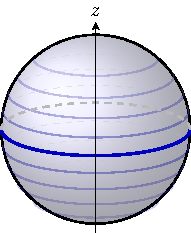
\includegraphics[width=.9\textwidth]{convert/integral-ball}            
          \end{center}
        \end{column}
    \end{columns}
\end{frame}

\begin{frame}
    \frametitle<presentation>{Das Volumen der Einheitskugel}
    \begin{itemize}
        \item Betrachten wir den Schnitt der Kugel mit der $xz$-Ebene, so sehen wir, dass $r(z)=\sqrt{1-z^2}$
        \item Integral über die Kreisflächen
        \begin{gather*}
            V = \int_{-1}^1 A\bigl(r(z)\bigr)\,dz
            = \int_{-1}^1 A\Bigl(\sqrt{1-z^2}\Bigr)\,dz
            = \pi \int_{-1}^1 \bigl(1-z^2\bigr)\,dz
        \end{gather*}
        \item Einsetzen der Stammfunktionen ergibt
        \begin{gather*}
            \int_{-1}^1 \bigl(1-z^2\bigr)\,dz
            = \left[ z-\frac{z^3}3\right]_{-1}^1
            = \left(1-\frac13\right) - \left(-1 - \frac13\right)
            = \frac43
        \end{gather*}
        \item Wir erhalten das Volumen
        \begin{gather*}
            V = \frac43\pi
        \end{gather*}
    \end{itemize}
\end{frame}

\begin{Aufgabe}
    Berechnen Sie das Volumen $V(r)$ einer Kugel vom Radius $r$.
\end{Aufgabe}

\begin{frame}{Berechnung von Volumina}
    Aus der Berechnung des Kugelvolumens können wir ein allgemeines Prinzip der Berechnung von Volumina ableiten:

    \begin{enumerate}
        \item Wir wählen eine \glqq{}Achse\grqq{} im Raum
        \item Wir bestimmen für jeden Punkt der Achse die Fläche des Schnitts in der Ebene senkrecht zu dieser Achse
        \begin{itemize}
            \item Eventuell ist hier auch Integration nötig
        \end{itemize}
        \item Wir integrieren diese Flächen entlang der Achse
    \end{enumerate}
\end{frame}

\begin{Aufgabe}
    Berechnen Sie das Volumen des Rotationskörpers (schlagen Sie den Begriff ggf.\ nach), der auf der $z$-Achse zwischen $-\pi/2$ und $\pi/2$ liegt und dessen Radius
    \begin{gather*}
        r(z) = \cos z
    \end{gather*}
    ist.
\end{Aufgabe}

\begin{Aufgabe}
    \begin{minipage}[b]{.64\textwidth}
      Ein geschraubter Zylinder habe folgende Maße:
      \begin{gather*}
          z\in[0,2\pi]
      \end{gather*}
    und auf Höhe $z$ sei sein Querschnitt ein Quadrat, dessen Eckpunkte die Koordinaten
      \begin{gather*}
          \begin{pmatrix}
          \cos z\\\sin z
          \end{pmatrix},\;
          \begin{pmatrix}
          -\sin z\\\cos z
          \end{pmatrix},\;
          \begin{pmatrix}
          -\cos z\\ -\sin z
          \end{pmatrix},\;
          \begin{pmatrix}
          \sin z\\-\cos z
          \end{pmatrix}
      \end{gather*}
      haben. Berechnen Sie sein Volumen!
    \end{minipage}
    \begin{minipage}[b]{.35\textwidth}
    \begin{center}
    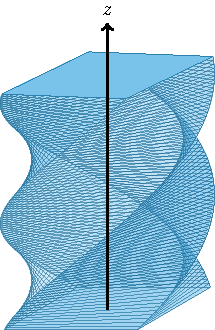
\includegraphics[width=.9\textwidth]{convert/integral-helix}
    \end{center}
    \end{minipage}
\end{Aufgabe}

\mode<all>

%\mode*

\section{Kurven: Pfade und Wege}

%%%%%%%%%%%%%%%%%%%%%%%%%%%%%%%%%%%%%%%%%%%%%%%%%%%%%%%%%%%%
\begin{frame}
    \begin{Denkpause}
        Auf einer Wanderung bewegen Sie sich durch eine Landschaft. Was für ein mathematisches Objekt ist geeignet, diese Bewegung zu beschreiben.
    \end{Denkpause}
\end{frame}

\begin{frame}{Definition: Weg}
    Ein Weg ist eine Abbildung von einem Zeitintervall $I$ in einen Vektorraum, zum Beispiel $\R^n$.
\end{frame}
%%%%%%%%%%%%%%%%%%%%%%%%%%%%%%%%%%%%%%%%%%%%%%%%%%%%%%%%%%%%
\begin{frame}{Analytische Eigenschaften von Pfaden}
    \begin{itemize}
        \item Stetigkeit, Differenzierbarkeit und Integrale von Pfaden sind komponentenweise definiert.
        \item Ableitungen
        \begin{gather*}
            \vf'(t) = \tfrac{d}{dt}
            \begin{pmatrix}
                \tfrac{d}{dt} f_1(t)\\
                \vdots\\
                \tfrac{d}{dt} f_n(t)
            \end{pmatrix}
            = \begin{pmatrix}
                f_1'(t)\\\vdots\\f_n'(t)
            \end{pmatrix}
        \end{gather*}
        \item Integrale
        \begin{gather*}
            \int \vf(t)\,dt = \vF(t),
        \qquad F_i(t) = \int f_i(t)\,dt,\quad i=1,\dots,n
        \end{gather*}
    \end{itemize}
\end{frame}

%%%%%%%%%%%%%%%%%%%%%%%%%%%%%%%%%%%%%%%%%%%%%%%%%%%%%%%%%%%%
\begin{frame}{Beispiele in zwei Dimensionen}
    \begin{columns}
        \begin{column}[t]{.5\textwidth}
        \begin{block}{Geradlinige Bewegung}
            \begin{align*}
                x(t) &= f_1(t) = x_0 + t u\\
                y(t) &= f_2(t) = y_0+tv
            \end{align*}
            oder in Vektorschreibweise
            \begin{gather*}
                \vx(t) = \vx_0+t\vv
            \end{gather*}
            Ableitung
            \begin{gather*}
                \vx'(t) = \vv
            \end{gather*}
        \end{block}         
        \end{column}
        \pause
        \begin{column}[t]{.5\textwidth}
        \begin{block}{Kreisbewegung}
            \begin{align*}
                x(t) &= r \cos t\\
                y(t) &= r \sin t
            \end{align*}
            mit der Ableitung
            \begin{align*}
                x(t) &= -r \sin t\\
                y(t) &= r \cos t
            \end{align*}
        \end{block}         
        \end{column}
    \end{columns}
\end{frame}

%%%%%%%%%%%%%%%%%%%%%%%%%%%%%%%%%%%%%%%%%%%%%%%%%%%%%%%%%%%%
\begin{frame}{Definition Weg}
\mrerror{Warum wird "Weg" nochmal definiert, wenn dies bereits in 2.0.1 geschieht?}    
\end{frame}

\begin{envgknote}{hinzufügen}
   \begin{itemize}
       \item Wege: parametrische und nullstellen-Darstellung
       \item Begriffsklärung
       \item Beispiele Gerade und Kreis
       \item zu einem Weg kann es mehrere Pfade geben, die ihn parametrisieren
       \item Beispiel chemische Reaktion oder Biosystem
       \item Wann ist ein Weg als $y=f(x)$ darstellbar?
       \item Implizite Differentiation
   \end{itemize} 
\end{envgknote}

\mrnote{Folgende passenden Folien sind provisorisch aus der alten Vorlesung entnommen:}

%%%%%%%%%%%%%%%%%%%%%%%%%%%%%%%%%%%%%%%%%%%%%%%%%%%%%
\begin{frame}
    \frametitle{Darstellung eines Weges als Funktion}

    Unter welchen Bedingungen lässt sich ein Weg auch als \grqq klassischer \grqq Graph einer Funktion $y=f(x)$ betrachten?

    \begin{itemize}
        \item Bewegung eines Punktes auf einen festen Kreis
    \begin{columns}
        \begin{column}{0.5\textwidth}
    $$
    \left\{\begin{array}{l}
        x(t) = a\cos(\omega t)\\ y(t) = a\sin(\omega t)
    \end{array}\right.
    $$
\end{column}
\begin{column}{0.5\textwidth}
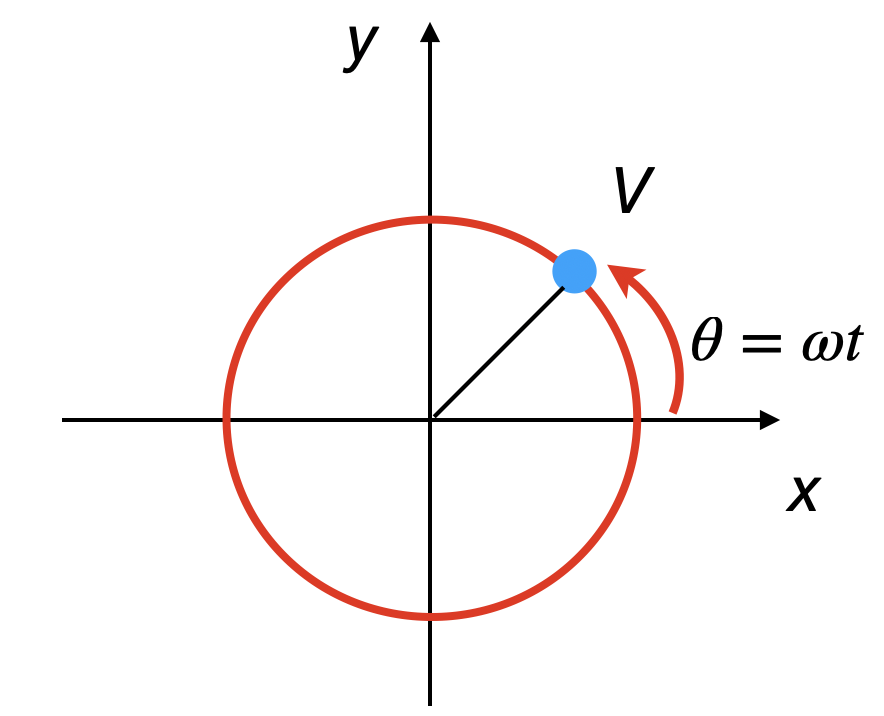
\includegraphics[width=0.5\textwidth]{fig/pk03.png}
\end{column}
\end{columns}
    \item $\sin(\omega t) = \sqrt{1-\cos^2(\omega t)}$ (nur für die obere Kreishälfte!)
    \item Daher:
    \begin{multline}
    y(t) = a\sin(\omega t) \Longrightarrow y(t) = a \sqrt{1-\cos^2(\omega t)} \\ 
    \Longrightarrow y(t) = \sqrt{a^2-a^2\cos^2(\omega t)} \Longrightarrow y(t) = \sqrt{a^2-x(t)^2} 
    \end{multline}
    \item Also: $y = f(x) = \sqrt{a^2-x^2}$ (obere Kreishälfte)
\end{itemize}


\end{frame}

\mode<all>

%\mode*
\section{Mehrdimensionale Funktionen}

\begin{frame}{Arten mehrdimensionaler Funktionen}
\begin{enumerate}
    \item Funktionen einer Variablen, die in $\R^n$ abbilden (Wege):
    \begin{gather*}
        \vf\colon \R\to \R^n,\qquad t\mapsto \vf(t)
    \end{gather*}
    \item Funktionen mehrerer Variablen, die nach $\R$ abbilden:
    \begin{gather*}
        f\colon \R^m\to \R,\qquad \vx \mapsto f(\vx)
    \end{gather*}
    \item Funktionen mehrerer Variablen, die in $\R^n$ abbilden:
    \begin{gather*}
        \vf\colon \R^m \to \R^n,\qquad \vx \mapsto \vf(\vx)
    \end{gather*}
\end{enumerate}
Notation: wir schreiben Vektorgrößen als $\vx,\vy,\vf$ zur Unterscheidung von Zahlen $t,x,f$.
\end{frame}

\subsection{Darstellung}

\begin{frame}{Höhenlinien}
  \begin{center}
    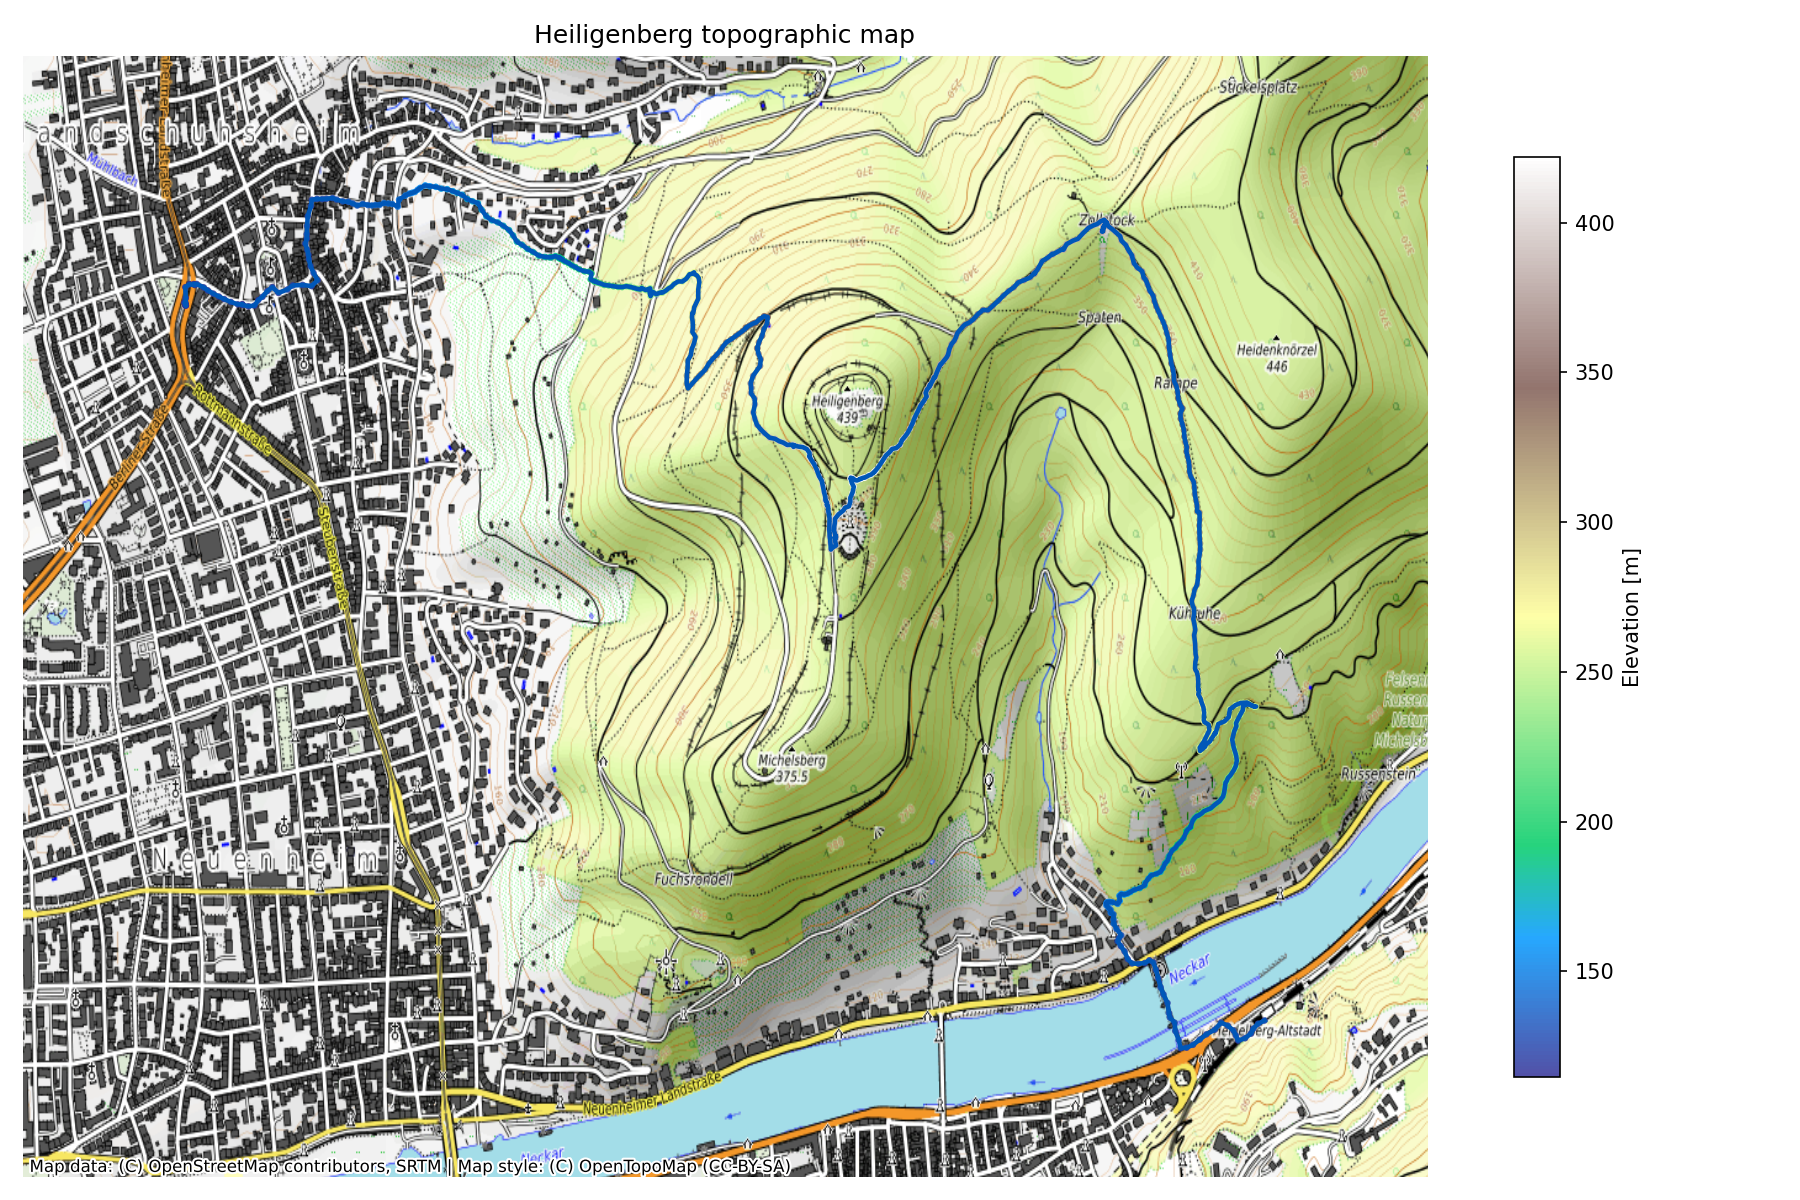
\includegraphics[width=.9\textwidth]{pic/topography_map}
  \end{center}
\end{frame}

\begin{frame}{Oberflächendiagramm (surface plot)}
  \begin{center}
    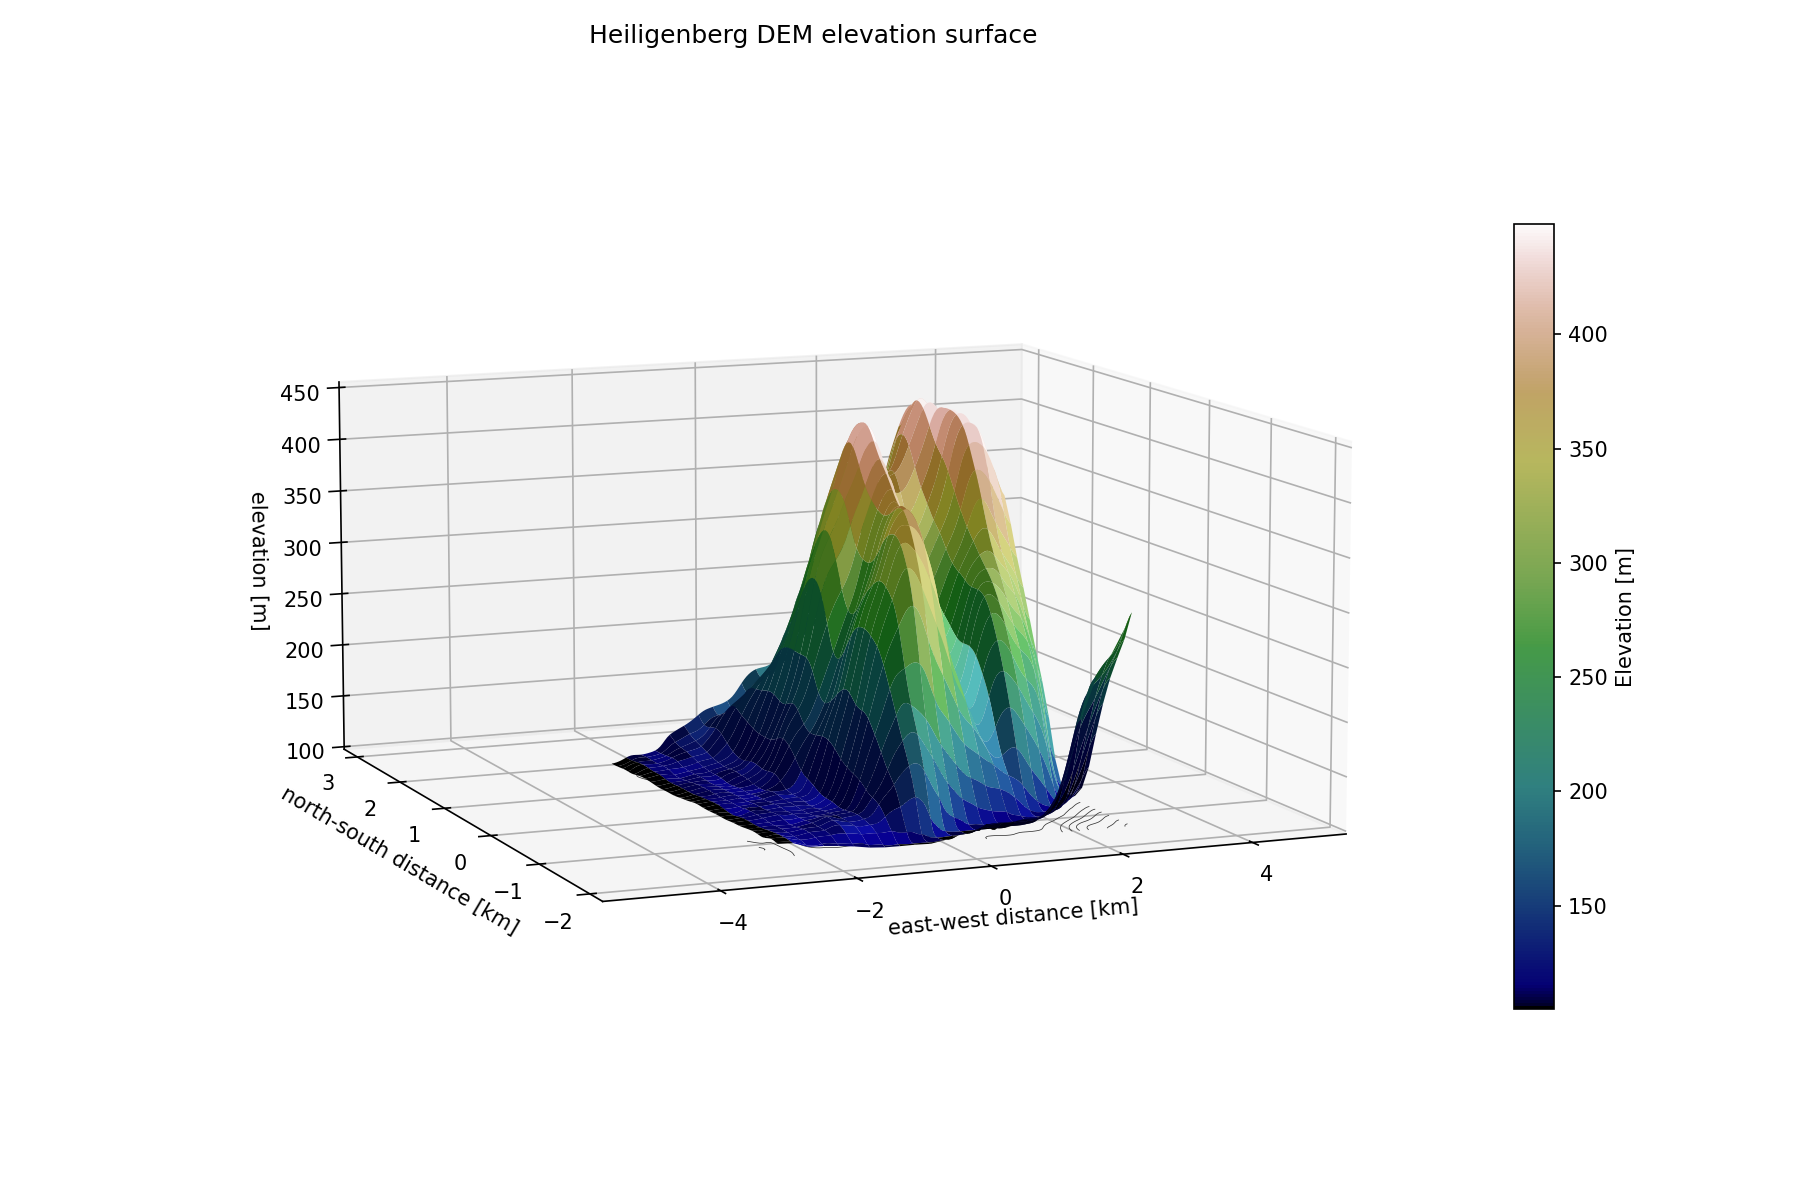
\includegraphics[width=.9\textwidth]{pic/topography_surface}
  \end{center}
\end{frame}

% \begin{frame}{Isoflächen}
%     \begin{columns}
%         \begin{column}{.5\textwidth}
%             \begin{gather*}
%                 f:\R^3\to \R
%             \end{gather*}
%         \end{column}
%         \begin{column}{.5\textwidth}
%             \begin{center}
% %                \includegraphics[width=\textwidth]{fig/Benzene_density_isosurface.png}
%                 Benzol, Elektronendichte
%             \end{center}
%             \tiny Xavier Andrade, CC BY-SA 3.0, via Wikimedia Commons
%         \end{column}
%     \end{columns}
% \end{frame}

\subsection{Partielle Ableitungen}
\mrnote{Provisorisch sind die Folien aus Carl Herrmanns Teil zu partiellen Ableitungen eingefügt}

%%%%%%%%%%%%%%%%%%%%%%%%%%%%%%%%%%%%%%%%%%%%%%%%%%%%%
\begin{frame}
    \frametitle{Partielle Ableitungen}

\begin{itemize}
    \item Eine Raumdimension
    \begin{itemize}
        \item Die Ableitung $\frac{df(t)}{dt}$ beschreibt die {\bf Änderung} von $f(t)$ bei infinitesimalen Veränderungen von $t$
    \end{itemize}
    \item {\bf Partielle Ableitung}: Änderung der Funktion $f(x_1,\ldots,x_n)$ bei infinitesimalen Veränderungen {\bf einer} Variablen, wobei die anderen {\bf konstant} bleiben!
\end{itemize}
    \begin{gather*}
        \frac{f(x_1,\ldots,x_k+h, \ldots, x_n) - f(x_1,\ldots, x_n)}{h} \xrightarrow{h \to 0} \frac{\partial f(x_1,\ldots,x_n)}{\partial x_k}  
    \end{gather*}
\end{frame}
 
%%%%%%%%%%%%%%%%%%%%%%%%%%%%%%%%%%%%%%%%%%%%%%%%%%%%%
\begin{frame}
    \frametitle{Notation}

    \begin{itemize}

        \item Schreibweisen:
        $$
        \frac{\partial f}{\partial x_k}=\partial_{x_k} f =f_{x_k}=f_{k}
        $$
        \item Beispiele:
        \begin{xalignat*}3
            f(x,y) &= x^2+y^2 & \partial_x f &= 2x &\partial_y f &= 2y \\
            f(x,y) &= 3x^2y^3 & \partial_x f &= 6xy^3 & \partial_y f &= 9x^2y^2
        \end{xalignat*}
    \end{itemize}
\end{frame}


%%%%%%%%%%%%%%%%%%%%%%%%%%%%%%%%%%%%%%%%%%%%%%%%%%%%
\begin{frame}
    \frametitle{Mehrfache Ableitungen}

    \begin{itemize}
        \item Wie bei Funktionen einer Variablen können wir mehrfache Ableitungen berechnen
        \item Alle Kombinationen von Variablen sind möglich!
        \item z.B.\ bei $f(x_1,\ldots,x_k)$:
        $$
        f_{ij} = \frac{\partial^2 f}{\partial x_i \partial x_j} =  \frac{\partial}{\partial x_i}\left(\frac{\partial f}{\partial x_j}\right)
        $$
    \end{itemize}
\end{frame}

%%%%%%%%%%%%%%%%%%%%%%%%%%%%%%%%%%%%%%%%%%%%%%%%%%%%%
\begin{frame}
    \frametitle<presentation>{Vertauschung von Ableitungen}

    Bei Mehrfachableitungen spielt die Reihenfolge der Ableitungen (bei den Funktionen, die wir betrachten) keine Rolle! (Satz von Schwarz)
\vspace{1em}

    {\bf Beispiel:} $f(x,y,z) = e^{xy^2}\,\sin z$
    \begin{itemize}
        \item $f_x = y^2\,e^{xy^2}\,\sin z$ , $f_y = 2xy\,e^{xy^2}\,\sin z$
        \item bei doppelten Ableitungen gilt: $f_{xy}=f_{yx}$
    \end{itemize}
    \vspace{3cm}

\end{frame}



%%%%%%%%%%%%%%%%%%%%%%%%%%%%%%%%%%%%%%%%%%%%%%%%%%%%%
\begin{frame}
    \frametitle{Partielle Ableitungen und Tangente}

\begin{center}
    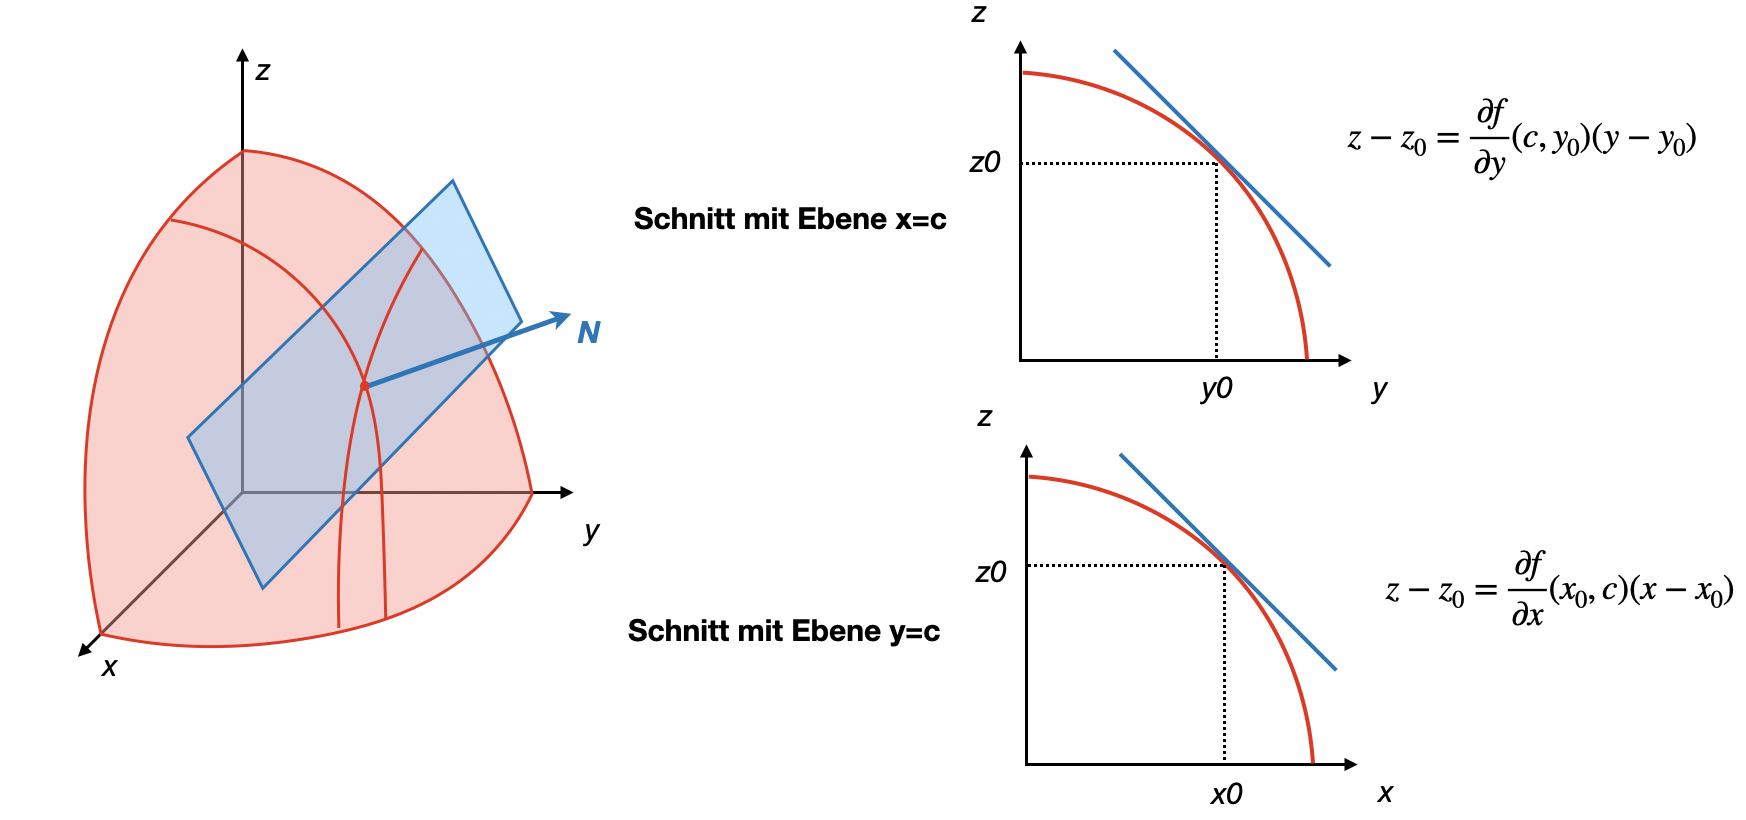
\includegraphics[width=.8\textwidth]{fig/mv10.png}
\end{center}
\begin{itemize}
    \item Gleichung der Tangentialebene am Punkte $(x_0,y_0)$:
    \begin{gather*}
    z-z_0 = \frac{\partial f}{\partial x}(x_0,y_0) (x-x_0) +\frac{\partial f}{\partial y}(x_0,y_0) (y-y_0)         
    \end{gather*}
    \item Normalenvektor zur Ebene:
    $$
    N = (\frac{\partial f}{\partial x}(x_0,y_0), \frac{\partial f}{\partial y}(x_0,y_0),-1)
    $$
\end{itemize}
\end{frame}

%%%%%%%%%%%%%%%%%%%%%%%%%%%%%%%%%%%%%%%%%%%%%%%%%%%%%
\begin{frame}
    \frametitle{Beispiel}

    Wir berechnen die Gleichung der Tangentialebene für die Funktion $z=x^2-y-xe^y$ am Punkt $(x_0,y_0) = (1,0)$:
    \begin{eqnarray*}
    f_x = 2x-e^y &;& f_x(1,0) = 1 \\
    f_y = -1-xe^y &;& f_y(1,0) = -2
    \end{eqnarray*}
    Da $z_0=f(1,0) = 0$ gilt folgende Gleichung:
    $$
    z -z_0 = f_x(1,0)(x-1) + f_y(1,0)(y-0) \iff z = x-1 -2y 
    $$

    Normalenvektor:
    $$
    N = (1,-2,-1)
    $$
\end{frame}

%%%%%%%%%%%%%%%%%%%%%%%%%%%%%%%%%%%%%%%%%%%%%%%%%%%%%
\begin{frame}
    \frametitle{Gradient einer Funktion}

    \begin{itemize}
        \item Wir definieren den {\bf Gradienten} der Funktion $f$:
        $$
    \nabla f = \left(\begin{array}{c} \partial_{x_1}f \\ \vdots \\  \partial_{x_n}f \end{array}\right)
        $$
        \item $\nabla f(p)$ ist ein Vektor in $\mathbb{R}^n$ am Punkt $p$
        \item Beispiel: $f(x,y) = 3x^2y^3$:
        $$
        \nabla f = \left(\begin{array}{c} 6xy^3 \\ 9x^2y^2 \end{array}\right) ~~\rightarrow~~ \nabla f(1,1) = \left(\begin{array}{c} 6 \\ 9 \end{array}\right)
        $$
\end{itemize}
\end{frame}

%%%%%%%%%%%%%%%%%%%%%%%%%%%%%%%%%%%%%%%%%%%%%%%%%%%%%%%%%%%%
%%%%%%%%%%%%%%%%%%%%%%%%%%%%%%%%%%%%%%%%%%%%%%%%%%%%%%%%%%%%
\subsection{Richtungsableitungen}

\begin{frame}
    \frametitle{Veränderungen in beliebige Richtungen}

    \begin{itemize}
        \item Die partiellen Ableitungen $\partial_x f$ unf $\partial_y f$ beschreiben die Veränderungen von $z=f(x,y)$ wenn man sich in $x-$ bzw $y-$Richtung bewegt
        \item Wie verändert sich die Funktion, wenn man sich in eine beliebige Richtung bewegt?
        \item Richtung gegeben durch Vektor $\vu$
        \item {\bf Richtungsableitung} (in 2 Dimensionen):
        $$
        D_u f = \frac{\partial f}{\partial x}\cdot u_1 + \frac{\partial f}{\partial y}\cdot u_2
        $$
    \end{itemize}
    \begin{center}
        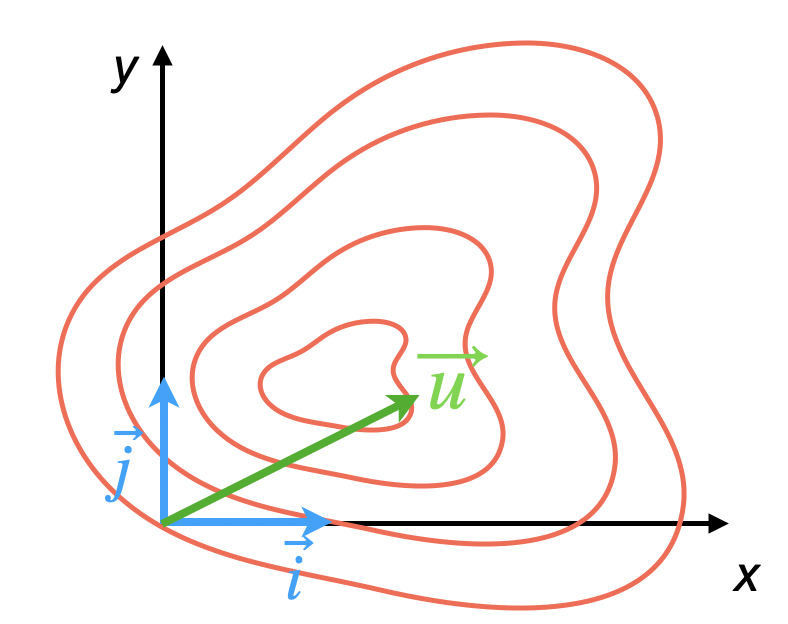
\includegraphics[width=.3\textwidth]{img/mv17.png}
    \end{center}

\end{frame}

%%%%%%%%%%%%%%%%%%%%%%%%%%%%%%%%%%%%%%%%%%%%%%%%%%%%%
\begin{frame}
    \frametitle{Richtungsableitung}

    \begin{itemize}
        \item Schreibweise mit Gradient (Skalarprodukt!):
        $$
        D_u f = \nabla f \cdot \vu
        $$
        \item $D_u f(p)$ gibt an, wie stark die Steigung in $\vu$-Richtung am Punkt $p$ ist
        \item $D_u f(p)>0$ bzw. $D_u f(p)< 0$: es geht nach oben bzw.\ nach unten!
          \pause
        \item Die Richtungsableitung hängt von der Länge des Richtungsvektors ab
          \begin{itemize}
          \item Manche Autoren fordern $\left|\vu\right| = 1$
          \item Wir normieren bei Bedarf
          \end{itemize}
    \end{itemize}
\end{frame}

%%%%%%%%%%%%%%%%%%%%%%%%%%%%%%%%%%%%%%%%%%%%%%%%%%%%%
\begin{frame}
    \frametitle{Richtung konstanter Werte}

    \begin{center}
        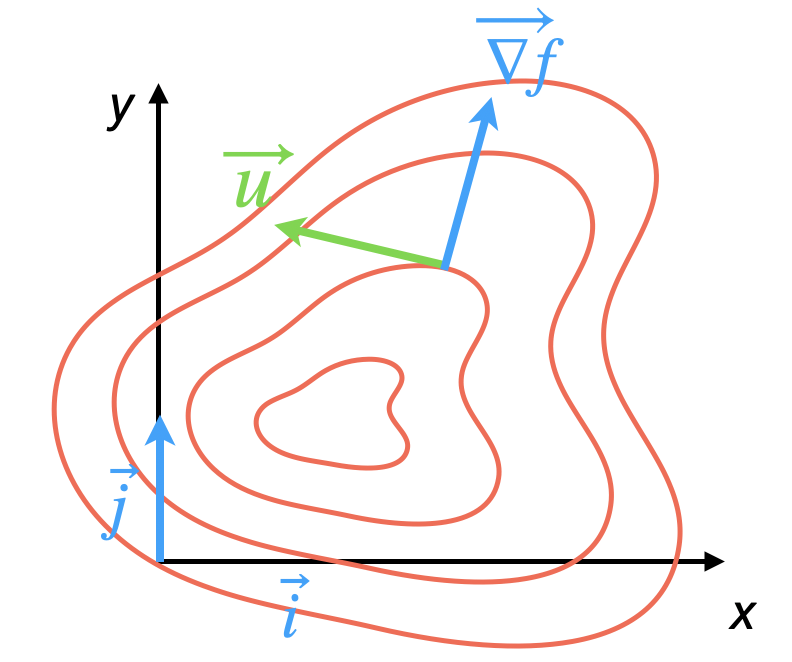
\includegraphics[width=.3\textwidth]{img/mv18.png}
    \end{center}

    \begin{itemize}
        \item In welche Richtung verändert sich die Funktion {\bf nicht}?
        $$
        D_u f = 0 ~\iff~ \nabla f \cdot \vu =0 ~\iff ~ \nabla f \perp \vu
        $$
        \item $\vu$ ist ein {\bf Tangentialvektor} zu den Höhenlinien!
    \end{itemize}
\end{frame}
%%%%%%%%%%%%%%%%%%%%%%%%%%%%%%%%%%%%%%%%%%%%%%%%%%%%%
\begin{frame}
    \frametitle{Abstiegs- und Aufstiegsrichtungen}

    \begin{center}
        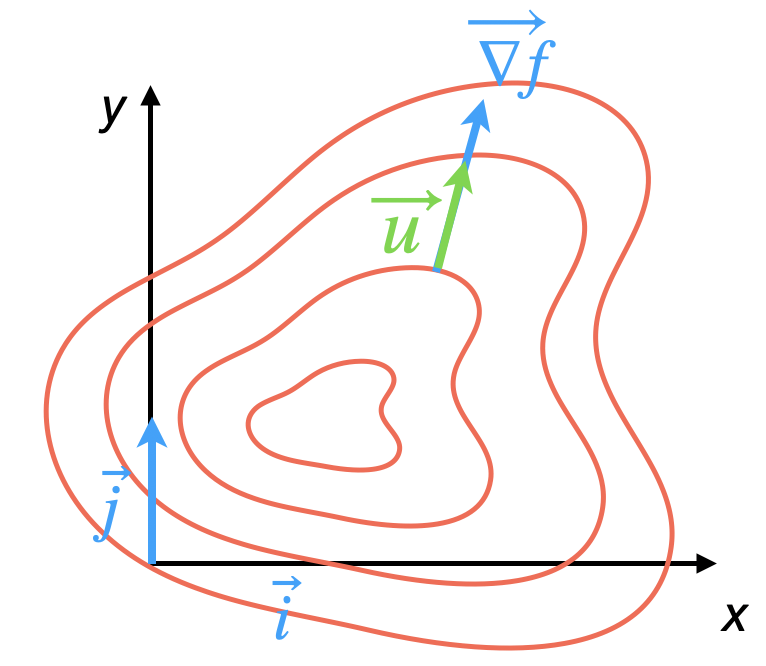
\includegraphics[width=.3\textwidth]{img/mv19.png}
    \end{center}

    \begin{itemize}
        \item In welche Richtung ist die Veränderung {\bf am größten}?
        $$
        \max_{\vu} D_u f ~\iff ~ \vu \parallel\nabla f
        $$
        \item Wenn $\vu$ Einheitsvektor: $\vu=\frac{\nabla f}{|\nabla f|}$; daher
        $
        D_u f = \nabla f \cdot \frac{\nabla f}{|\nabla f|} = |\nabla f|
        $
        \item Der Gradient gibt an jedem Punkt die Richtung der {\bf größten Veränderung} (orthogonal zu den  Höhenlinien)
    \end{itemize}
\end{frame}

%%%%%%%%%%%%%%%%%%%%%%%%%%%%%%%%%%%%%%%%%%%%%%%%%%%%%
\begin{frame}
    \frametitle{Beispiel}

    \begin{itemize}
        \item $f(x,y) = \frac{1}{2}(14-x^2-y^2)$
        \item Gradient:
          \begin{gather*}
            \nabla f =
            \begin{pmatrix}
              -x\\-y
            \end{pmatrix}
          \end{gather*}
        \item Am Punkt $(x_0,y_0) = (1,2)$: $z_0 = \nicefrac92$
        $$
        \nabla f (x_0,y_0) = \left(\begin{array}{c}-1 \\ -2\end{array}\right)
        $$

        \end{itemize}
    \end{frame}

   %%%%%%%%%%%%%%%%%%%%%%%%%%%%%%%%%%%%%%%%%%%%%%%%%%%%%
   \begin{frame}
    \frametitle<presentation>{Beispiel}

    \begin{itemize}
        \item Größte Steigung am Punkt $(x_0,y_0)$:
        $$
            |\nabla f (x_0,y_0)| = \sqrt{\left(-1\right)^2+\left(-2\right)^2} = \sqrt{5}
        $$
        \item Richtung der Höhenlinien: entlang der Höhenlinien ist die Steigung Null; daher erfüllt der Tangentialvektor zu den Höhenlinien die Bedingung:
        $$
        \nabla f (x_0,y_0)\cdot \vu = 0 ~\iff~ \vu ~~\parallel~~ \left(\begin{array}{c}2 \\ -1\end{array}\right)
        $$
        \item Einheitsvektor:  $\vec{e}_u = \frac{\vu}{|\vu|} ~\Rightarrow~ \vec{e}_u= \frac{1}{\sqrt{5}}\left(\begin{array}{c}2 \\ -1\end{array}\right) $
    \end{itemize}
\end{frame}

        \item Die Fläche eines Dreiecks ist gegeben durch $A(a,b,\theta) = \frac{1}{2}ab\sin\theta$; bestimmen Sie das totale Differential  !
        \item Das Volumen eines Zylinders ist $V=\pi r^2 h$; verändert sich das Volumen mehr, wenn $r$ von $1.0$ auf $1.1$ oder $h$ von $1.0$ auf $1.1$ erhöht wird?
    \end{enumerate}
\end{frame}

%%%%%%%%%%%%%%%%%%%%%%%%%%%%%%%%%%%%%%%%%%%%%%%%%%%%%%%%%%%%
\begin{frame}{Ableitung entlang eines Weges}
  \begin{itemize}
  \item Wir bewegen uns entlang eines Weges $\vx(t)$ im Raum
  \item Im Raum ist eine differenzierbare Funktion $f(\vx)$ definiert
  \item Wie ändert sich der Wert dieser Funktion abhängig von $t$?
  \item Kettenregel:
    \begin{gather*}
      \frac{d}{dt} f(\vx(t)) = \nabla f(\vx(t)) \cdot \vx'(t)
    \end{gather*}
  \end{itemize}
\end{frame}

%%%%%%%%%%%%%%%%%%%%%%%%%%%%%%%%%%%%%%%%%%%%%%%%%%%%%%%%%%%%
\begin{frame}{Beispiel}
  \begin{gather*}
    f(\vx) = \tfrac12(x^2+y^2),\qquad
    \nabla f =
    \begin{pmatrix}
      x\\y
    \end{pmatrix}
  \end{gather*}
  \begin{itemize}
  \item Kreislinie:
    \begin{gather*}
      \vx(t) =
      \begin{pmatrix}
        \cos t\\\sin t
      \end{pmatrix},
      \qquad
      \vx'(t) =
      \begin{pmatrix}
        -\sin t\\\cos t
      \end{pmatrix},
      \qquad
      \nabla f(\vx)\cdot \vx'(t) = 0
    \end{gather*}
    \pause
  \item Gerade durch null:
    \begin{gather*}
      \vx = \sqrt2
      \begin{pmatrix}
        t\\t
      \end{pmatrix},\qquad
      \vx'(t) =
      \begin{pmatrix}
        1\\1
      \end{pmatrix},
      \qquad
      \nabla f(\vx)\cdot \vx'(t) = t
    \end{gather*}
  \end{itemize}
\end{frame}

\begin{envgknote}{Neue Struktur}
    \begin{itemize}
    \item Höhenlinien- und Schnittliniendiagramme (Vorlesung 3.1)
    \item Isoflächen, Orbitale?
    \item Partielle Ableitungen, Gradient, Richtungsableitungen
    \item Extremwertaufgaben über Variationsprinzip (Vorlesung 3.4)
    \item Gradient Descent (Vorlesung 3.6)
    \item Optimierung mittels Lagrange-Multiplikatoren (Vorlesung 3.7)
    \end{itemize}
\end{envgknote}

\begin{envmrerror}{Ergänzungen aus der aktuellen Vorlesung}
\begin{itemize}
    \item Schnittliniendiagramme (Vorlesung 3.1)
    \item Fehlerfortpflanzung additiver und multiplikativer Fehler (Vorlesung 3.3). Hier könnte überlegt werden, ob ausgehend von der bestehenden Vorlesung ein Übergang zum Kapitel 4 \textit{Auswirkung von Eingabe- und Rechenfehlern} gemacht werden könnte.
    \item Extremwertaufgaben, Hesse-Matrix, Definitheit von Matrizen (Vorlesung 3.4)
    \item Optimierung mittels Lagrange-Multiplikatoren (Vorlesung 3.7)
    \item Richtungsableitungen (Vorlesung 3.5)    
    \item Gradient Descent (Vorlesung 3.6)
\end{itemize}
\end{envmrerror}

\begin{envmrnote}{Mögliche Klausuraufgaben}
\begin{itemize}
    \item Zuordnung von Höhenlinien/Schnittlinien-Diagrammen zu Plots von Funktionen
    \item Analyse und Interpretation von Funktionen anhand von gegebenen Höhenlinien/Schnittliniendiagrammen oder selbstständig geeignete Höhen/Schnittebenen zur Funktionsanalyse finden und diese Auswahl begründen
\end{itemize}
\end{envmrnote}

  

\mode<all>

%\mode*
\section{Optimierung}

%%%%%%%%%%%%%%%%%%%%%%%%%%%%%%%%%%%%%%%%%%%%%%%%%%%%%%%%%%%% 
%%%%%%%%%%%%%%%%%%%%%%%%%%%%%%%%%%%%%%%%%%%%%%%%%%%%%%%%%%%%
\subsection{Lagrange-Multiplikatoren}

\begin{frame}{Minimierung mit Nebenbedingungen}
  Aufgabe dieses Abschnitts: finde $\vx^* \in \R^n$, so dass
  \begin{gather*}
    f(\vx)
  \end{gather*}
  minimiert wird, unter der Nebenbedingung, dass
  \begin{gather*}
    g(\vx^*)=0 
  \end{gather*}
  gilt. Analog kann natürlich auch maximiert werden.
\end{frame}

%%%%%%%%%%%%%%%%%%%%%%%%%%%%%%%%%%%%%%%%%%%%%%%%%%%%%
\begin{frame}
  \frametitle{Einfaches Beispiel}  
  \begin{itemize}
  \item Wir suchen den/die Punkt(e) auf der Hyperbel $xy=3$, der/die am nächsten am Ursprung liegt
  \end{itemize}
  \begin{center}
    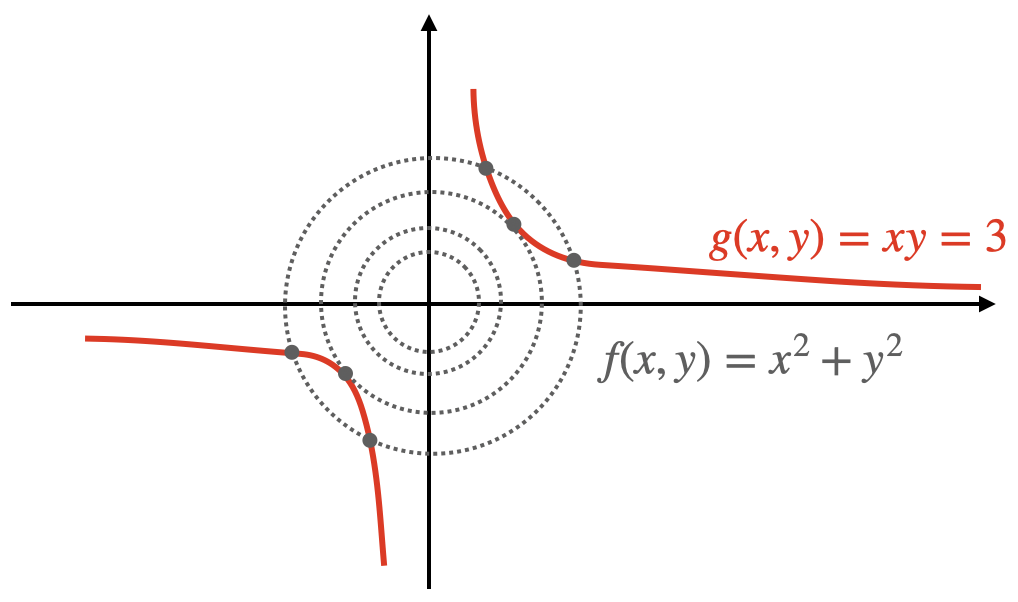
\includegraphics[width=0.7\textwidth]{img/mv22.png}
  \end{center}
  
  \begin{itemize}
  \item Geometrische Lösung: Berührungspunkt vom kleinstmöglichen Kreis um den Ursprung und der Hyperbel
  \end{itemize}
\end{frame}

\begin{frame}
  \frametitle<presentation>{Einfaches Beispiel: mathematische Formulierung}
  Finde das $\vx^*=(x,y)$, so dass
  \begin{gather*}
    f(\vx) = x^2+y^2
  \end{gather*}
  minimal ist, und die Nebenbedingung
  \begin{gather*}
    g(\vx^*) = xy -3 = 0
  \end{gather*}
  gilt.
  \begin{itemize}
  \item Die Wurzelfunktion ist monoton, wir können also das Quadrat minimieren.
  \end{itemize}
\end{frame}

\begin{frame}
  \frametitle<presentation>{Einfaches Beispiel: Eigenschaften}
  \begin{center}
    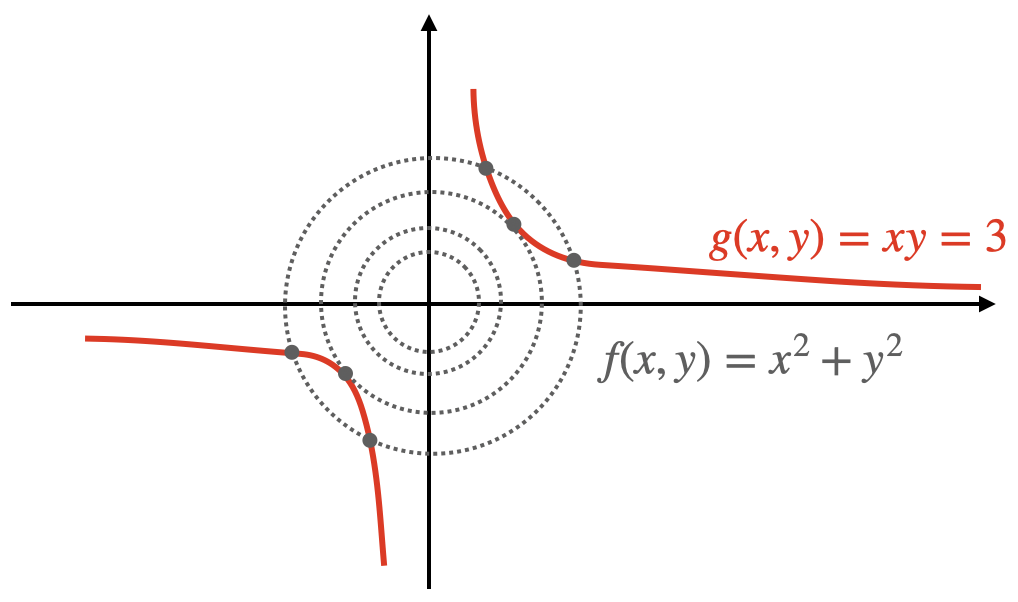
\includegraphics[width=0.6\textwidth]{img/mv22.png}
  \end{center}

  \begin{itemize}
  \item Die Eigenschaft $\nabla f=0$ gilt nur im Ursprung, ist also hier nicht anwendbar
  \item Parametrisiere die Kurve $xy-3=0$ mit $\vx(t)$,
    so dass $\vx^*=\vx(0)$
  \item Dort gilt die eindimensionale Minimalbedingung
    \begin{gather*}
      d_t f(\vx(0)) = \nabla f(\vx(0))\cdot \vx'(0) = 0
    \end{gather*}
  \end{itemize}
\end{frame}

%%%%%%%%%%%%%%%%%%%%%%%%%%%%%%%%%%%%%%%%%%%%%%%%%%%%%%%%%%%%
\begin{frame}
  \frametitle<presentation>{Einfaches Beispiel: Lagrange-Multiplikator}
  \begin{center}
    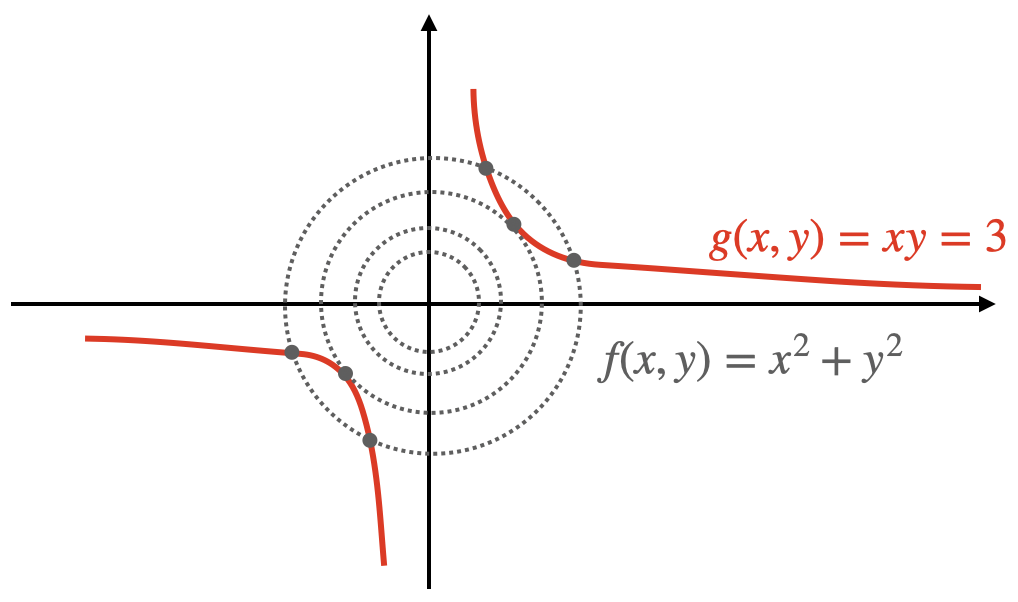
\includegraphics[width=0.6\textwidth]{img/mv22.png}
  \end{center}
  
  \begin{itemize}
  \item Es ist also der Tangentialvektor von $\vx(t)$ orthogonal zu $\nabla f$.
  \item Der Tangentialvektor einer Kurve ist auch orthogonal zum Gradienten (s. Kap. 2)
  \item Es ist also $\nabla f(\vx^*)$ parallel zu $\nabla g(\vx^*)$ und es gibt $\lambda$ mit
    \begin{gather*}
      \nabla f(\vx^*) = \lambda \nabla g(\vx^*)
    \end{gather*}
  \item $\lambda$ heißt \textbf{Lagrange-Multiplikator}
  \end{itemize}  
\end{frame}

\begin{frame}
  \frametitle<presentation>{Einfaches Beispiel: Lagrange-System}
  \begin{itemize}
  \item Wir suchen nun die Lösung $(\vx^*,\lambda)$ des Systems
    \begin{gather*}
      \begin{aligned}
        \nabla f(\vx^*) - \lambda \nabla g(\vx^*) &= 0\\
        g(\vx^*) &=0
      \end{aligned}
      \quad\Leftrightarrow\quad
      \begin{aligned}
      \begin{pmatrix}
        2 & -\lambda\\-\lambda & 2
      \end{pmatrix}
        \begin{pmatrix}
          x^*\\y^*
        \end{pmatrix}
        &= 0\\
          x^*y^*-3 &= 0
      \end{aligned}
    \end{gather*}
  \item Für beliebiges $\lambda$ löst $\vx^*=0$ das LGS, aber nicht die Nebenbedingung
    \only<3->{
    \item Die Matrix muss singulär werden, also
      \begin{itemize}
      \item $\lambda=2$: $x^*=y^*$
      \item $\lambda=-2$: $x^*=-y^*$
      \end{itemize}
    \item Im ersten Fall löst $x^*=y^*=\pm\sqrt{3}$ die Aufgabe.
    \item Im zweiten Fall gibt es keine Lösung, da $xy=3>0$ gelten soll
    }
  \end{itemize}
  \only<2>{
    \begin{Denkpause}
      Wie muss $\lambda$ gewählt werden, damit es weitere Lösungen des LGS gibt?
    \end{Denkpause}
  }
\end{frame}

\begin{frame}{Lagrange-Formalismus}
  \begin{itemize}
  \item Jede Lösung der beschränkten Minimierungsaufgabe ist notwendig
    ein stationärer Punkt der \textbf{Lagrange-Funktion}
    \begin{gather*}
      L(\vx,\lambda) \equiv f(\vx) - \lambda g(\vx)
    \end{gather*}
  \item Die Kandidaten erfüllen damit das Gleichungssystem
    \begin{gather*}
      \nabla L(\vx,\lambda) = 0
      \quad\Leftrightarrow\quad
      \begin{aligned}
        \nabla f(\vx) - \lambda \nabla g(\vx) &= 0\\
        -g(\vx) &=0
      \end{aligned}
    \end{gather*}
  \end{itemize}
  \pause
  \begin{Denkpause}
    Was fehlt?
  \end{Denkpause}
\end{frame}

\begin{frame}{Hinreichende Bedingung}
  \begin{itemize}
  \item Um festzustellen, ob es sich um ein Minimum, Maximum,
    etc. handelt betrachten wir jetzt die Hesse-Matrix
    \begin{gather*}
       H_{L}=\nabla^2_{\vx} L(\vx^*,\lambda) = \nabla^2f(\vx^*) - \lambda \nabla^2 g(\vx^*)
    \end{gather*}
  \item Da nur Punkte mit $g(\vx)=0$ zugelassen sind, sind nur
    Variationen in Richtungen $\vv\perp\nabla g(\vx^*)$ relevant
  \item Ein lokales Minimum genau dann, wenn
    \begin{gather*}
      \nabla L = 0 \quad \wedge \quad
      \vv^TH_{L}\vv \ge 0 \;\forall \vv\perp\nabla g
    \end{gather*}
  \item Ein lokales Maximum genau dann, wenn
    \begin{gather*}
      \nabla L = 0 \quad \wedge \quad
      \vv^TH_{L}\vv \le 0 \;\forall \vv\perp\nabla g
    \end{gather*}
  \end{itemize}
\end{frame}

%%%%%%%%%%%%%%%%%%%%%%%%%%%%%%%%%%%%%%%%%%%%%%%%%%%%%%%%%%%%
\begin{frame}{Beispiel: Oberflächenminimierung}
  \begin{itemize}
  \item Ein stabförmiges Bakterium möchte seine Oberfläche minimieren
  \item Es sei der Einfachheit halber zylinderförmig angenommen
    \begin{itemize}
    \item $h$ Höhe
    \item $r$ Radius
    \end{itemize}
  \item Sein Volumen ist fest: $V = \pi r^2h = V_0$
  \item Die Oberfläche ist $A=2\pi r^2+2\pi r h$
    \begin{itemize}
    \item 2 Deckel je $\pi r^2$
    \item Mantel $2\pi r h$
    \end{itemize}
  \item Die Lagrange-Funktion lautet
    \begin{gather*}
      L(r,h,\lambda) = 2\pi r^2+2\pi r h - \lambda(\pi r^2h - V_0)
    \end{gather*}
  \end{itemize}
\end{frame}

%%%%%%%%%%%%%%%%%%%%%%%%%%%%%%%%%%%%%%%%%%%%%%%%%%%%%%%%%%%%
\begin{frame}
  \frametitle<presentation>{Oberflächenminimierung: kritische Punkte}
  \begin{itemize}
  \item Zunächst:
    \begin{align*}
      0=\partial_r L &= 4\pi r + 2\pi h - 2\lambda \pi rh\\
      0=\partial_h L &= 2\pi r - \lambda \pi r^2
    \end{align*}
  \item Die zweite Gleichung impliziert sofort $\lambda = 2/r$
    \pause
  \item Einsetzen in die erste:
    \begin{gather*}
      0=4\pi r+ 2\pi h - 4 \pi h
      \qquad\Rightarrow\qquad h=2r
    \end{gather*}
  \item Aus der Nebenbedingung bekommen wir
    \begin{gather*}
      V = \pi r^2 h = 2\pi r^3 = V_0
      \quad\Rightarrow\quad r = \sqrt[3]{\frac{V_0}{2\pi}}
    \end{gather*}
  \end{itemize}
\end{frame}

%%%%%%%%%%%%%%%%%%%%%%%%%%%%%%%%%%%%%%%%%%%%%%%%%%%%%%%%%%%%
\begin{frame}
  \frametitle<presentation>{Oberflächenminimierung: Hesse-Matrix}
  \begin{itemize}
  \item Die Hesse-Matrix lautet
    \begin{gather*}
      H_L =
      \begin{pmatrix}
        \partial_{rr} L & \partial_{rh} L\\
        \partial_{hr} L & \partial_{hh} L
      \end{pmatrix}
      = 2\pi
      \begin{pmatrix}
        2-\lambda h & 1-\lambda r\\
        1-\lambda r & 0
      \end{pmatrix}
    \end{gather*}
  \item Einsetzen von $\lambda=2/r$ und $h=2r$ ergibt
    \begin{gather*}
      H_L =
      \begin{pmatrix}
        -4\pi & -2\pi\\
        -2\pi & 0
      \end{pmatrix}
    \end{gather*}
  \item Als nächstes benötigen wir $\nabla g$ \visible<2->{{\color{blue}für $h=2r$}}.
    \begin{gather*}
      \partial_r g = 2\pi r h \visible<2->{{\color{blue}=4\pi r^2}}
      \quad \partial_h g = \pi r^2
      \visible<2->{{\color{blue}\qquad\nabla g = \pi r^2
          \begin{pmatrix}
            4\\1
          \end{pmatrix}
        }}
    \end{gather*}
  \item<2-> Damit erfüllen Vektoren $\vv\perp\nabla g$ die Gleichung $v_2 = -4v_1$
  \end{itemize}
\end{frame}

%%%%%%%%%%%%%%%%%%%%%%%%%%%%%%%%%%%%%%%%%%%%%%%%%%%%%%%%%%%%
\begin{frame}
  \frametitle<presentation>{Oberflächenminimierung: Definitheit}
  \begin{gather*}
    H_L =
    \begin{pmatrix}
      -4\pi & -2\pi\\
      -2\pi & 0
    \end{pmatrix}
  \end{gather*}
  \begin{itemize}
  \item Es genügt, den Vektor $\vv=(1,-4)$ einzusetzen. (Warum?)
    \begin{gather*}
      \vv^T H_L\vv = (1,-4)
      \begin{pmatrix}
        -4\pi + 8\pi\\-2\pi
      \end{pmatrix}
      = 12\pi > 0
    \end{gather*}
  \item Es handelt sich also um ein Minimum
  \end{itemize}
\end{frame}

%%%%%%%%%%%%%%%%%%%%%%%%%%%%%%%%%%%%%%%%%%%%%%%%%%%%%%%%%%%%
\begin{frame}
  \frametitle<presentation>{Oberflächenminimierung: Bemerkung}
  \begin{itemize}
  \item Berechnen wir $\vv^TH_L\vv$ mit $\vv$ parallel zu $\nabla g$, erhalten wir
    \begin{gather*}
      (4,1)
      \begin{pmatrix}
        -4\pi & -2\pi\\
        -2\pi & 0
      \end{pmatrix}
      \begin{pmatrix}
        4\\1
      \end{pmatrix}
      = (4,1)
      \begin{pmatrix}
        -16\pi -2\pi\\-8\pi
      \end{pmatrix}
      = -80 \pi < 0
    \end{gather*}
    \begin{itemize}
    \item Die Matrix $H_L$ ist also auf dem gesamten Raum $\R^2$ indefinit
    \item Relevant ist aber nur $\vv\perp\nabla g$
    \end{itemize}
  \end{itemize}
\end{frame}

%%%%%%%%%%%%%%%%%%%%%%%%%%%%%%%%%%%%%%%%%%%%%%%%%%%%%%%%%%%%
\begin{frame}{Zur Bedeutung des Lagrange-Multiplikators}
  \begin{itemize}
  \item Wir kürzen ab: $L(V,\lambda) = A(V) - \lambda (V-V_0)$
  \item Sei nun $A(V)$ zu jedem $V$ die optimale Fläche, also
    \begin{gather*}
      \nabla L(A(V),\lambda) =
      \begin{pmatrix}
        \partial_V A - \lambda\\
        V-V_0
      \end{pmatrix}
      = 0.
    \end{gather*}
  \item Es gilt also $\lambda = \partial_V A$
  \item Der Lagrange-Multiplikator gibt an, wie sich das Optimum
    verändert, wenn ich die Nebenbedingung variiere
  \end{itemize}
\end{frame}

%%%%%%%%%%%%%%%%%%%%%%%%%%%%%%%%%%%%%%%%%%%%%%%%%%%%%%%%%%%% 
\begin{frame}{Beispiel in drei Dimensionen}
  \begin{itemize}
  \item Finde das Minimum der Funktion
  \begin{gather*}
    f(\vx) \equiv f(x,y,z) = 2x-y+z
  \end{gather*}
  unter der Nebenbedingung
  \begin{gather*}
    g(\vx)\equiv x^2+y^2+z^2-1 = 0
  \end{gather*}
  \item Wir stellen zunächst den Gradienten der Lagrange-Funktion auf
    \begin{gather*}
      \nabla L (\vx,\lambda) =
      \begin{pmatrix}
       \partial_x L (x,y,z,\lambda)\\
       \partial_y L (x,y,z,\lambda)\\
       \partial_z L (x,y,z,\lambda)\\
       \partial_\lambda L (x,y,z,\lambda)
      \end{pmatrix}
      =
      \begin{pmatrix}
        2-2\lambda x\\
        -1-2\lambda y\\
        1-2\lambda z\\
        x^2+y^2+z^2-1
      \end{pmatrix}
      \stackrel!= 0
    \end{gather*}
  \end{itemize}
\end{frame}

\begin{frame}
  \frametitle<presentation>{Beispiel in drei Dimensionen: Rechnung}
  \begin{itemize}
  \item Die drei ersten Gleichungen lassen sich nach $x,y,z$ auflösen
    \begin{gather*}
      x = \frac1\lambda,\qquad y = \frac{-1}{2\lambda},\qquad
      z=\frac1{2\lambda}
    \end{gather*}
  \item Dies setzen wir in die Nebenbedingung ein
    \begin{gather*}
      x^2+y^2+z^2 = \frac1{\lambda^2}+\frac1{4\lambda^2}+\frac1{4\lambda^2}
      = \frac3{2\lambda^2}
      \stackrel!= 1,
    \end{gather*}
    was $\lambda^2=3/2$ ergibt.
  \end{itemize}
  \pause
  \begin{Denkpause}
    Warum erwarten wir zwei Lösungen?
  \end{Denkpause}
\end{frame}

\begin{frame}
  \frametitle<presentation>{Beispiel in drei Dimensionen: Einsetzen}
  \begin{itemize}
  \item Setzen wir nun $\lambda = \pm \sqrt{3/2}$ in die Gleichungen der
    anderen Variablen ein, erhalten wir zwei Punkte
    \begin{gather*}
      \vx_1 = \left(\frac2{\sqrt{6}},\frac{-1}{\sqrt6},\frac{1}{\sqrt6}\right),
      \qquad
      \vx_1 = \left(-\frac2{\sqrt{6}},\frac{1}{\sqrt6},\frac{-1}{\sqrt6}\right)
    \end{gather*}
  \item In diesem Fall ist die Hesse-Matrix $\nabla^2f=0$. Aber:
    \begin{gather*}
      H_L =
      \begin{pmatrix}
        0 & 0 & 0\\
        0 & 0 & 0\\
        0 & 0 & 0
      \end{pmatrix}
      -\lambda
      \begin{pmatrix}
        2 &&\\&2&\\&&2
      \end{pmatrix}
    \end{gather*}
  \item Damit erhalten wir:
    \begin{itemize}
    \item $\lambda = +\sqrt{3/2}$: $\vx_1$ Maximum, $f(\vx_1) = \sqrt6$
    \item $\lambda = -\sqrt{3/2}$: $\vx_2$ Minimum, $f(\vx_2) = -\sqrt6$
    \end{itemize}
  \end{itemize}
\end{frame}

%%%%%%%%%%%%%%%%%%%%%%%%%%%%%%%%%%%%%%%%%%%%%%%%%%%%%%%%%%%%
\begin{frame}{Abschlussfragen}
  \begin{enumerate}
  \item Warum führen wir Langrange-Multiplikatoren ein?
  \item Was wissen wir über die Gradienten der zu minimierenden
    Funktion und der Nebenbedingung im Optimum?
  \item Was ist die Lagrange-Funktion und wie finden wir mit ihr
    kritische Punkte?
  \item Wie ist die Darstellung der verwendeten Hesse-Matrix?
  \item Wie unterscheidet sich die hinreichende Bedingung an Extrema
    vom unbeschränkten Fall?
  \end{enumerate}
\end{frame}

%%%%%%%%%%%%%%%%%%%%%%%%%%%%%%%%%%%%%%%%%%%%%%%%%%%%%%%%%%%%
%%%%%%%%%%%%%%%%%%%%%%%%%%%%%%%%%%%%%%%%%%%%%%%%%%%%%%%%%%%%
\subsection{Steilster Abstieg (gradient descent)}
%%%%%%%%%%%%%%%%%%%%%%%%%%%%%%%%%%%%%%%%%%%%%%%%%%%%%%%%%%%%
\begin{frame}{Wie findet man Minima?}
  Bleiben wir beim Bild der Wanderung
  \only<1>{
    \begin{Denkpause}
      Sie stehen an einem Hang und wollen die Talsohle erreichen. In
      welche Richtung gehen Sie?
    \end{Denkpause}
  }
  \pause
  \begin{itemize}
  \item Nach unten!
  \item Am schnellsten abwärts geht es in Richtung
    \begin{gather*}
      -\nabla f
    \end{gather*}
  \item Das ist die \textbf{Richtung des steilsten Abstiegs}
  \item Daraus leitet sich das \textbf{Verfahren des steilsten
      Abstiegs}, auf Englisch \textbf{gradient descent} ab.
  \item Es wird eingesetzt zur Minimierung, z.B. einer Energie
  \item In der Sprache der Optimierung minimieren wir eine
    \textbf{Kostenfunktion}
  \end{itemize}
\end{frame}

%%%%%%%%%%%%%%%%%%%%%%%%%%%%%%%%%%%%%%%%%%%%%%%%%%%%%%%%%%%%
\begin{frame}{Definition des Verfahrens des steilsten Abstiegs}
  Gradient descent
  \begin{itemize}
  \item Ausgehend von einem \textbf{Startwert} $\vx_0$ generiert das
    Verfahren eine Folge
    \begin{gather*}
      \vx_1,\vx_2,\ldots
    \end{gather*}
    mit dem Ziel, sich dem Minimum anzunähern.
  \item Sei $f(\vx)$ die Kostenfunktion
  \item Nach $n$ Schritten des Verfahrens berechnen wir $\vx_{n+1}$ durch
    \begin{gather*}
      \vx_{n+1} = \vx_{n} - \eta \nabla f(\vx_{n})
    \end{gather*}
  \item $\eta$ ist die \textbf{Lernrate} oder auch \textbf{Schrittweite}
  \end{itemize}
\end{frame}


%%%%%%%%%%%%%%%%%%%%%%%%%%%%%%%%%%%%%%%%%%%%%%%%%%%%%%%%%%%%
\begin{frame}{Beispiel}
  \begin{gather*}
    f(x,y) = x^2+2y^2+2\sin(xy)
    \qquad
    \nabla f(x,y) = \begin{pmatrix}2x+2y\cos(xy) \\ 4y+2x\cos(xy)\end{pmatrix}
  \end{gather*}
  \begin{itemize}
  \item Startpunkt: $(x_0,y_0) = (1,2)$
  \item Lernrate: $\eta=0.1$
  \item Iteration:
    \begin{center}
      \begin{tabular}[b]{c|rr}
        Schritt & $x$ & $y$ \\\hline
        $\vx_0$ & 1.0000 & 2.0000 \\
        $\vx_1$ & 0.9665 & 1.2832 \\
        $\vx_2$ & 0.6899 & 0.7072 \\
        $\vx_3$ & 0.4269 & 0.3024 \\
        $\vx_4$ & 0.2816 & 0.0968 \\
        \vdots & \vdots & \vdots\\
        $\vx_{100}$ & 0.0001 & -0.0001
      \end{tabular}
      \includegraphics[width=.25\textwidth]{fig/steepest.tikz}
    \end{center}
  \end{itemize}
\end{frame}

%%%%%%%%%%%%%%%%%%%%%%%%%%%%%%%%%%%%%%%%%%%%%%%%%%%%%%%%%%%%
\begin{frame}{Abbruchkriterien}
  Das Verfahren läuft undendlich weiter, was aber nicht praktikabel
  ist. Wir können es stoppen, wenn
  \begin{itemize}
  \item Der Gradient klein ist,
    \begin{gather*}
      \left|\nabla f(\vx_n)\right| < \varepsilon
    \end{gather*}
    \begin{itemize}
    \item Äquivalent zu Schrittweite klein:
      \begin{gather*}
        |\vx_{n+1}- \vx_n| < \eta \varepsilon
      \end{gather*}
    \end{itemize}
  \item Maximale Schrittzahl erreicht $n=n_{\text{max}}$
    \begin{itemize}
    \item Nothalt, damit das Programm nicht hängen bleibt
    \end{itemize}
  \item Falls der minimale Wert $f_{\text{min}}$ von $f$ bekannt ist
    \begin{gather*}
      f(\vx_{n}) - f_{\text{min}} < \varepsilon
    \end{gather*}
    \begin{itemize}
    \item Zum Beispiel bei der Nullstellensuche
    \end{itemize}
  \end{itemize}
\end{frame}

%%%%%%%%%%%%%%%%%%%%%%%%%%%%%%%%%%%%%%%%%%%%%%%%%%%%%
\begin{frame}
  \begin{gather*}
    f(x,y) = x^2+2y^2+2\sin(xy)\qquad
    \nabla f(x,y) = \begin{pmatrix}2x+2y\cos(xy) \\ 4y+2x\cos(xy)\end{pmatrix}
  \end{gather*}
  
\centerline{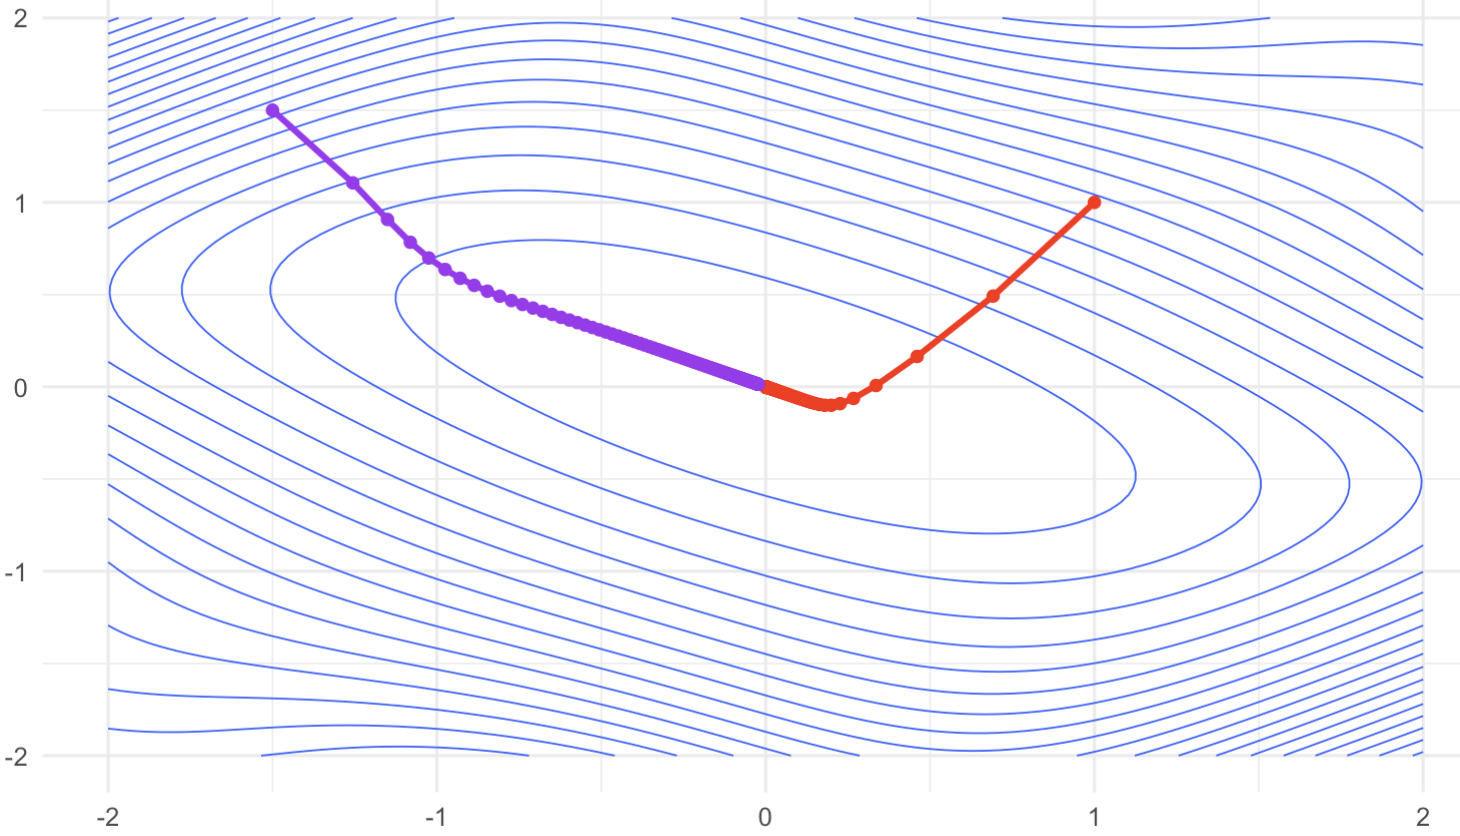
\includegraphics[width=.9\textwidth]{img/gd1.png}}
\end{frame}

%%%%%%%%%%%%%%%%%%%%%%%%%%%%%%%%%%%%%%%%%%%%%%%%%%%%%
\begin{frame}
    \frametitle{Wahl des Startpunkts}
    \begin{itemize}
        \item Konvergenz hängt vom {\bf Startpunkt} ab
          \begin{itemize}
            \item Kann viele Iterationsschritte benötigen
            \item Kann in ein lokales Minimum führen
            \item Kann in einen Sattelpunkt führen (unwahrscheinlich)
        \end{itemize}
    \end{itemize}

    \centerline{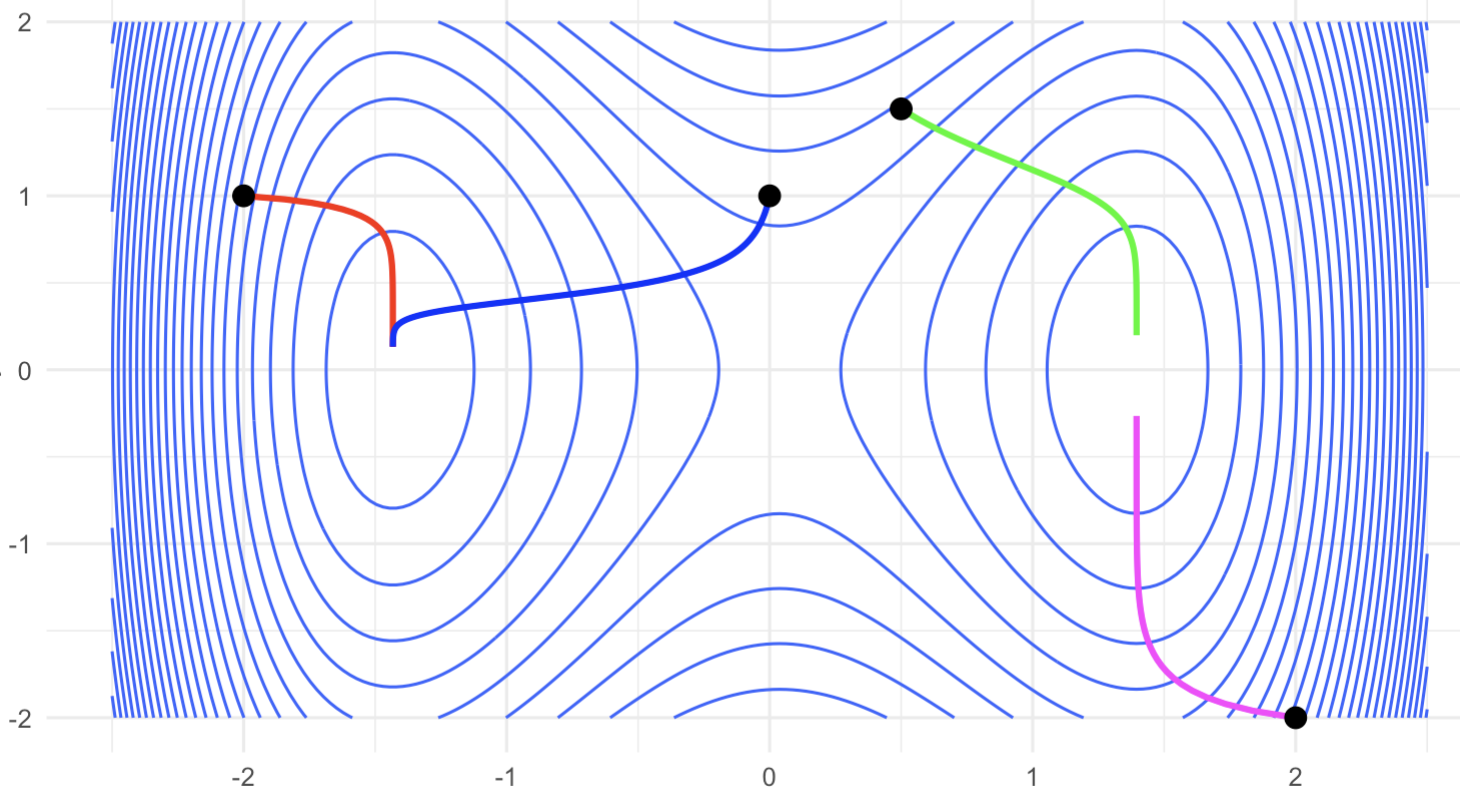
\includegraphics[width=.8\textwidth]{img/gd3.png}}
    \begin{itemize}
        \item Mögliche Strategien: zufällige, mehrfache Startpunkte; benutzen von Vorwissen; ...
    \end{itemize}
\end{frame}



%%%%%%%%%%%%%%%%%%%%%%%%%%%%%%%%%%%%%%%%%%%%%%%%%%%%% 
\begin{frame}
    \frametitle{Lokale und globale Minima}
    \begin{itemize}
        \item GD konvergiert zu einem {\bf lokalen Minimum}!
            \item Lokales Minimum: $f(x) \ge f(x_0)$ für alle $x$ in einer Umgebung von $x_0$.
            \item Globales Minimum: $f(x) \ge f(x_0)$ für alle $x$ im Definitionsbereich.
        \item Meistens suchen wir jedoch das {\bf globale Minimum}
    \end{itemize}
\centerline{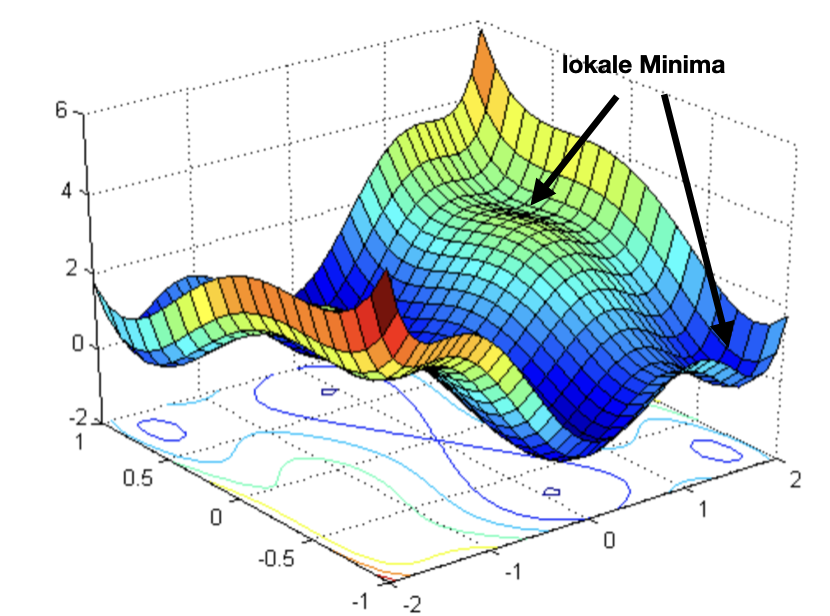
\includegraphics[width=.6\textwidth]{img/local.png}}

\end{frame}


%%%%%%%%%%%%%%%%%%%%%%%%%%%%%%%%%%%%%%%%%%%%%%%%%%%%%
\begin{frame}
    \frametitle{Konvexe Funktionen}
    \begin{itemize}
        \item Eine Funktion $f$ ist {\bf konvex}, wenn für alle $p_1, p_2 \in \mathbb{R}^n$ im Definitionsbereich gilt:
        $$
        f(\lambda p_1 + (1-\lambda)p_2) \leq \lambda f(p_1) + (1-\lambda)f(p_2)~~~~~\forall \lambda \in [0,1]
        $$
        \item anders gesagt: verbindet man 2 Punkte auf der Fläche, dann ist die Verbindungslinie immer oberhalb der Fläche.
        \item Besitzt eine konvexe Funktion ein Minimum, dann ist es immer ein {\bf globales Minimum}: bei den Funktionen funktioniert GD besonders zuverlässig!
        \item Beispiel: $f(x,y) = x^2 + 2y^2$ ist konvex.
    \end{itemize}

\end{frame}

%%%%%%%%%%%%%%%%%%%%%%%%%%%%%%%%%%%%%%%%%%%%%%%%%%%%%
\begin{frame}
    \frametitle{Wahl der Lernrate}
    
    \begin{itemize}
    \item Das Bild der Wanderung hinkt
      \begin{itemize}
      \item Wir folgen dem Gradienten nicht stetig
      \item Wir teleportieren abhängig von der Lernrate
      \end{itemize}
      \only<1>{
        \begin{Denkpause}
          Was kann dadurch schiefgehen?
        \end{Denkpause}
      }
      \pause
    \item Wahl der Lernrate $\eta$ entscheidend
      \begin{itemize}
      \item Zu klein: langsame Konvergenz
      \item Zu groß: divergiert, springt über Minimum
      \end{itemize}
    \end{itemize}
    \centerline{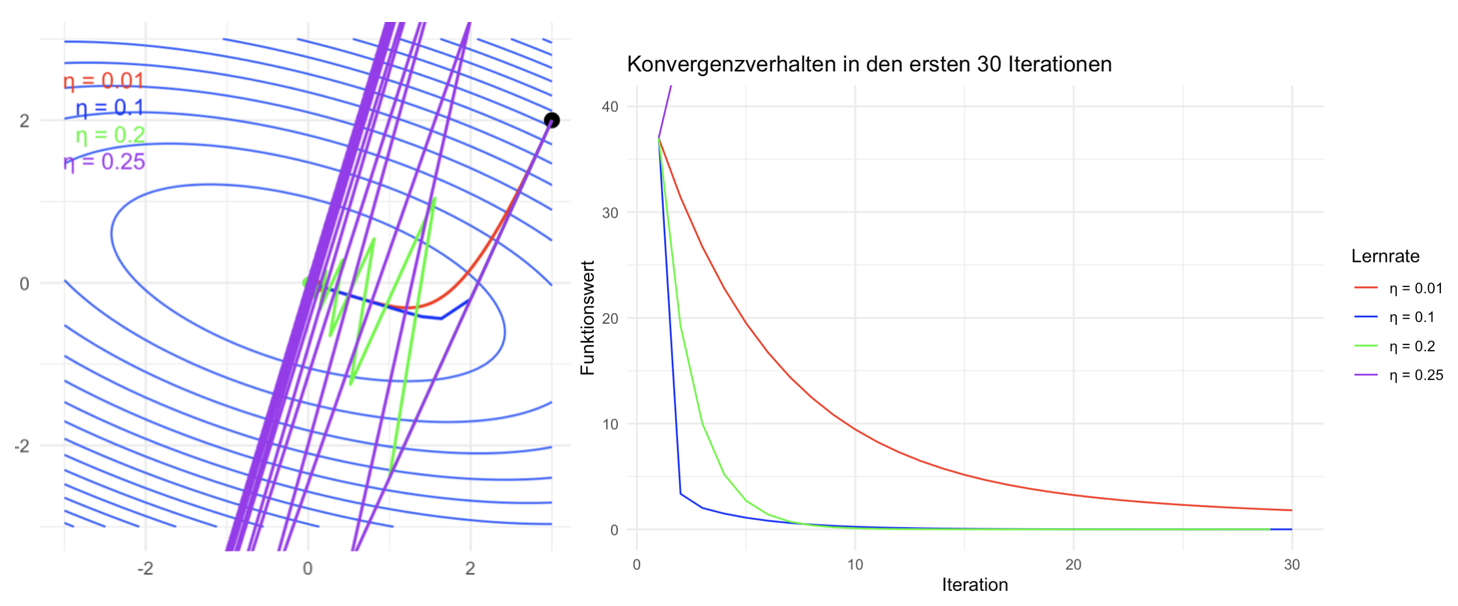
\includegraphics[width=1.1\textwidth]{img/gd4.png}}
\end{frame}

%%%%%%%%%%%%%%%%%%%%%%%%%%%%%%%%%%%%%%%%%%%%%%%%%%%%%
\begin{frame}{Strategien für die Lernrate}
  \begin{itemize}
  \item \glqq{}Schrittweitenhalbierung\grqq{} mit gewählter Grundschrittweite $\eta$
    \begin{enumerate}
    \item Berechne $\vd_n = -\eta\nabla f(\vx_n)$
    \item Berechne $f(\vx_n+\vd_n)$
    \item Ist dieser Wert größer als $f(\vx_n)$, halbiere $\vd_n$ und gehe zu 2.
      \begin{itemize}
      \item Hintergrund: wenn wir minimieren ist es nicht sinnvoll zu
        größeren Werten zu gehen
      \item Achtung! Die Gefahr in einem lokalen Minimum steckenzubleiben wächst
      \end{itemize}
    \end{enumerate}
  \item Line search
    \begin{enumerate}
    \item Betrachte die Funktion $g(t) = f(\vx_n-t\nabla f(\vx_n))$
    \item Finde deren Minimum für $t>0$
      \begin{itemize}
      \item Eindimensionale Minimierung ist einfacher!
      \end{itemize}
      \item Wähle dieses $t$ als Schrittweite $\eta$
    \end{enumerate}
  \end{itemize}
\end{frame}

%%%%%%%%%%%%%%%%%%%%%%%%%%%%%%%%%%%%%%%%%%%%%%%%%%%%%
\begin{frame}
    \frametitle{Anwendungen in der Bioinformatik}

    \begin{itemize}
        \item Proteinfaltungsvorhersage:
        \begin{itemize}
        \item Finden der energetisch günstigsten Konformation
        \item Die Energielandschaft hat viele lokale Minima
        \item Gradientenabstieg mit stochastischen Komponenten
        \end{itemize}
         \item Molekulardynamik-Simulationen:\
        \begin{itemize}
            \item Energieminimierung von Molekülstrukturen
            \item Berechnung stabiler Konformationen von Biomolekülen
        \end{itemize}        
        \item Machine Learning in der Genomik:
        \begin{itemize}
        \item Training von neuronalen Netzen zur Klassifizierung von Tumor-Subtypen anhand von Genexpressionsdaten.
        \item Vorhersage von Protein-Protein-Interaktionen
        \end{itemize}
    \end{itemize}
\end{frame}

%%%%%%%%%%%%%%%%%%%%%%%%%%%%%%%%%%%%%%%%%%%%%%%%%%%%%%%%%%%%
\begin{frame}{Abschlussfragen}
  \begin{enumerate}
  \item Was ist das Prinzip des Abstiegsverfahrens?
  \item Wo liegt das Problem mit lokalen Minima?
  \item Wo liegt das Problem mit der Lernrate?
  \item Wie wählen Sie den Startwert (Startpunkt)?
  \end{enumerate}
\end{frame}


% \input{03a_Flaechen}
%\section{Gewöhnliche Differentialgleichungen}

%%%%%%%%%%%%%%%%%%%%%%%%%%%%%%%%%%%%%%%%%%%%%%%%%%%%%%%%%%%%
%%%%%%%%%%%%%%%%%%%%%%%%%%%%%%%%%%%%%%%%%%%%%%%%%%%%%%%%%%%%
\subsection{Modellierung mit Differentialgleichungen}

\begin{frame}{Ausgangsfragestellung}
  \begin{columns}
    \begin{column}{.6\textwidth}
      \begin{itemize}
      \item<+-> Anzucht von Hefe
      \item<+-> Fermenter
      \item<+-> Fragen:
        \begin{itemize}
        \item<+-> Kann ich für einen beliebigen Zeitpunkt die Anzahl
          an Hefezellen vorhersagen?
        \item<+-> Wie lange muss ich warten, bis ich die gewünschte Ausbeute habe?
        \end{itemize}
      \end{itemize}
    \end{column}
    \begin{column}{.38\textwidth}
      \begin{center}
        \only<2->{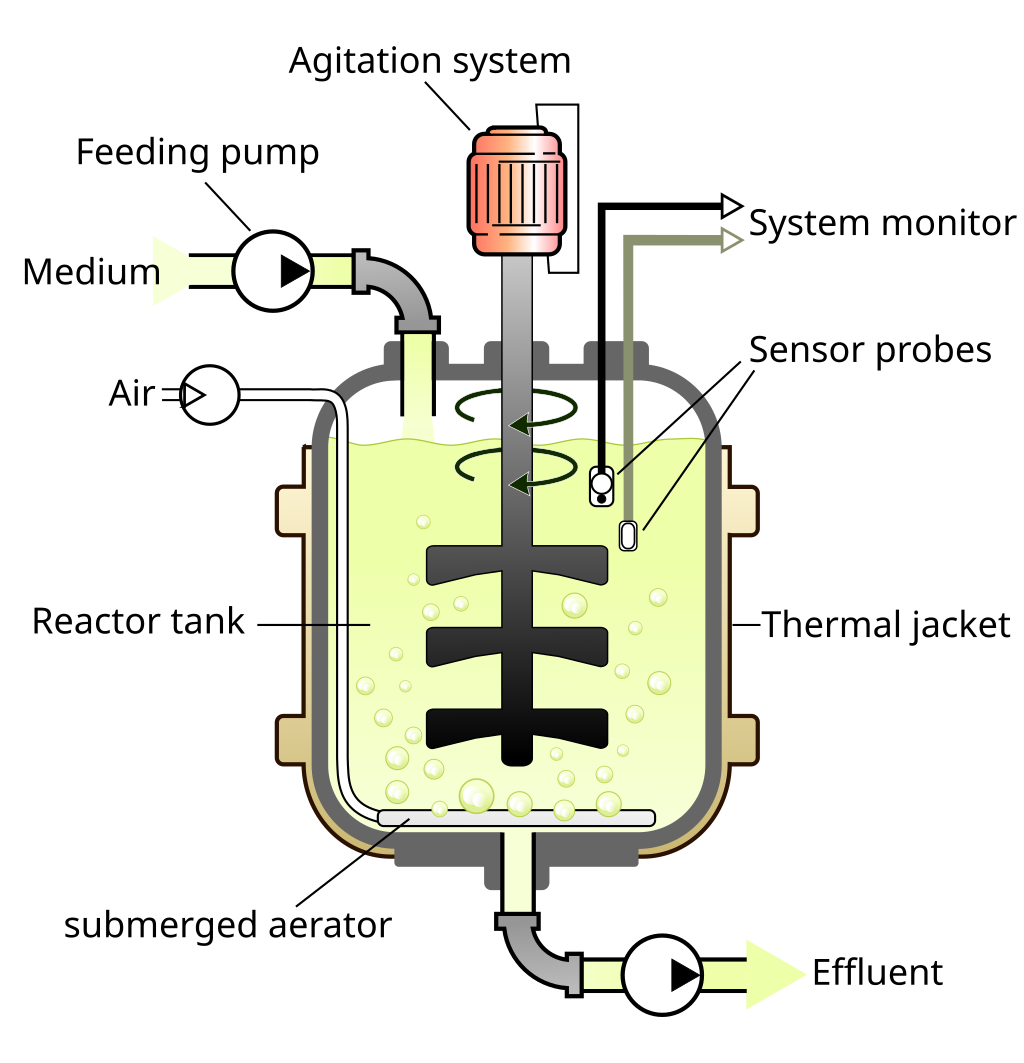
\includegraphics[width=.9\textwidth]{fig/Bioreactor}

          \tiny © Yassine Mrabet, Wikipedia
        }
      \end{center}
    \end{column}
  \end{columns}
\end{frame}

\begin{frame}
  \begin{exampleblock}{Frage}
    Welche Informationen benötigen Sie, um diese Aufgabe zu lösen?
  \end{exampleblock}
\end{frame}

\begin{frame}
  \begin{block}{Verdopplungsrate}
    Under optimal conditions, yeast cells can double their population every 100 minutes.

    \begin{flushright}
      \tiny Wikipedia: Saccaromyces cerevisiæ
    \end{flushright}
  \end{block}

  \pause
  \vspace{5mm}
  
  \begin{tikzpicture}[scale=.9]\footnotesize
    \draw [->] (0,0) -- (12.5,0);
    \draw (0,.1)  -- (0,-.1) node[below] {8:00};
    \draw (2,.1) -- (2,-.1) node[below] {9:40};
    \draw (4,.1) -- (4,-.1) node[below] {11:20};
    \draw (6,.1) -- (6,-.1) node[below] {13:00};
    \draw (8,.1) -- (8,-.1) node[below] {14:40};
    \draw (10,.1) -- (10,-.1) node[below] {16:20};
    \draw (12,.1) -- (12,-.1) node[below] {18:00};
    \only<2>{
      \path (1,.3) node {2x};
      \path (3,.3) node {2x};
      \path (5,.3) node {2x};
      \path (7,.3) node {2x};
      \path (9,.3) node {2x};
      \path (11,.3) node {2x};
    }
    \only<3->{
      \path (0.,.1) node[above,red!60!black]{1000};
      \path (2.,.1) node[above,red!60!black]{2000};
      \path (4.,.1) node[above,red!60!black]{4000};
      \path (6.,.1) node[above,red!60!black]{8000};
      \path (8.,.1) node[above,red!60!black]{16000};
      \path (10.,.1) node[above,red!60!black]{32000};
      \path (12.,.1) node[above,red!60!black]{64000};
    }
    \only<4>{
      \draw[green!45!black] (7,.1) -- (7,-.1) node[below,green!45!black] {13:50};
    }
  \end{tikzpicture}

  \pause
  \vspace{5mm}

  \begin{block}{Anfangspopulation}
    Beispiel: Die Population um 8:00 beträgt 1000 Zellen
  \end{block}
  \pause
  \begin{exampleblock}{Frage}
    Wieviele Zellen haben wir um 13:50?
  \end{exampleblock}
\end{frame}

\begin{frame}{Mathematisch etwas allgemeiner und präziser...}
  \begin{itemize}
  \item Anzahlvariable $N$
  \item Zeitvariable $t$ in Minuten, Startzeit $t_0=8:00$, ``Messzeit'' $T=18:00$
  \item Zeitintervalle $I_k = [t_{k},t_{k+1}]$ der Länge $\Delta t = 100 \text{min}$
    
    \vspace{5mm}
    \hspace*{-1ex}
  \begin{tikzpicture}[scale=.8]\footnotesize
    \draw [->] (0,0) -- (12.5,0);
    \draw (0,.1)  -- (0,-.1) node[below] {8:00};
    \draw (2,.1) -- (2,-.1) node[below] {9:40};
    \draw (4,.1) -- (4,-.1) node[below] {11:20};
    \draw (6,.1) -- (6,-.1) node[below] {13:00};
    \draw (8,.1) -- (8,-.1) node[below] {14:40};
    \draw (10,.1) -- (10,-.1) node[below] {16:20};
    \draw (12,.1) -- (12,-.1) node[below] {18:00};
      \path (0.,.1) node[above,red!60!black]{1000};
      \path (1,.3) node {+1000};
      \path (3,.3) node {+2000};
      \path (5,.3) node {+4000};
      \path (7,.3) node {+8000};
      \path (9,.3) node {+16000};
      \path (11,.3) node {+32000};
    \end{tikzpicture}

    \vspace{5mm}
    
  \item Sei $d_k$ der Zuwachs im Intervall $I_k$
    \begin{gather*}
      N(t_{k+1}) = N(t_k) + d_k,
      \qquad N(T) = N(t_0) + \sum_{k=0}^{n-1} d_k.
    \end{gather*}
  \end{itemize}
  \pause
  \begin{exampleblock}{Frage}
    Im Beispiel ist $d_k=N(t_k)$. Wie ändert sich $d_k$ qualitativ, wenn wir die Intervalle halbieren?
  \end{exampleblock}
\end{frame}

%%%%%%%%%%%%%%%%%%%%%%%%%%%%%%%%%%%%%%%%%%%%%%%%%%%%%%%%%%%%
\begin{frame}{Halbierung der Intervalle}
  \begin{tikzpicture}[scale=3]\footnotesize
    \draw [thick,->] (6.,0) -- (8.5,0);
    \draw (6,.1) node[above] {8000} -- (6,-.1) node[below] {13:00};
    \draw (8,.1) node[above] {16000} -- (8,-.1) node[below] {14:40};
    \path (7,.3) node {+8000};

    \draw [thick,->] (6.,-.7) -- (8.5,-.7);
    \draw (6,-.6) -- (6,-.8) node[below] {13:00};
    \draw (8,-.6) -- (8,-.8) node[below] {14:40};
    \draw (7,-.6) node[above] {\textcolor{red!60!black}{\only<1>{???}\only<3->{11314}}} -- (7,-.8) node[below] {13:50};
    \path (6.5,-.5) node {\textcolor{red!60!black}{\only<1>{+???}\only<3->{3314}}};
    \path (7.5,-.5) node {\textcolor{red!60!black}{\only<1>{+???}\only<3->{4686}}};
  \end{tikzpicture}

  \only<1>{\begin{Denkpause}
      Welche Werte sollten für die Fragezeichen stehen?
    \end{Denkpause}}
  \pause
  \begin{itemize}
  \item Die Summe sollte 8000 ergeben
  \item Der Quotient aus Summand und linkem Wert sollte gleich sein
  \end{itemize}
\end{frame}


\begin{frame}{Lösung von der Intervallänge}
  \begin{itemize}
  \item Es gilt eine Beziehung wie
    $d_k \approx f(t_k)\Delta t$.
  \item Die Funktion $f$ gibt an, wieviele Hefezellen im Zeitintervall
    der Länge $\Delta t$ entstehen
  \item Sie hängt von der aktuellen Anzahl ab
  \item Dann können wir für eine beliebige Folge von $n$ Intervallen
    schreiben
    \begin{gather*}
      N(t_n) = N(t_0) + \sum_{k=0}^{n-1} f(t_k) (\Delta t)_k
    \end{gather*}
    \only<1>{
      \begin{Denkpause}
        Wo haben wir eine solche Modellierung schon gesehen?
      \end{Denkpause}
}
    \pause
    \item Wenn wir die Intervalllänge gegen null gehen lassen, bekommen wir ein Integral
  \end{itemize}
\end{frame}

\begin{frame}
  \begin{itemize}
  \item<+-> Für individuelle Hefezellen ist $\Delta t \to 0$ unsinnig,
    weil sich ab einem Punkt sehr wahrscheinlich keine einzige Zelle
    in einem Intervall vermehrt.
    \item<+-> Wir ersetzen daher die diskrete Anzahl $N(t)$ durch eine
    kontinuierliche Größe $x(t)$ z. B. mit der Einheit Gramm anstelle
    von Stück.
  \end{itemize}
  \begin{block}<+->{Kontinuumshypothese} Wir nehmen an, dass der
    Übergang von einer diskreten zu einer kontinuierlichen Größe keine
    großen Fehler verursacht.
    \begin{itemize}
    \item Die Werte $x \sim N$ und $x\sim N+1$ unterscheiden sich kaum
    \item Statistische Fluktuationen des Zuwachses $d_k$ haben keinen
      merkbaren Einfluss
    \end{itemize}
  \end{block}

  \begin{itemize}
  \item<+-> Hefe: 1 Gramm entspricht $10^9$ Zellen
  \item<+-> Verdopplung entspricht $10^9$ Zellteilungen in 2 Stunden
  \end{itemize}
\end{frame}

\begin{frame}{Integraldarstellung}
  Ersetzen wir $N(t)$ durch $x(t)$ und lassen die Summen konvergieren, so erhalten wir die \textbf{Volterrasche Integralgleichung}
    \begin{gather*}
      x(T) = x(t_0) + \int_{t_0}^T f(t) \dt.      
    \end{gather*}
  \begin{block}{Instantane Reproduktionsrate $R$}
    Für die Funktion unter dem Integral setzen wir
    \begin{gather*}
      f(t) = R x(t).
    \end{gather*}
    Hier repräsentiert $R$ eine Reproduktionsrate für ein unendlich kleines Zeitintervall $dt$.
    %, also
    % \begin{gather*}
    %   R = \lim_{h\to 0} \tfrac{x(t+h)-x(t)}{h}.
    % \end{gather*}
  \end{block}
\end{frame}

\begin{frame}
  Wir erhalten die Darstellung der Funktion $x(t)$ als
  \begin{block}{Volterrasche Integralgleichung}
    \begin{gather*}
      x(t) = x(t_0) + \int_{t_0}^t R x(s) \ds.      
    \end{gather*}    
  \end{block}

  Differenzieren wir auf beiden Seiten ergibt die Darstellung als
  \begin{block}{Differentialgleichung}
    \begin{gather*}
          x'(t) = R x(t)
    \end{gather*}
  \end{block}
\end{frame}

\begin{frame}{Lösungen}
  Aus der Schule ist die Exponentialfunktion bekannt. Es gilt:
  \begin{gather*}
    \tfrac d{dt} e^{Rt} = R e^{Rt}.
  \end{gather*}
  Dies gilt aber auch für alle Funktionen $x(t) = c \,e^{Rt}$ mit einer Konstanten $c$.

  \begin{block}{Anfangswertaufgabe}
    Die Lösungsgesamtheit der Differentialgleichung $x' = Rx$ besteht
    aus allen Funktionen der Form $c\,e^{Rt}$.

    \vspace{1ex}

    Die tatsächliche Lösung erhält man, indem man die Konstante an den Anfangswert $x_0$ angleicht:
    \begin{gather*}
      x_0 = x(t_0) = c e^{Rt_0} \qquad \Rightarrow \qquad c = \frac{x_0}{e^{R t_0}}
    \end{gather*}
  \end{block}
\end{frame}

\begin{frame}{Berechnung von $R$}
  Wenn $\Delta t$ die Zeit zur Verdopplung ist, wie groß ist $R$?
  \begin{itemize}
  \item Wenn $x(0) = x_0$, so gilt $x(T)=2x_0$ nach der Verdopplungszeit
    $T=100 \,\text{min}$
  \item Wir können nun rechnen
    \begin{gather*}
      2 x_0 = x_0 e^{RT}
      \quad\Leftrightarrow\quad
      2 = e^{RT}
      \quad\Leftrightarrow\quad
      \ln 2 = RT
    \end{gather*}
  \item Wir erhalten den Wert
    \begin{gather*}
      R=\frac{\ln 2}{100} \,\text{min}^{-1}  \approx 0.00693 \,\text{min}^{-1}
    \end{gather*}
  \end{itemize}
\end{frame}

\begin{frame}{Einheiten}
  \begin{minipage}{.9\textwidth}
  \begin{itemize}
  \item Wir setzen Einheiten für $t$ und $x$, zum Beispiel
    \begin{gather*}
      t[\text{min}],\qquad x[\text{g}].
    \end{gather*}
  \item Dann hat $x'$ die Einheit $\nicefrac{\text{g}}{\text{min}}$
  \item Wegen
    \begin{gather*}
      R = \frac{x'}{x} \qquad\text{ist die Einheit von $R$ dann}\quad R[\nicefrac1{\text{min}}]
    \end{gather*}
  \end{itemize}    
  \end{minipage}
  \pause
  \begin{block}{Dimensionslose Formulierung}
    Indem man formal durch die Einheiten teilt, werden die Gleichungen
    dimensionslos.

    \vspace{1ex}

    Man kann auch durch charakteristische Größen teilen, um gezielt
    mathematisch einfache Darstellungen zu erhalten.
  \end{block}
\end{frame}

\begin{frame}
  \frametitle<presentation>{Änderung der Einheiten}
  Wir wollen im obigen Beispiel die Zeiteinheit auf Stunden wechseln
  \begin{itemize}
  \item Aus der Beziehung $\ln 2 = RT$ folgt, dass das Produkt der
    Einheiten von $R$ und $T$ einheitenlos sein muss.
  \item Für die Einheiten $T[\text{min}]$ und $R[\text{min}^{-1}]$
    haben wir den Wert von $R$ berechnet.
  \item Wollen wir die Zeiteinheit auf Stunden umrechnen, so müssen
    wir auch den Wert von $R$ mit 60 multiplizieren, also
    \begin{gather*}
      R = \ln 2\frac35\,\text{h}^{-1} \approx 0.416
    \end{gather*}
  \end{itemize}
\end{frame}

\begin{frame}{Charakteristische Zeit}
  \begin{itemize}
  \item Die Verdopplungszeit ist ein Beispiel für eine Charakteristische Zeit
  \item Üblicher: die Zeit, in der die Lösung um den Faktor $e$ zunimmt.
  \item Sei $T$ diese Zeit in irgendeiner Einheit,
    \begin{itemize}
    \item die Zeit mit derselben Einheit $\hat t$,
    \item die dimensionslose Zeit $t= \hat t/T$.
    \end{itemize}
    \pause
  \item Dann gilt für $x(t)$
    \begin{gather*}
      x(1) = x_0 e^{1R} = x_0 e^{R}
    \end{gather*}
    \pause
  \item In dieser Darstellung ist also $R=1$
  \item $R$ ist hier wie $t$ dimensionslos
  \end{itemize}
\end{frame}

%%%%%%%%%%%%%%%%%%%%%%%%%%%%%%%%%%%%%%%%%%%%%%%%%%%%%%%%%%%%%%%%%%%%%%

\begin{frame}
  \only<1>{%
    \begin{Denkpause}
      Was passiert für $t\to\infty$?
    \end{Denkpause}
    
    \begin{Denkpause}
      Was passiert für $t\to\infty$ falls $R<0$?    
    \end{Denkpause}
  }
  \pause
  \begin{itemize}
  \item<+-> Für $R>0$ nimmt die Hefe-Population unbegrenzt und exponentiell zu
    \begin{itemize}
    \item Das ist nicht sehr realistisch
    \end{itemize}
  \item<+-> Für $R<0$ stirbt die Hefe exponentiell aus
  \end{itemize}
\end{frame}

\begin{frame}
  \begin{Denkpause}
    Was erwarten Sie im Fermenter, wenn Sie im Prozess keine Nahrung
    zuführen? Betrachten Sie vor allem den Fall $t\to\infty$.
  \end{Denkpause}

  \begin{Denkpause}
    Was erwarten Sie im Fermenter, wenn Sie im Prozess mit konstanter
    Rate Nahrung zuführen? Betrachten Sie vor allem den Fall
    $t\to\infty$.
  \end{Denkpause}
\end{frame}

\begin{frame}{Modellierung}
  \begin{itemize}
  \item Bisher hatten wir $R$ bei optimalen Bedingungen
    \begin{itemize}
    \item Nahrungsmenge $F_{\text{opt}}$
    \end{itemize}
  \item Bei Nahrungszufuhr $F_{\text{opt}}$ ist der Anteil an verfügbarer Nahrung $1-Vx$
    \begin{itemize}
    \item $V$ der spezifische Verbrauch der Hefe
    \end{itemize}
  \item Jetzt setzen wir unter Vereinfachung für die Reproduktionsrate
    \begin{gather*}
      r = R \frac{F}{F_{\text{opt}}} = R (1-Vx)
    \end{gather*}
  \item Wir erhalten die ``logistische Differentialgleichung''
    \begin{gather*}
      x' = rx = R (1-Vx) x.
    \end{gather*}
  \end{itemize}
\end{frame}

\begin{frame}
  \begin{block}{Lösungen}
    \begin{gather*}
      x_c(t) = \frac{e^{Rt}}{V e^{Rt}+c}
    \end{gather*}
  \end{block}
  \only<1>{
    \begin{Denkpause}
      Glauben Sie mir diese Lösung?
    \end{Denkpause}
  }
  \pause
  \begin{itemize}
  \item Für $t\to\infty$ sind diese Lösungen beschränkt:
    \begin{itemize}
    \item Für $R>0$ konvergiert $x_c(t) \to 1/V$
    \item Für $R<0$ konvergiert $x_c(t) \to 0$
    \end{itemize}
  \end{itemize}
\end{frame}


%%%%%%%%%%%%%%%%%%%%%%%%%%%%%%%%%%%%%%%%%%%%%%%%%%%%%%%%%%%%%%%%%%%%%%
\begin{Abschluss}
\item Wie kann man das Zeitverhalten von Wachstumsprozessen modellieren?
\item Was ist die Kontinuumshypothese?
\item Wie hängen Volterrasche Integralgleichung und Differentialgleichung zusammen?
\item Was ist exponentielles Wachstum?
\item Wie modelliert man Populationsentwicklung bei beschränkten Ressourcen?
\item Wie überprüft man die Lösung einer Differentialgleichung?
\end{Abschluss}
  
%%%%%%%%%%%%%%%%%%%%%%%%%%%%%%%%%%%%%%%%%%%%%%%%%%%%%%%%%%%%%%%%%%%%%% 
%%%%%%%%%%%%%%%%%%%%%%%%%%%%%%%%%%%%%%%%%%%%%%%%%%%%%%%%%%%%%%%%%%%%%%
\subsection{Grundbegriffe}

%%%%%%%%%%%%%%%%%%%%%%%%%%%%%%%%%%%%%%%%%%%%%%%%%%%%%%%%%%%%
\begin{frame}
  \begin{block}{Differentialgleichung}
    Eine Differentialgleichung ist eine Gleichung, die eine Funktion
    und/oder ihre Ableitungen in Beziehung setzt.
  \end{block}
  \begin{columns}
    \begin{column}[t]{.49\textwidth}
      \begin{block}{Gewöhnliche DGl.}
        Es kommen nur Ableitungen bzgl. einer Variablen vor. Beispiel:
        \begin{gather*}
          x^{(3)}(t) + \sin(t) x'(t) = x^2(t) +t^2
        \end{gather*}
      \end{block}
    \end{column}
    \begin{column}[t]{.49\textwidth}
      \begin{block}{Partielle DGl.}
        Es kommen partielle Ableitungen nach mehreren Variablen vor.
        Beispiel:
        \begin{gather*}
          \partial_t u(t,x) - \partial_{xx} u(t,x) = \sin(x)
        \end{gather*}
      [Nicht in dieser Vorlesung]
      \end{block}
    \end{column}
  \end{columns}
  \pause
  \begin{block}{Ordnung einer Differentialgleichung}
    Die Ordnung einer DGl. ist der Grad der höchsten Ableitung, die in
    der Gleichung vorkommt.
  \end{block}
\end{frame}

%%%%%%%%%%%%%%%%%%%%%%%%%%%%%%%%%%%%%%%%%%%%%%%%%%%%%%%%%%%%
\begin{frame}{Systeme gewöhnlicher Differentialgleichungen}
  \begin{itemize}
  \item Ein System gewöhnlicher
    Differentialgleichungen erster Ordnung hat die Form
    \begin{align*}
      x_1'(t) &= f_1\bigl(t,x_1(t),\dots,x_n(t) \bigr)\\
      x_2'(t) &= f_2\bigl(t,x_1(t),\dots,x_n(t) \bigr)\\
      \vdots\\
      x_n'(t) &= f_n\bigl(t,x_1(t),\dots,x_n(t) \bigr)
    \end{align*}
  \item  $n$ ist die Dimension des Systems
  \item Einfacher in Vektorschreibweise
    \begin{gather*}
      \vx'(t) = \vf\bigl(t,\vx(t)\bigr)
    \end{gather*}
  \item Die Funktion $\vx$ beschreibt einen Weg in $\R^n$, auch \textbf{Trajektorie} genannt
  \end{itemize}
\end{frame}

%%%%%%%%%%%%%%%%%%%%%%%%%%%%%%%%%%%%%%%%%%%%%%%%%%%%%%%%%%%%
\begin{frame}
  \begin{itemize}
  \item   Jede Differentialgleichung $n$-ter Ordnung
    \begin{gather*}
      F\bigl(t,x^{(n)},x^{(n-1)},\dots,x',x\bigr) = 0
    \end{gather*}
    lässt sich als System erster Ordnung der Dimension
    $n$ schreiben! Mit $x_1=x$:
    \begin{align*}
      x_1' &= x_2\\
      \vdots\\
      x_{n-1}' &= x_n\\
      F\bigl(t,x_n', x_n,\dots,x_1\bigr)&=0 
    \end{align*}
  \item Durch Auflösen nach $x_n'$ ist die Form
    \begin{gather*}
      \vx' = \vf\bigl(t,\vx\bigr)    
    \end{gather*}
    damit der allgemeine Fall.
    \begin{itemize}
    \item Die Argumente \glqq$t$\grqq{} lassen wir oft weg
    \end{itemize}
  \end{itemize}
\end{frame}

%%%%%%%%%%%%%%%%%%%%%%%%%%%%%%%%%%%%%%%%%%%%%%%%%%%%%%%%%%%%
\begin{frame}
  \begin{block}{Autonome Differentialgleichungen}
    Eine Differentialgleichung heißt autonom, wenn keiner der Terme
    eine explizite Abhängigkeit von der Zeit hat.
  \end{block}
  \begin{columns}
    \begin{column}[t]{.49\textwidth}
      \begin{block}{Autonom}
        \begin{gather*}
          \vx' = \vf(\vx)
        \end{gather*}
      \end{block}
    \end{column}
    \begin{column}[t]{.49\textwidth}
      \begin{block}{Nicht autonom}
        \begin{gather*}
          \vx' = \vf(t,\vx)
        \end{gather*}
      \end{block}
    \end{column}
  \end{columns}
  \pause
  \begin{Denkpause}
    Welche Prozesse führen zu autonomen DGln., welche zu nicht autonomen?
  \end{Denkpause}
\end{frame}

%%%%%%%%%%%%%%%%%%%%%%%%%%%%%%%%%%%%%%%%%%%%%%%%%%%%%%%%%%%%
\begin{frame}
  \frametitle<presentation>{Modellierung mit autonomen Dgln.}
  \begin{itemize}
  \item Annahme: Zeitinvarianz,  konstante äußere Bedingungen
    \begin{itemize}
    \item Naturgesetze
    \item Temperatur
    \item Nährstoffzufuhr
    \item pH-Wert
    \item etc.
    \end{itemize}
  \item Beispiele: Reaktionsnetzwerke, metabolische Dynamik
  \item Bei autonomen DGln. ist der Startzeitpunkt frei
  verschiebbar, wir wählen oft $t_0 = 0$.
  \end{itemize}
\end{frame}


%%%%%%%%%%%%%%%%%%%%%%%%%%%%%%%%%%%%%%%%%%%%%%%%%%%%%%%%%%%%
\begin{Abschluss}
\item Was ist die Ordnung einer Differentialgleichung?
\item Was sind Systeme von Dgln.?
\item Welche Darstellung genügt?
\item Wie zeichnen sich autonome Dgln. aus?
\end{Abschluss}


%%%%%%%%%%%%%%%%%%%%%%%%%%%%%%%%%%%%%%%%%%%%%%%%%%%%%%%%%%%%
%%%%%%%%%%%%%%%%%%%%%%%%%%%%%%%%%%%%%%%%%%%%%%%%%%%%%%%%%%%%
\subsection{Richtungsfelder und Fixpunkte}

\begin{frame}{Richtungsfelder}
  \begin{itemize}
  \item Die Lösung $x(t)$ einer Differentialgleichung kann als Weg
    $(t,x(t))$ dargestellt werden
  \item Der Geschwindigkeitsvektor beschreibt die Änderung
    in der Zeit:
    \begin{gather*}
      \begin{pmatrix}
        t'\\x'(t)
      \end{pmatrix}
      =
      \begin{pmatrix}
        1\\f(t,x)
      \end{pmatrix}
    \end{gather*}
  \item Zu jedem Punkt in der $(t,x)$-Ebene ist ein solcher Vektor
    durch die Differentialgleichung gegeben
  \item Dieses \textbf{Richtungsfeld} erlaubt die graphische
    Rekonstruktion der Lösung $x(t)$
  \end{itemize}
\end{frame}

\begin{frame}{Richtungsfeld der logistischen Dgl.}
  \begin{columns}
    \begin{column}[t]{.2\textwidth}
    \begin{gather*}
      x'= (1-x) x
    \end{gather*}
    \begin{exampleblock}{Frage}
      Verhalten für $t\to\infty$
    \end{exampleblock}
    \end{column}
    \begin{column}[t]{.78\textwidth}
      \mbox{}
      
      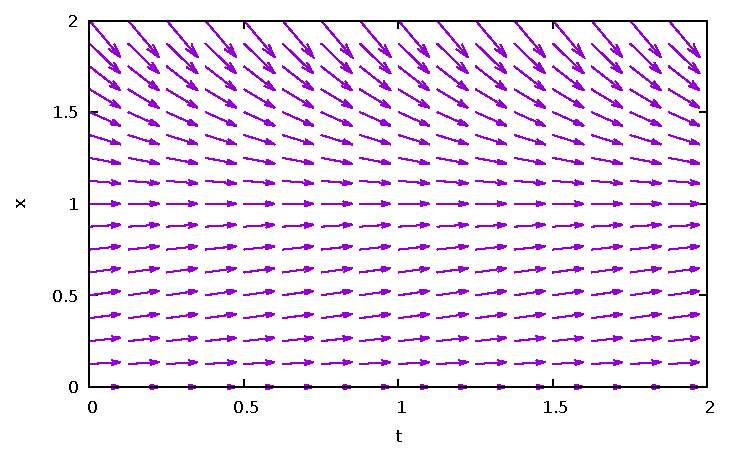
\includegraphics[width=\textwidth]{gnuplot/logistic.pdf}
    \end{column}
  \end{columns}
\end{frame}

\begin{frame}
  \frametitle<presentation>{Negative Startwerte}
  \begin{columns}
    \begin{column}[t]{.2\textwidth}
    \begin{gather*}
      x'= (1-x) x
    \end{gather*}      
    \end{column}
    \begin{column}[t]{.78\textwidth}
      \mbox{}
      
      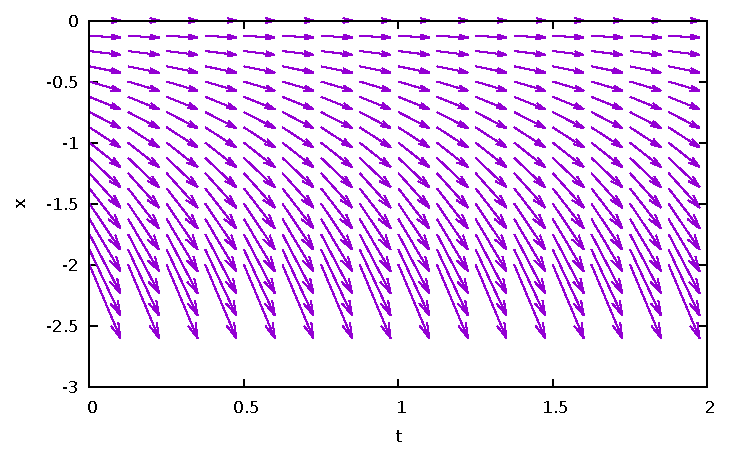
\includegraphics[width=\textwidth]{gnuplot/logisticm.pdf}
    \end{column}
  \end{columns}
\end{frame}

%%%%%%%%%%%%%%%%%%%%%%%%%%%%%%%%%%%%%%%%%%%%%%%%%%%%%%%%%%%%
\begin{frame}{Weiteres Beispiel Richtungsfeld}
  \includegraphics[width=.8\textwidth]{gnuplot/sinelog.pdf}
  \only<1>{\begin{Denkpause}
      Was unterscheidet dieses Richtungsfeld vom vorherigen?
      
      Was für einen anderen Gleichungtyp zeigt es?
    \end{Denkpause}}
  \pause
  \begin{itemize}
  \item Keine autonome Gleichung, Richtung hängt von $t$ ab
  \end{itemize}
\end{frame}

\begin{frame}{Fixpunkte}
  \begin{itemize}
  \item Für autonome Gleichungen/Systeme sind Fixpunkte von hoher Bedeutung
  \item Fixpunkte entsprechen Gleichgewichtszuständen
  \item Es gilt:
    \begin{gather*}
      x'(T) = 0 \qquad \Rightarrow \qquad x'(t) = 0
      \quad\text{für alle}\quad t>T
    \end{gather*}
    \item Alle Nullstellen von $f(x)$ sind Fixpunkte
  \end{itemize}
\end{frame}

\begin{frame}{Eigenschaften von Fixpunkten}
  Fixpunkt $\vx_0$
  \begin{itemize}
  \item Anziehend: für einen Startwert $\vx$ nah am Fixpunkt gilt
    \begin{gather*}
      \vx\to\vx_0\quad\text{wenn}\quad t\to\infty
    \end{gather*}
    \begin{itemize}
    \item stabiles Gleichgewicht
    \item ist ein System im Gleichgewicht und wird gestört, so
      kehrt es in dasselbe Gleichgewicht zurück
    \end{itemize}
  \item Absto\ss{}end: für einen Startwert $\vx\neq\vx_0$ bewegt sich
    die Trajektorie von $\vx_0$ weg
    \begin{itemize}
    \item instabiles Gleichgewicht
    \end{itemize}
  \item Wir werden weitere Arten von Fixpunkten kennenlernen
  \end{itemize}
\end{frame}

\begin{frame}{Fixpunkte bei Gleichungen}
  \begin{columns}
    \begin{column}{.08\textwidth}
      \mbox{}
      
      \begin{tikzpicture}[scale=1.]]
        \node (A) at (0,0) {$\bullet$};
        \node (B) at (0,1) {$\bullet$};
        \node (C) at (0,-2) {};
        \node (D) at (0,3) {};

        \draw[thick,-Stealth] (A) edge (B);
        \draw[thick,-Stealth] (A) edge (C);
        \draw[thick,-Stealth] (D) edge (B);
      \end{tikzpicture}
    \end{column}
    \begin{column}{.9\textwidth}
      \only<1>{Bei autonomen Gleichungen genügt ein eindimensionaler
        Strahl mit Richtungspfeilen}
      \only<2->{
      \begin{itemize}
      \item anziehende Fixpunkte: Richtungspfeile zeigen zum Fixpunkt hin
        \begin{xalignat*}3
          x&>x_0 &\Rightarrow&&f(x)&<0\\
          x&<x_0 &\Rightarrow&&f(x)&>0
        \end{xalignat*}
      \item abstoßende Fixpunkte: Richtungspfeile zeigen vom Fixpunkt weg
        \begin{xalignat*}3
          x&>x_0 &\Rightarrow&&f(x)&>0\\
          x&<x_0 &\Rightarrow&&f(x)&<0
        \end{xalignat*}
      \item gemischte Fixpunkte
      \end{itemize}
      }
    \end{column}
  \end{columns}
\end{frame}

 \begin{frame}{Beispiel}
   \begin{gather*}
     f(x) = x^2(x-1)(x+1)
   \end{gather*}
   \begin{columns}
     \begin{column}{.08\textwidth}
       \mbox{}
       \only<2->{
         \begin{tikzpicture}[scale=1.]]
           \node (A) at (0,0) {$\bullet$};
           \node (B1) at (0,1) {$\bullet$};
           \node (B2) at (0,-1) {$\bullet$};
           \node (C) at (0,-3) {};
           \node (D) at (0,3) {};

           \draw[thick,-Stealth] (C) edge (B2);
           \draw[thick,-Stealth] (B1) edge (D);
           \draw[thick,-Stealth] (A) edge (B2);
           \draw[thick,-Stealth] (B1) edge (A);
         \end{tikzpicture}}
     \end{column}
     \begin{column}{.9\textwidth}
       \begin{itemize}
       \item Die Funktion hat die Nullstellen $x=-1,0,1$
       \item Ihre Vorzeichen sind
         \begin{gather*}
           \begin{array}{r@{\quad}l}
             + & x<-1\\
             - & -1 < x < 0\\
        - & 0 < x < 1 \\
             + & 1 < x
           \end{array}
         \end{gather*}
       \item<3-> Es ist also $-1$ in anziehender, $1$ ein
         absto\ss{}ender und 0 ein gemischter Fixpunkt
       \end{itemize}
     \end{column}
   \end{columns}
 \end{frame}
 
 \begin{Abschluss}
 \item Was können wir an Richtungsfeldern ablesen?
 \item Wie unterscheiden sich die Richtungsfelder autonomer und
   nicht autonomer Gleichungen?
 \item Was ist die Bedeutung von Fixpunkten?
 \item Welche Typen von Fixpunkten haben wir kennengelernt?
 \end{Abschluss}
 
%%%%%%%%%%%%%%%%%%%%%%%%%%%%%%%%%%%%%%%%%%%%%%%%%%%%%%%%%%%%%%%%%%%%%% 
%%%%%%%%%%%%%%%%%%%%%%%%%%%%%%%%%%%%%%%%%%%%%%%%%%%%%%%%%%%%%%%%%%%%%%
\subsection{Systeme von Differentialgleichungen}

\begin{frame}{Erweiterung auf zweite Komponente}
  Modellannahmen
  \begin{itemize}
  \item Sardinen finden optimale Nahrung und werden von
    Thunfischen gefressen
  \item Thunfisch frisst Sardinen und stirbt eines natürlichen
    Todes
  \end{itemize}
  \pause
  Wir wollen möglichst einfache Beziehungen annehmen!
  \begin{exampleblock}{Aufgabe}
    Überlegen Sie sich, wie Sie die Entwicklung der Populationen
    modellieren könnten!
  \end{exampleblock}
\end{frame}

\begin{frame}{Modellierung}
  \begin{itemize}
  \item<+-> Sardinen $x$:
    \begin{itemize}
    \item Vermehrung mit fester Rate: $ax$
    \item Verringerung abhängig vom Thunfisch: $-bxy$
    \end{itemize}
    \begin{gather*}
      x' = ax-bxy
    \end{gather*}
  \item<+-> Thunfisch $y$:
    \begin{itemize}
    \item Feste Sterberate: $-cy$
    \item Vermehrung abhängig von Sardinen: $dxy$
    \end{itemize}
    \begin{gather*}
      y' = -cy + dxy
    \end{gather*}
  \item<+-> $a,b,c,d$ sind angenommene, feste Parameter
  \end{itemize}
\end{frame}

\begin{frame}{Lotka-Volterra-Gleichungen}
  \begin{gather*}
    \begin{aligned}
      x' &=& ax &-bxy\\
      y' &=& -cy & +dxy
    \end{aligned}
  \end{gather*}

  Autonomes System der Dimension zwei
  \begin{itemize}
  \item[$\Rightarrow$] die Entwicklung hängt nur von $(x,y)$ ab 
  \end{itemize}

  \begin{block}{Dynamische Systeme}
    Ein solches System von Differentialgleichungen ist ein besonderer
    Fall eines dynamischen Systems. Wir werden im Folgenden Argumente
    zur Untersuchung dynamischer Systeme auf dieses System anwenden.
  \end{block}
\end{frame}

\begin{frame}{Phasenraumdiagramme}
  \begin{itemize}
  \item Man bezeichnet den Raum der möglichen Zustände $(x,y)$ als Phasenraum
  \item Die Abbildung $t\mapsto(x(t),y(t))$ ist ein Weg im Phasenraum
  \item Sein Geschwindigkeitsvektor $(x',y')$ ist die rechte Seite der Dgl.
  \item Wieder können wir Richtungsfelder zeichnen
    \begin{itemize}
    \item In jedem Punkt $(x,y)$ hängt der Geschwindigkeitsvektor von $x$ und $y$ ab
    \item Die Vektoren sind immer tangential zur Lösungskurve
    \item In diesem Bild gibt es keine Zeit (Kurve!)
    \end{itemize}
  \end{itemize}
\end{frame}

\begin{frame}{Richtungsfeld im Phasenraum}
  \begin{center}
    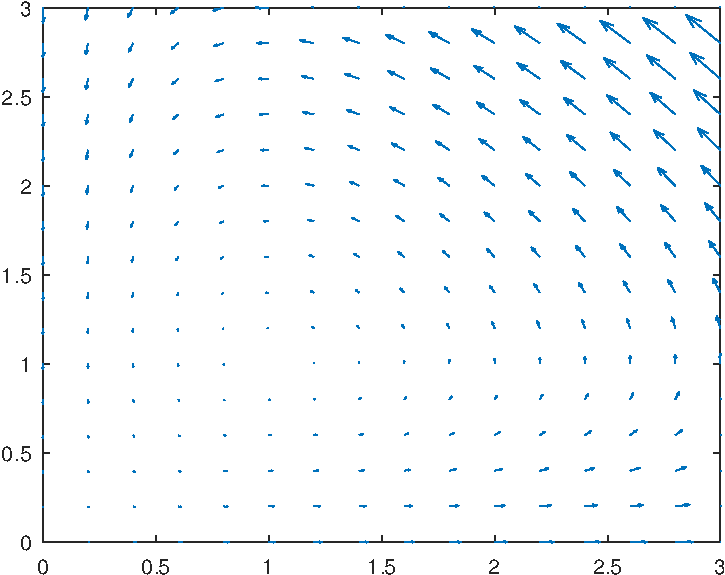
\includegraphics[width=.7\textwidth]{octave/volterra-vectors-crop.pdf}
  \end{center}
\end{frame}

\begin{frame}{Lösung im Phasenraum}
  \begin{center}
    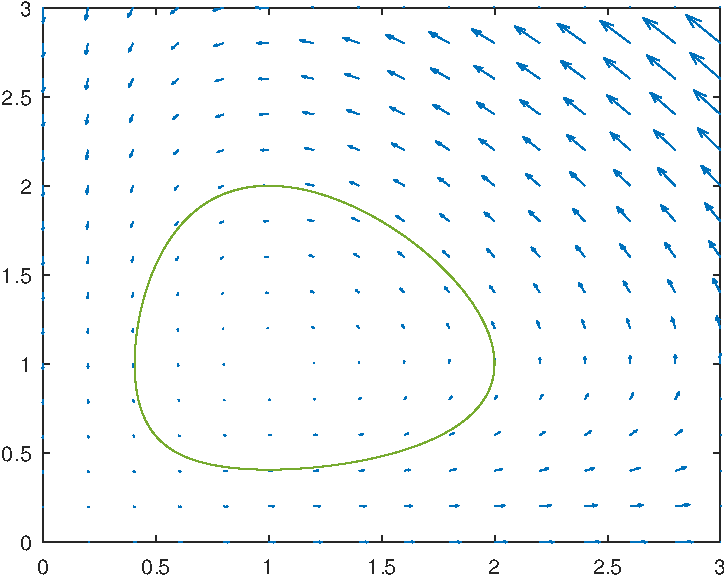
\includegraphics[width=.7\textwidth]{octave/volterra-phasespace-crop.pdf}
  \end{center}
  Eine als Beispiel berechnete Lösungskurve
\end{frame}

\begin{frame}{Lösung als Funktion der Zeit}
  \begin{center}
    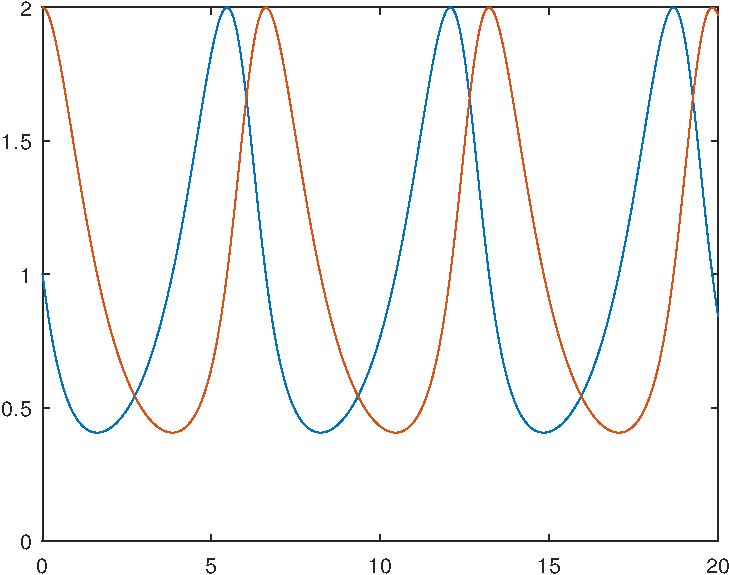
\includegraphics[width=.7\textwidth]{octave/volterra-timeseries-crop.pdf}
  \end{center}
  Die Lösung als Weg: was ist $x$, was ist $y$?
\end{frame}

\begin{frame}{Fixpunkte}
  \only<1>{
    \begin{Denkpause}
      Gibt es Fixpunkte?
    \end{Denkpause}
  }
  \pause
  \begin{itemize}
  \item Fixpunkte des Systems sind Nullstellen der rechten Seite
    \begin{gather*}
      \begin{aligned}
        x' &=& ax &-bxy\\
        y' &=& -cy & +dxy
      \end{aligned}
    \end{gather*}
  \item Offensichtlich ist $(0,0)$ ein Fixpunkt
    \begin{itemize}
    \item Es gibt keine Individuen, die sich vermehren könnten
    \end{itemize}
    \pause
  \item Ein zweiter Fixpunkt ist
    \begin{gather*}
      x=\frac cd,\qquad y=\frac ab
    \end{gather*}
    \begin{itemize}
    \item Tunfisch und Sardinen sind im Gleichgewicht
    \end{itemize}
  \end{itemize}
\end{frame}

\begin{frame}{Erhaltungssätze}
  \begin{itemize}
  \item Wir führen die folgende Größe ein:
    \begin{gather*}
      V(x,y) = dx - c \ln x + by - a \ln y
    \end{gather*}
  \item Für jede Lösung der Lotka-Volterra-Gleichungen $(x(t),y(t))$ gilt
    \begin{gather*}
      d_t V\bigl(x(t),y(t)\bigr) = 0
    \end{gather*}
    \pause
  \item Eine solche Aussage nennt man \textbf{Erhaltungssatz}, $V$
    nennt man eine \textbf{Erhaltungsgröße}
  \item Erhaltungsgrößen spielen eine wichtige Rolle für das
    Verständnis von dynamischen Systemen
  \item Mit Ihnen zeigt man Eigenschaften von Lösungen, z.B.
    \begin{itemize}
    \item beschränkt
    \item periodisch
    \end{itemize}
  \end{itemize}
  
\end{frame}

\begin{Aufgabe}
  Zeigen Sie, dass die Erhaltungsgleichung
  $d_t V\bigl(x(t),y(t)\bigr) = 0$ tatsächlich für jede Lösung der Lotka-Volterra-Gleichungen $(x(t),y(t))$ gilt.
\end{Aufgabe}

\begin{frame}
  \begin{block}{Warnung}
    Für die Lotka-Volterra-Gleichungen gibt es keine geschlossene
    Darstellung der Lösungen.
  \end{block}

  Es lassen sich aber einige Aussagen treffen
  \begin{itemize}
  \item Es gibt die beiden Fixpunkte $(0,0)^T$ und
    $\left(\tfrac cd,\tfrac ab\right)^T$
  \item Es gibt Erhaltungssätze
  \item Lösungen sind periodisch
  \end{itemize}
\end{frame}

\begin{frame}{Lösungen zu verschiedenen Anfangswerten}
  \begin{center}
    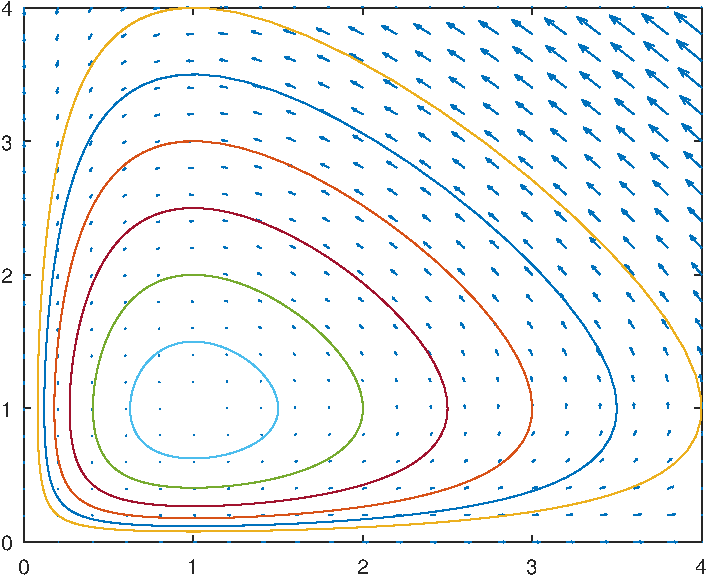
\includegraphics[width=.7\textwidth]{octave/volterra-multi-crop.pdf}
  \end{center}    
\end{frame}

\begin{frame}{Ideen zur Steuerung des Systems}
  Aufgabe: Sie wollen durch das Abfischen von Tunfisch die Sardinenpopulation erhöhen
  \begin{itemize}
  \item Wird das jederzeit funktionieren?
  \visible<3->{
    \begin{itemize}
    \item Es ist die Kenntnis der relativen Position zum Fixpunkt nötig, um gezielt zu steuern.
    \end{itemize}
  }
  \item Kann es langfristig Erfolg haben?
  \visible<4->{
    \begin{itemize}
    \item Langfristig wird das System um denselben Fixpunkt oszillieren
    \end{itemize}
  }
  \end{itemize}
  \visible<2>{
    \begin{Denkpause}
      Argumentieren Sie anhand der vorherigen Grafik
    \end{Denkpause}
  }
  \visible<5>{
    \begin{block}{}
      Wir haben soeben einen ersten Einblick in die Steuerung dynamischer Systeme gewonnen
    \end{block}
  }
\end{frame}

\begin{onlyenv}<article>
  \begin{envgkerror}{Ausarbeiten}
    \begin{Aufgabe}
      \begin{enumerate}
      \item Modifizieren Sie die Lotka-Volterra-Gleichungen für den
        Fall, dass Tunfische mit einer Rate $ey$ gefangen werden.
      \item Finden Sie Fixpunkte der modifizierten Gleichungen
      \item Skizzieren Sie das zugehörige Vektorfeld
      \end{enumerate}
    \end{Aufgabe}
  \end{envgkerror}
\end{onlyenv}

\begin{Abschluss}
\item Was wird im Phasenraumdiagramm dargestellt?
\item Welcher Bezug besteht zwischen Vektorfeld und der Kurve einer Lösung?
\item Wie erkennen Sie stationäre Punkte?
\item Wie erkennen Sie die Auswirkung von Eingriffen in das System?
\end{Abschluss}

%%%%%%%%%%%%%%%%%%%%%%%%%%%%%%%%%%%%%%%%%%%%%%%%%%%%%%%%%%%%%%%%%%%%%%
%%%%%%%%%%%%%%%%%%%%%%%%%%%%%%%%%%%%%%%%%%%%%%%%%%%%%%%%%%%%%%%%%%%%%%
\subsection{Kompartimentmodelle in der Epidemiologie}

\begin{frame}{Kompartimentmodelle}
  \begin{itemize}
  \item Komplexe Verhältnisse werden durch wenige diskrete \glqq{}Kompartimente\grqq{} (compartments) ersetzt
    \begin{itemize}
    \item Personengruppen in der Epidemiologie
    \item Regionen in Zellen
    \end{itemize}
  \item Jedes der Kompartimente wird homogen angenommen
    \begin{itemize}
    \item Bzgl. des Modell gleiche Eigenschaften
    \item Vollständige Durchmischung
    \item Epidemiologie: keine räumliche Auflösung
    \end{itemize}
  \item Der Austausch zwischen den Gruppen ist homogen
    \begin{itemize}
    \item Epidemiologie: die Wahrscheinlichkeit, jemanden aus einer
      der Gruppen zu treffen ist gleich
    \item Das zusammentreffen von Personen ist zeitlich homogen
    \end{itemize}
  \end{itemize}
\end{frame}

\begin{frame}{Das SIR-Modell}
  Drei Personengruppen mit konstanter Gesamtzahl $N$
  \begin{gather*}
    N = S+I+R
  \end{gather*}
  \begin{description}
  \item[Susceptible] $S$ Personen, die sich anstecken können
  \item[Infectious] $I$ infizierte Personen, die die Krankheit weitergeben können
  \item[Removed] $R$ Personen, die nach der Erkrankung immun sind
  \end{description}
  \pause
  \begin{block}{Ethische Komponente}
    In diesen Modellen werden Personen nicht mehr als Menschen
    betrachtet, sondern als komponenten in einem mathematischen
    System. So nützlich Modelle dieser Art sind, so sind sie doch
    prinzipiell nicht mit §1 GG verträglich. Das muss bei ihrer
    Anwendung immer berücksichtigt werden.
  \end{block}
\end{frame}

\begin{frame}{Übergänge zwischen den Gruppen}
  \begin{description}
  \item[$S\to I$] Eine Person $S$ trifft eine infektiöse Person $I$ und wird mit
    der Wahrscheinlichkeit $\hat \beta$ infiziert.
    \begin{itemize}
    \item Personen treffen kontinuierlich andere Personen mit der Rate $m$ pro Zeiteinheit
    \item Die Wahrscheinlichkeit, dass die andere Person infektiös ist, ist $I/N$.
    \end{itemize}
  \item[$I\to R$] Eine infizierte Person erholt sich oder stirbt mit
    einer Rate $\gamma$ pro Zeiteinheit
  \end{description}
  \pause Anmerkung: $\hat\beta$ ist die Übertragungswahrscheinlichkeit
  einer Begegnung. Wir machen die Annahme, dass die Übertragungsrate
  linear mit der Anzahl der Begegnunen wächst und setzen
  $\beta = m \hat\beta$. Auf diese Art sind alle Parameter bezüglich
  derselben Zeiteinheit, typischerweise Tage.
\end{frame}

\begin{frame}{Die Gleichungen}
  \begin{block}{In der Einheit \glqq{}Personen\grqq{}}

    \only<presentation>{\vspace*{-2ex}}
    \begin{align*}
      d_t S &=-\beta S\frac IN\\
      d_t I &=\beta S\frac IN - \gamma I\\
      d_t R &=\gamma I
    \end{align*}  
  \end{block}

  \begin{onlyenv}<article> Die Gleichungen in der Einheit Personen
    sind mathematisch unhandlich, auch wenn die Ergebnisse sofort
    anwendbar sind. Eleganter ist die Darstellung un
    Bevölkerungsanteilen, indem jede Größe durch $N$ dividiert
    wird. Da damit auch die Ableitung entsprechend dividiert wird,
    werden die Gleichungen unabhängig von $N$ und gelten für beliebige
    Bevölgerungen.
  \end{onlyenv}
  \begin{block}{In der Einheit \glqq{}Bevölkerungsanteil\grqq{}}
    \only<presentation>{\vspace*{-2ex}}
    \begin{align*}
      d_t S &=-\beta SI\\
      d_t I &=\beta SI - \gamma I\\
      d_t R &=\gamma I
    \end{align*}  
  \end{block}
\end{frame}

\begin{frame}{Eigenschaften der Lösung}
  \begin{align*}
    d_t S &=-\beta SI\\
    d_t I &=\beta SI - \gamma I\\
    d_t R &=\gamma I
  \end{align*}  
  \begin{itemize}
  \item Alle Größen liegen im Intervall $[0,1]$
    \begin{itemize}
    \item Folgt aus dem Ansatz als Bevölkerungsanteil
    \item Muss für Lösungen überprüft werden
    \end{itemize}
  \item $S$ ist monoton fallend und $R$ steigend
    \begin{itemize}
    \item Daher konvergieren beide für $t\to\infty$
    \end{itemize}
  \item Jeder Punkt $(S,0,R)$ ist ein Fixpunkt
  \end{itemize}
\end{frame}

\begin{frame}{Reproduktionszahlen}
  \begin{gather*}
    d_t I = \beta SI-\gamma I = (R_0S-1) \gamma I
  \end{gather*}
  \begin{block}{Basisreproduktionszahl $R_0$}
    $R_0$ gibt an, wieviele Personen von einer infektiösen Person
    angesteckt werden, wenn $S\approx 1$, also zu Beginn der
    Epidemie. Sie ergibt sich als
    \begin{gather*}
      R_0 = \frac\beta\gamma
    \end{gather*}
  \end{block}

  \begin{block}{Effektive Reproduktionszahl $R_e$}
    $R_e = SR_0$ gibt an, wieviele Personen im Verlauf der Epidemie
    von einer infektiösen Person angesteckt werden.
  \end{block}
\end{frame}

\begin{frame}
  \frametitle<presentation>{Entwicklung von $I$}
  \begin{gather*}
    d_t I = (R_e-1) \gamma I
  \end{gather*}
  \begin{description}
  \item[$R_e>1$] Die Anzahl der Infektiösen wächst
    \begin{itemize}
    \item Für $R_0>1$ beginnt die Epidemie mit exponentiellem Wachstum
    \item Dies wird gebremst, wenn $S$ deutlich unter 1 liegt
    \end{itemize}
  \item[$R_e<1$] Die Anzahl der Infektiösen schrumpft
    \begin{itemize}
    \item Für $R_0<1$ bricht keine Epidemie aus
    \item Im Endstadium schrumpft die Zahl der Infektiösen exponenziell
    \end{itemize}
  \item[$R_e=1$] Grenzfall $d_t I = 0$
    \begin{itemize}
    \item Falls $I>0$, ist $S$ streng monoton fallend, es ist also kein Fixpunkt
    \item Eintritt der \glqq{}Herdenimmunität\grqq{}
    \end{itemize}
  \end{description}
\end{frame}

\begin{frame}{Der Grenzwert für unendliche Zeit}
  \begin{itemize}
  \item Wir haben bereits gesehen:
    \begin{itemize}
    \item $I\to 0$ wenn $t\to \infty$
    \item Die Grenzwerte $S_\infty$ und $R_\infty$ existieren 
    \end{itemize}
  \item Es gilt dann $S_\infty+R_\infty = 1$
  \item Aufwändige mathematische Berechnungen ergeben
    \begin{gather*}
      S_\infty = e^{R_0(S_\infty-1)}
    \end{gather*}
    \begin{itemize}
    \item Beispiel für $R_0=3$ ist $S_\infty \approx 5.95\%$
    \end{itemize}
  \end{itemize}
\end{frame}

\begin{Aufgabe}
  \begin{enumerate}
  \item Modifizieren Sie das SIR-Modell, so dass die Immunität der Gruppe
  $R$ exponentiell abklingt.
  \item Welche Grundannahmen der Analyse für $t\to\infty$ ändern sich dadurch?
  \end{enumerate}
\end{Aufgabe}

\begin{frame}{Das SEIR-Modell}
  \begin{itemize}
  \item Modellierung von Inkubationszeiten
  \item Zusätzlich zum SIR-Modell fügen wir eine weitere Gruppe hinzu
    \begin{itemize}
    \item $E$ (exposed) Infiziert, aber (noch) nicht infektiös
    \end{itemize}
  \item Es gibt eine Übergangsrate $\sigma$ von $E$ nach $I$
  \end{itemize}
  \begin{align*}
    d_t S &=-\beta SI\\
    {\color{blue}d_t E} &{\color{blue}=\beta SI - \sigma E}\\
    d_t I &={\color{blue}\sigma E} - \gamma I\\
    d_t R &=\gamma I
  \end{align*}  
\end{frame}

\begin{frame}{Schwächen der Modelle}
  Im Plenum möchte ich gern diskutieren, wo bei den SIR- und
  SEIR-Modellen eine fundamentale Schwäche liegt und wie man sie
  beheben sollte.
\end{frame}

\begin{frame}{Was ist ein mathematisches Modell}
  \begin{itemize}
  \item Es ist ein System von mathematischen Formeln, das den
    modellierten Prozess mit einer für die Anwendung hinreichenden
    Genauigkeit beschreibt
  \item Es ist eine Abstraktion und damit Vereinfachung
  \item Es beruht auf expliziten Annahmen und erlaubt Schlüsse aus diesen
  \item Es ist in dem Sinne überprüfbar, dass Messwerte und Rechnungen
    hinreichend nah beieinander liegen
  \item Es ist \textbf{nicht} eine wahre oder falsche Aussage über die Natur
  \end{itemize}
\end{frame}

\begin{Abschluss}
\item Was ist ein Kompartimentmodell?
\item Wie modellieren Sie die \glqq{}Reaktion\grqq{} zwischen zwei Gruppen?
\item Welche Grundannahmen stecken im SIR-Modell
\item Wie entwickeln sich seine Lösungen mit der Zeit?
\end{Abschluss}

%%%%%%%%%%%%%%%%%%%%%%%%%%%%%%%%%%%%%%%%%%%%%%%%%%%%%%%%%%%%%%%%%%%%%%
%%%%%%%%%%%%%%%%%%%%%%%%%%%%%%%%%%%%%%%%%%%%%%%%%%%%%%%%%%%%%%%%%%%%%%
\subsection{Integrierende Faktoren für lineare Differentialgleichungen}

\begin{frame}{Lineare Differentialgleichungen}
  In diesem Abschnitt wollen wir eine Lösungsmethode für lineare
  Differentialgleichungen, also Gleichungen der Form
  \begin{gather*}
    x'(t) = a(t) x(t) + b(t)
  \end{gather*}
  herleiten. Für den Fall $a(t)\equiv a$ konstant und $b(t)\equiv 0$
  kennen wir bereits die Lösungen
  \begin{gather*}
    x(t) = c e^{at}.
  \end{gather*}
\end{frame}

\begin{frame}{Einführung von Differentialoperatoren}
  \begin{itemize}
  \item Zu jeder Differentialgleichung gehört ein Differentialoperator
    $L$, so dass $L[x]$ alle Terme mit der Lösung $x$ und ihren
    Ableitungen enthält.
  \item Beispiel:
    \begin{gather*}
      x'(t) = a(t) x(t) + b(t)
      \qquad\Rightarrow\qquad
      L[x](t) = x'(t) - a(t)x(t)
    \end{gather*}
  \item Die Differentialgleichung wird damit zu
    \begin{gather*}
      L[x](t) = b(t).
    \end{gather*}
  \item
    Eine solche Gleichung heißt \textbf{homogen}, wenn $b(t)\equiv 0$ gilt.
  \end{itemize}
\end{frame}

\begin{frame}{Was bedeutet linear?}
  \begin{itemize}
  \item Ein Differentialoperator $L$ und die zugehörige
    Differentialgleichung heißen \textbf{linear}, wenn für beliebige
    differenzierbare Funktionen $x$, $y$ und Zahlen $a$, $b$ gilt
    \begin{gather*}
      L[ax+by] = aL[x] + bL[y]
    \end{gather*}
  \item Ist $L$ linear, so gilt für zwei Lösungen der homogenen Differentialgleichung
    \begin{gather*}
      L[x] = 0,\qquad L[y]=0,
    \end{gather*}
    dass auch für Linearkombinationen der Lösungen gilt
    \begin{gather*}
      L[ax+by] = 0
    \end{gather*}
  \end{itemize}
\end{frame}

\begin{frame}
  \begin{block}{Notation}
    Wir werden im Folgenden Integrale als Argumente in die
    Exponentialfunktion einsetzen. Da das schwer lesbar wird, führen
    wir ein:
    \begin{gather*}
      \exp(x) = e^x
    \end{gather*}
  \end{block}

  Insbesondere ist dann
  \begin{gather*}
    \exp\left(\int_{t_0}^t a(s)\,ds\right) =
    e^{\int_{t_0}^t a(s)\,ds}
  \end{gather*}
\end{frame}

\begin{frame}{Integrierende Faktoren}
\end{frame}

%%%%%%%%%%%%%%%%%%%%%%%%%%%%%%%%%%%%%%%%%%%%%%%%%%%%%%%%%%%%%%%%%%%%%%
%%%%%%%%%%%%%%%%%%%%%%%%%%%%%%%%%%%%%%%%%%%%%%%%%%%%%%%%%%%%%%%%%%%%%%
\subsection{Lösung linearer Systeme von Dgln.}

\begin{frame}
  \begin{block}{Lineares System von Differentialgleichungen}
    Ein lineares System von DGl. erster Ordnung der Dimension $n$ hat
    die Form
    \begin{gather*}
      x' = Ax + f
      \qquad\text{oder}\qquad
      x'(t) = A(t)x(t) + b(t)
    \end{gather*}
    Es sind $x(t), x'(t), b(t) \in \R^n$ und $A(t)\in \Rnn$.
    
    Falls $A$ und $b$ nicht von der Zeit $t$ abhängen, ist das System
    autonom, es ist homogen, falls $b\equiv0$.
  \end{block}

  \begin{block}{Lösung der AWA im homogenen, autonomen Fall}
    Wie im Falle der linearen Wachstumsgleichung schreiben wir die
    Lösung der Anfangswertaufgabe mit einem Startvektor $x(0) = x_0\in\R^n$:
    \begin{gather*}
      x(t) = e^{At} x_0.
    \end{gather*}
  \end{block}
\end{frame}

\begin{frame}{Exponentialfunktion einer Diagonalmatrix}
\end{frame}

\begin{frame}{Exponentialfunktion einer diagonalisierbaren Matrix}
  
\end{frame}

\begin{frame}{Eigenschaften der Matrix-Exponentialfunktion}
  Für beliebige Matrizen $A$ und invertierbare Matrizen $S$ gilt
  \begin{align*}
    e^0 &= \mathbb I\\
    e^{S^{-1}AS} &= S^{-1} e^A S\\
    e^{\alpha A} e^{\beta A} &= e^{(\alpha+\beta) A}\\
    e^{A}e^{-A} &= \mathbb I\\
  \end{align*}
  \begin{itemize}
  \item Aus der letzten Gleichung folgt insbesondere, dass $e^A$ für jede
    Matrix $A$ invertierbar ist und $e^{-A}$ die Inverse ist.
  \item Aus der zweiten Eigenschaft folgt, dass die Eigenvektoren von
    $e^A$ identisch mit denen von $A$ sind.
  \end{itemize}
\end{frame}

\begin{frame}{Beispiel}
  \begin{gather*}
    A =
    \begin{pmatrix}
      0 & 1\\k^2 & 0
    \end{pmatrix},
    \qquad \lambda_{1/2} = \pm k,
    \qquad v_1 =
    \begin{pmatrix}
      1\\k
    \end{pmatrix},
    \quad
    v_2 =
    \begin{pmatrix}
      1 \\ -k
    \end{pmatrix}.
  \end{gather*}
  \pause
  Sei $S$ die Matrix mit Spalten $v_1$ und $v_2$, dann gilt
  \begin{gather*}
    A = S^{-1}
    \begin{pmatrix}
      k \\ &-k
    \end{pmatrix}
    S,
    \qquad
    S^{-1} =
    \frac12
    \begin{pmatrix}
      1 & \tfrac1k\\
      1 & -\tfrac1k\\
    \end{pmatrix}
  \end{gather*}
  \pause
  Nun exponenzieren wir die Eigenwerte und erhalten
  \begin{gather*}
    e^A =  S^{-1}
    \begin{pmatrix}
      e^k \\ &e^{-k}
    \end{pmatrix}
    S
    = \frac12
    \begin{pmatrix}
      e^k + e^{-k} & \tfrac 1k (e^k - e^{-k}) \\
      k (e^k - e^{-k}) & e^k + e^{-k}
    \end{pmatrix}
    =
    \begin{pmatrix}
      \cosh(k) & \tfrac 1k \sinh(k) \\
      k \sinh(k) & \cosh(k)
    \end{pmatrix}
  \end{gather*}
  \vspace*{.9\textheight}
\end{frame}

\begin{frame}{Lösung des allgemeinen linearen Systems}
  \begin{block}{Integrierender Faktor}
    Zum System
    \begin{gather*}
      x'(t) = A(t) x(t) + b(t)
    \end{gather*}
    definieren wir den integrierenden Faktor
    \begin{gather*}
      M(t) = \exp\left(-\int_0^t A(s) \,ds\right).
    \end{gather*}
  \end{block}
  Wir beobachten, dass
  \begin{align*}
    M(0) &= \mathbb I,\\
    M'(t) &= -M(t) A(t).
  \end{align*}
\end{frame}

\begin{frame}
  \begin{block}{Lösung mit integrierendem Faktor}
    Für die Anwangswertaufgabe
    \begin{gather*}
      x'(t) = A(t)x(t)+ b(t),
      \qquad
      x(0) = x_0,
    \end{gather*}
    lässt sich die Lösung mit dem integrierenden Faktor $M(t)$ über die Formel
    \begin{gather*}
      x(t) = M^{-1}(t)
      \left(
        x_0 + \int_0^t M(s) b(s) \,ds
      \right)
    \end{gather*}
    darstellen.
  \end{block}
\end{frame}

\begin{frame}
  \begin{block}{Lösungsraum}
    Die Lösungen des homogenen, linearen Systems der Dimension $n$
    \begin{gather*}
      x'(t) = A(t)x(t)
    \end{gather*}
    bilden einen Vektorraum der Dimension $n$
  \end{block}
  \pause
  Begründung:
  \begin{enumerate}
  \item Mit zwei Lösungsfunktionen $x_1$ und $x_2$ ist auch
    $ax_1+bx_2$ eine Lösung
  \item Aufgrund der Invertierbarkeit der Exponentialfunktion bildet
    \begin{gather*}
      x_1 = M^{-1} e_1, x_2 = M^{-1} e_2,\dots, x_n = M^{-1} e_n,
    \end{gather*}
    mit der Einheitsbasis $e_1,\dots,e_n$ eine Basis.
  \end{enumerate}
\end{frame}

\begin{frame}{Fixpunkte}
  \begin{gather*}
    x' = Ax+f
  \end{gather*}
  \begin{exampleblock}{Frage}
    Welche Bedingung stellen Sie an einen Fixpunkt des Systems?
  \end{exampleblock}
\end{frame}


\begin{frame}{Fixpunkte}
  \begin{block}{Satz}
  Das autonome System
  \begin{gather*}
    x' = Ax+f
  \end{gather*}
  hat unter der Bedingung, dass $A$ invertierbar ist, genau einen Fixpunkt
  \begin{gather*}
    x_F = -A^{-1}f.
  \end{gather*}
  Das Spektrum von $A$ entscheidet dabei über den Charakter des Fixpunkts.    
  \end{block}
\end{frame}


\begin{frame}{Beispiele}
  \begin{center}
    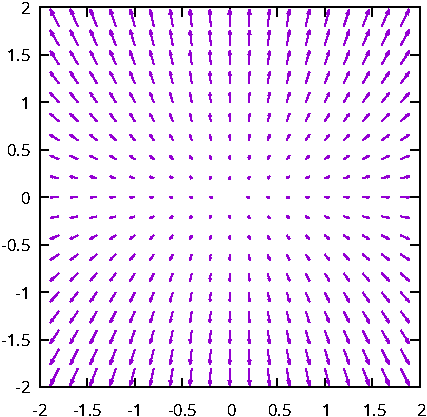
\includegraphics[width=.32\textwidth]{gnuplot/linear-pp-crop.pdf}
    \hfill
    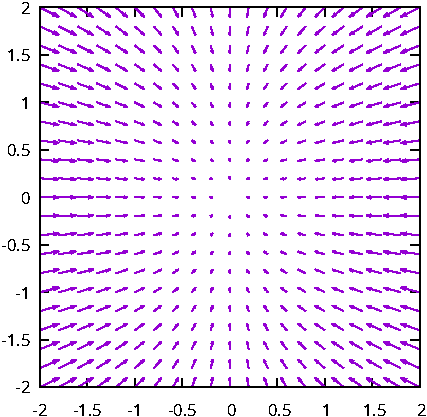
\includegraphics[width=.32\textwidth]{gnuplot/linear-mm-crop.pdf}
    \hfill
    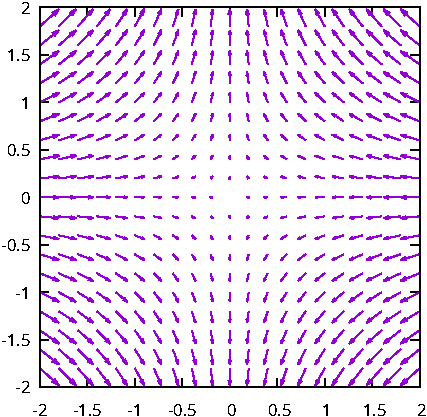
\includegraphics[width=.32\textwidth]{gnuplot/linear-pm-crop.pdf}
  \end{center}
\end{frame}

\begin{frame}
  \begin{exampleblock}{Diskussion}
    Reelle Matrizen können komplexe Eigenwerte haben. Offensichtlich
    wollen wir aber keine komplexwertigen Lösungen unserer AWA.
  \end{exampleblock}
\end{frame}

\begin{frame}{Komplexe Eigenwerte}
  \begin{block}{Satz}
    Hat eine reelle Matrix komplexe Eigenwerte, so treten sie als
    komplex konjugierte Paare mit ebensolchen Paaren von Eigenvektoren
    auf.
  \end{block}
  \pause
  Sei nun $r\pm i\phi$ ein solches Paar mit den Eigenvektoren $u\pm iv$
  \begin{align*}
    A (u\pm iv) &= {r+i\phi} (u\pm iv),\\
    e^A (u\pm iv) &= e^{r+i\phi} (u\pm iv) = e^r (\cos\phi \pm i \sin\phi)(u\pm iv).
  \end{align*}

  \vspace*{4cm}
\end{frame}

\begin{frame}
  \begin{block}{Reelle Lösungen}
    Hat die Matrix $A$ ein komplexes Eigenwertpaar
    $\lambda_{1/2} = r\pm i\phi$ mit zugehörigen Eigenvektoren
    $u\pm iv$, so ersetzen wir in der Transformationsmatrix die
    Eigenvektoren durch $u$ und $v$ und erhalten für $e^A$ eine
    quasi-Diagonalmatrix mit Block
    \begin{gather*}
      e^r
      \begin{pmatrix}
        \cos\phi & \sin\phi\\
        -\sin\phi & \cos \phi
      \end{pmatrix}
    \end{gather*}
  \end{block}
\end{frame}

\begin{frame}{Beispiele}
  \begin{center}
    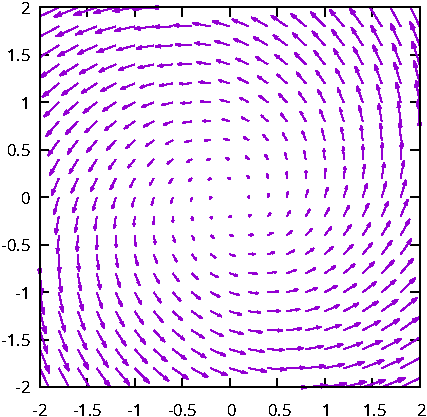
\includegraphics[width=.32\textwidth]{gnuplot/linear-cp-crop.pdf}
    \hfill
    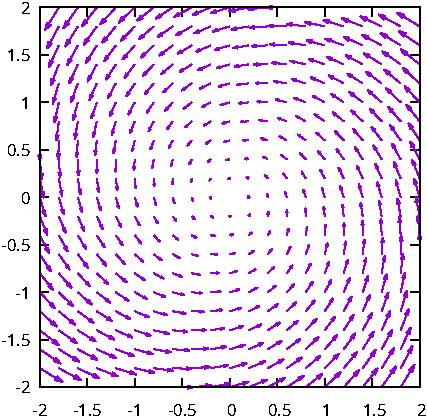
\includegraphics[width=.32\textwidth]{gnuplot/linear-cm-crop.pdf}
    \hfill
    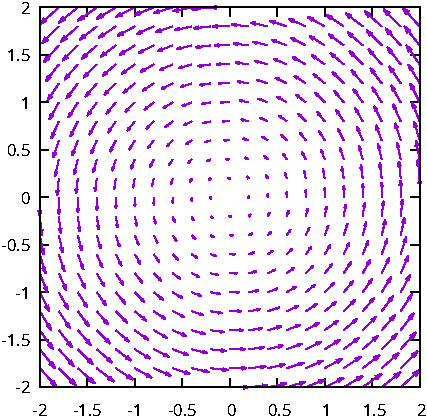
\includegraphics[width=.32\textwidth]{gnuplot/linear-c0-crop.pdf}
  \end{center}  
\end{frame}

%%%%%%%%%%%%%%%%%%%%%%%%%%%%%%%%%%%%%%%%%%%%%%%%%%%%%%%%%%%%%%%%%%%%%%
%%%%%%%%%%%%%%%%%%%%%%%%%%%%%%%%%%%%%%%%%%%%%%%%%%%%%%%%%%%%%%%%%%%%%%
\subsection{Berechnung von Lösungen anderer Gleichungen}

%%%%%%%%%%%%%%%%%%%%%%%%%%%%%%%%%%%%%%%%%%%%%%%%%%%%%%%%%%%%%%%%%%%%%%
%%%%%%%%%%%%%%%%%%%%%%%%%%%%%%%%%%%%%%%%%%%%%%%%%%%%%%%%%%%%%%%%%%%%%%
\subsection{Numerische Verfahren}



%%%%%%%%%%%%%%%%%%%%%%%%%%%%%%%%%%%%%%%%%%%%%%%%%%%%%%%%%%%%%%%%%%%%%%
%%%%%%%%%%%%%%%%%%%%%%%%%%%%%%%%%%%%%%%%%%%%%%%%%%%%%%%%%%%%%%%%%%%%%%
\begin{Abschluss}
\item Unter Annahme der Kontinuumshypothese können wir
  Wachtumsprozesse durch Differentialgleichungen
  beschreiben.
\item Populationsdynamik mehrerer Spezies führt zu Systemen von DGln.
\item Diese DGLn. haben unendlich viele Lösungen, was uns eigentlich interessiert, ist die Lösung einer Anfangswertaufgabe (AWA)
\item Das Ergebnis der eigentlichen Modellierung war die
  Volterrasche Integralgleichung
\end{Abschluss}


\begin{frame}{Zusammenfassung Analyse}
  \begin{enumerate}
  \item Qualitative Diskussion zum Verständnis der Modelle
    \begin{itemize}
    \item Richtungsfelder
    \item Phasenraumdiagramme
    \end{itemize}
  \item Verhalten für große Zeiten
    \begin{itemize}
    \item Fixpunkte
    \end{itemize}
  \item Wir haben die allgemeine Lösung der DGl. geraten und an den
    Anfangswert angeglichen
  \end{enumerate}
\end{frame}



%%%%%%%%%%%%%%%%%%%%%%%%%%%%%%%%%%%%%%%%%%%%%%%%%%%%%%%%%%%%%%%%%%%%%%
%%%%%%%%%%%%%%%%%%%%%%%%%%%%%%%%%%%%%%%%%%%%%%%%%%%%%%%%%%%%%%%%%%%%%%
%%%%%%%%%%%%%%%%%%%%%%%%%%%%%%%%%%%%%%%%%%%%%%%%%%%%%%%%%%%%%%%%%%%%%%
%%%%%%%%%%%%%%%%%%%%%%%%%%%%%%%%%%%%%%%%%%%%%%%%%%%%%%%%%%%%%%%%%%%%%%
%%%%%%%%%%%%%%%%%%%%%%%%%%%%%%%%%%%%%%%%%%%%%%%%%%%%%%%%%%%%%%%%%%%%%%


\begin{frame}
  \begin{block}{Homogene Differentialgleichungen}
    Eine Differentialgleichung ist homogen, wenn es keinen Summanden
    gibt, der die Lösungsfunktion nicht enthält. Einen solchen
    Summanden nennt man dann die Inhomogenität.
  \end{block}
  \begin{columns}
    \begin{column}[t]{.49\textwidth}
      \begin{block}{Homogen}
        \begin{gather*}
          x'+ \sin(t) x = 0
        \end{gather*}
      \end{block}
    \end{column}
    \begin{column}[t]{.49\textwidth}
      \begin{block}{Nicht homogen}
        \begin{gather*}
          x'+ \sin(t) x = 5
        \end{gather*}
      \end{block}
    \end{column}
  \end{columns}
  \only<1>{
  \begin{Denkpause}
    Welche Prozesse führen zu homogenen DGln., welche zu nicht homogenen?
  \end{Denkpause}}
\begin{itemize}
\item Homogene Gleichungen haben keine externen Quellen
\item Die null ist Lösung einer homogenen Gleichung
\end{itemize}
\end{frame}

%\mode*
\section{Auswirkungen von Eingabe- und Rechenfehlern}

Definition einer Rechenaufgabe

Fehlerquellen am Beispiel Lösung linearer Gleichungssysteme (geometrisch, Wdh. 1. Semester)

relative und absolute Fehler

Konditionierung/Stabilität von Lösungen

Konditionierung der Lösung eines LGS

Fehlerfortpflanzung additiver und multiplikativer Fehler (Vorlesung 3.3).

\mode<all>


%\section{Wahrscheinlichkeitstheorie}

\begin{frame}{Wahrscheinlichkeitstheorie vs. Statistik}
    \begin{itemize}
        \item Die \textbf{Wahrscheinlichkeitstheorie} versucht, die Ungewissheit zu \textbf{modellieren}. Es können also Vorhersagen gemacht werden (z.B. Umfragen vor einer Wahl).
        \item Die \textbf{beschreibende} (deskriptive) \textbf{Statistik} versucht, die Beobachtungen zu \textbf{beschreiben}. Es können keine Vorhersagen gemacht werden. 
        (Bsp.: Kommentare zum Ausgang einer Wahl, wie hat eine Personengruppe gewählt, etc...)
    \end{itemize}
\end{frame}

%%%%%%%%%%%%%%%%%%%%%%%%%%%%%%%%%%%%%%%%%%%%%%%%%%%%%%%%%%%%
%%%%%%%%%%%%%%%%%%%%%%%%%%%%%%%%%%%%%%%%%%%%%%%%%%%%%%%%%%%%
\subsection{Ereignisse und Wahrscheinlichkeiten}

\begin{frame}{Einführung am Beispiel: Sechsseitiger Würfel}
  \begin{itemize}
  \item \textbf{Zufallsexperiment}: der Würfel wird geworfen
  \item \textbf{Ergebnis} ist Element des Ergebnisraums:
    \begin{gather*}
      \Omega=\left\{\dice1,\dice2,\dice3,\dice4,\dice5,\dice6\right\}
    \end{gather*}
  \item \textbf{Ereignis} ist Teilmenge des Ergebnisraums $\Omega$
    \begin{itemize}
    \item $A = \left\{\dice1\right\}=$ \glqq eine 1 würfeln\grqq 
    \item $B = \left\{\dice2,\dice3\right\}=$\glqq eine 2 oder eine 3 würfeln\grqq 
    \item $C = \left\{\dice2,\dice4,\dice6\right\}=$\grqq eine gerade Zahl würfeln\grqq
    \end{itemize} 
  \item Ereignisse mit nur einem Element nennt man auch Elementarereignis
    \begin{itemize}
    \item Elementarereignis entspricht Ergebnis
    \end{itemize}
  \end{itemize}
\end{frame}

\begin{frame}{Die Menge der Ereignisse}
  \begin{itemize}
  \item \textbf{Potenzmenge} von $\Omega$: alle möglichen Teilmengen
    \begin{itemize}
    \item Achtung: $\{X,Y\} = \{Y,X\}$
    \end{itemize}
    \begin{multline*}
      \ereignisraum = \Bigl\{\emptyset
      ,\left\{\dice1\right\}
      ,\left\{\dice2\right\}
      ,\left\{\dice3\right\}
      ,\left\{\dice4\right\}
      ,\left\{\dice5\right\}
      ,\left\{\dice6\right\}
      ,\left\{\dice1,\dice2\right\}
      ,\dots
      ,\left\{\dice1,\dice6\right\}
      ,\\\left\{\dice2,\dice3\right\}      
      ,\left\{\dice3,\dice4\right\}
      ,\dots
      ,\left\{\dice3,\dice6\right\}      
      ,\dots
      ,\left\{\dice5,\dice6\right\}
      ,\\\left\{\dice1,\dice2,\dice3\right\}      
      ,\dots
      ,\left\{\dice1,\dice3,\dice4\right\}      
      ,\dots
      ,\left\{\dice4,\dice5,\dice6\right\} 
      ,\\\left\{\dice1,\dice2,\dice3,\dice4\right\}
      ,\left\{\dice3,\dice4,\dice5,\dice6\right\} 
      ,\\\left\{\dice1,\dice2,\dice3,\dice4,\dice5\right\}
      ,\left\{\dice2,\dice3,\dice4,\dice5,\dice6\right\} 
      ,\Omega\Bigr\}
    \end{multline*}
    \item Insgesamt $2^6$ Elemente
  \end{itemize}
\end{frame}

\begin{frame}{Wahrscheinlichkeiten}
  Die Wahrscheinlichkeit $P$ auf dem Ereignisraum $\ereignisraum$ ordnet
  jedem Element $A\in \ereignisraum$ eine Zahl zu. Es gilt:
  \begin{itemize}
  \item $0 \le P(A) \le 1$
  \item $P(\Omega) = 1$
  \item $P(A\cup B) = P(A)+P(B)$ falls $A\cap B=\emptyset$
    \begin{itemize}
    \item $P(A\cup B)$, Wahrscheinlichkeit, dass $A$ oder $B$ eintritt
    \end{itemize}
    \pause
  \item Dies gilt auch für beliebige Vereinigungen, wenn die Mengen
    sich paarweise nicht schneiden
    \begin{gather*}
      P\left(\bigcup_i A_i\right) = \sum_i P(A_i)
    \end{gather*}
  \end{itemize}
\end{frame}

\begin{frame}{Beispiel: sechsseitiger Würfel}
  \begin{itemize}
  \item Der Würfel ist nicht gezinkt:
    \begin{gather*}
      P(\{\dice1\}) = P(\{\dice2\}) = P(\{\dice3\}) = P(\{\dice4\}) = P(\{\dice5\}) = P(\{\dice6\}) = \frac16
    \end{gather*}
  \item Für Teilmengen $A$ mit $m$ Elementen gilt $P(A)=m/6$
    \begin{gather*}
      P(\{\dice1,\dice4\}) = \frac26=\frac13,
      \qquad
      P(\{\dice1,\dice4,\dice5\}) = \frac36=\frac12
    \end{gather*}
  \end{itemize}
\end{frame}

\begin{frame}{Beispiel: zwei sechsseitige Würfel}
  \begin{itemize}
  \item Zufallsexperiment: zwei identische Würfel werden gleichzeitig geworfen.
    \begin{gather*}
      \Omega = \left\{
        \begin{bmatrix}
          \dice1\\\dice1
        \end{bmatrix}
        ,
        \begin{bmatrix}
          \dice1\\\dice2
        \end{bmatrix}
        ,\dots,
        \begin{bmatrix}
          \dice1\\\dice6
        \end{bmatrix}
        ,
        \begin{bmatrix}
          \dice2\\\dice1
        \end{bmatrix}
        ,\dots,
        \begin{bmatrix}
          \dice2\\\dice6
        \end{bmatrix}
        ,
        \begin{bmatrix}
          \dice3\\\dice1
        \end{bmatrix}
        ,\dots,
        \begin{bmatrix}
          \dice6\\\dice6
        \end{bmatrix}
        \right\}
      \end{gather*}
    \item<3-> Bei identischen Würfeln kann die Reihenfolge nicht
      beobachtet werden, also nicht die Ereignisse
      \begin{gather*}
        \left\{\begin{bmatrix}
          \dice1\\\dice2
        \end{bmatrix}\right\}
        \quad\text{und}\quad
        \left\{\begin{bmatrix}
          \dice2\\\dice1
        \end{bmatrix}\right\}
      \quad\text{aber die Vereinigung}\quad
        \left\{\begin{bmatrix}
          \dice1\\\dice2
        \end{bmatrix}
        ,\begin{bmatrix}
          \dice2\\\dice1
        \end{bmatrix}\right\}
    \end{gather*}
  \item<3-> Wir definieren also den Ereignisraum
    \begin{gather*}
      \hspace*{-1em}
      \ereignisraum = \left\{\!
        \left\{\!
          \begin{bmatrix}
            \dice1\\\dice1
          \end{bmatrix}
          \!\right\}\!,\!
        \left\{\!
          \begin{bmatrix}
            \dice1\\\dice2
          \end{bmatrix}
          \!\!,\!\!
          \begin{bmatrix}
            \dice2\\\dice1
          \end{bmatrix}
          \!\right\}\!,\!
        \left\{\!
          \begin{bmatrix}
            \dice1\\\dice3
          \end{bmatrix}
          \!\!,\!\!
          \begin{bmatrix}
            \dice3\\\dice1
          \end{bmatrix}
          \!\right\}
        ,\dots,
        \left\{\!
          \begin{bmatrix}
            \dice2\\\dice2
          \end{bmatrix}
          \!\right\}
        \!,\!
        \left\{
          \begin{bmatrix}
            \dice2\\\dice3
          \end{bmatrix}
          \!\!,\!\!
          \begin{bmatrix}
            \dice3\\\dice2
          \end{bmatrix}
          \!\right\},\dots        
        \!\right\}
    \end{gather*}
    
  \end{itemize}
  \only<2>{
    \begin{Denkpause}
      Sind alle Ergebnisse beobachtbar?
    \end{Denkpause}
  }
\end{frame}

\begin{frame}{Ereignisraum und $\sigma$-Algebra}
  Ist $\ereignisraum$ nicht die Potenzmenge von $\Omega$, sondern eine
  andere Menge von Teilmengen, dann fordern wir folgende
  Eigenschaften:
  \begin{enumerate}
  \item $\Omega\in\ereignisraum$
  \item Falls $A\in\ereignisraum$, dann ist das Komplement $A^c\in\ereignisraum$.
  \item Falls $A_i\in\ereignisraum$ für $i=1,2,\dots$, dann ist
    \begin{gather*}
      \bigcup_{i} A_i\in\ereignisraum
    \end{gather*}
  \end{enumerate}
  Eine Menge von Teilmengen von $\Omega$ mit diesen Eigenschaften
  nennt man eine $\sigma$-Algebra über $\Omega$.

  \pause

  Auf einer $\sigma$-Algebra $\ereignisraum$ kann eine
  Wahrscheinlichkeit $P$ definiert werden.
\end{frame}

\begin{frame}{Beispiel: Konzentrationen}
  \begin{itemize}
  \item Ergebnis eines Zufallsexperiments: pH-Wert
    \begin{itemize}
    \item $\Omega = (0,14]$ (halboffen aus praktischen Gründen)
    \item Die Potenzmenge der reellen Zahlen ist ein mathematisches Monster
      \begin{itemize}
      \item Ungeeignet für die Definition der Wahrscheinlichkeit
      \end{itemize}
    \end{itemize}
    \pause
  \item Sie haben ein billiges pH-Meter, das nur ganzzahlig ausgibt
    \begin{itemize}
    \item Die \glqq{}Atome\grqq{} der passenden $\sigma$-Algebra sind die Mengen
      \begin{gather*}
        \bigl\{ x\in(0,14]\big| i-1<x\le i\bigr\},\quad i=1,\dots,14
      \end{gather*}
    \item Alle weiteren Teilmengen, inklusive $\Omega$ entstehen
      durch Vereinigungen
    \item Die $\sigma$-Algebra bildet mögliches Wissen über die Zufallsergebnisse ab
    \end{itemize}
    \pause
  \item Die sogenannte Borelsche $\sigma$-Algebra bildet den
    Informationsgehalt der reellen Zahlen ab
  \end{itemize}
\end{frame}

\begin{Aufgabe}
  Was wäre die $\sigma$-Algebra $\ereignisraum $ bei einem doppelten Münzwurf, falls
  \begin{enumerate}
  \item zwei Münzen gleichzeitig geworfen werden?
  \item zwei Münzen nacheiander geworfen werden?
  \end{enumerate}
\end{Aufgabe}

\begin{frame}{Überlappende Ereignisse}
  \begin{gather*}
    A\cap B \neq \emptyset
  \end{gather*}
  \begin{itemize}
  \item Die beiden Ereignisse können gleichzeitig eintreten
  \item  Beispiel Würfel:
    \begin{align*}
      A&=\left\{\dice2,\dice4,\dice6\right\},
      \\B&=\left\{\dice1,\dice2,\dice3\right\},
      \\A\cap B&= \left\{\dice2\right\} \\
      P(A\cap B) &= \frac{1}{6}
    \end{align*}
  \end{itemize}
\end{frame}

\begin{frame}{Siebformel für überlappende Ereignisse}
    \begin{itemize}
        \item Für 2 Ereignisse $A$ und $B$ gilt im Allgemeinen:
        \begin{gather*}
            P(A\cup B) = P(A) +P(B)-P(A\cap B)    
        \end{gather*}
        \item  Beispiel Würfel:
        \begin{gather*}
          A=\left\{\dice2,\dice4,\dice6\right\},
          \ B=\left\{\dice3,\dice4,\dice5,\dice6\right\},
          \ A\cap B= \left\{\dice4,\dice6\right\} \\
            \Rightarrow P(A\cap B) = \frac{2}{6}
        \end{gather*}
        \item also gilt 
        \begin{gather*}
            P(A\cup B)= \frac{3}{6} + \frac{4}{6} - \frac{2}{6} = \frac{5}{6}
        \end{gather*}
    \end{itemize}
\end{frame}

\begin{frame}{Siebformel für überlappende Ereignisse}
  Für $n$ Ereignisse gilt allgemein:
  \begin{multline*}
    P\left(\bigcup_iA_i\right)
    =\sum_iP(A_i)-\sum_{i<j}P(A_i\cap A_j) \\
    + \sum_{i<j<k}P(A_i\cap A_j \cap A_k) - \dots
  \end{multline*}

  \begin{itemize}
  \item Zunächst subtrahiert man von der Summe alle Schnitte, da diese
    doppelt gezählt wurden
  \item Dabei hat man aber die Schnitte dreier Ereignisse zweimal
    subtrahiert, deswegen addiert man sie wieder
  \item Nun hat man denselben Fehler mit Schnitten von vier Ereignissen gemacht
  \item ...
  \end{itemize}
\end{frame}

\begin{frame}{Eigenschaften der Wahrscheinlichkeit}
  \begin{itemize}
  \item Komplement $P(A^c) = 1-P(A)$, Wahrscheinlichkeit, dass $A$ nicht eintritt
  \item Unmögliches Ereignis $P(\emptyset)=0$
  \item wenn $A\subseteq B \Rightarrow P(A) \leq P(B)$
  \item $P(A\cup B)\leq P(A)+P(B)$
  \end{itemize}
\end{frame}

\begin{frame}{Bedingte Wahrscheinlichkeit}
    \begin{itemize}
        \item \textbf{Bedingte Wahrscheinlichkeit} bezeichnet die Wahrscheinlichkeit eines Ereignisses $A$ unter dem Wissen, dass Ereignis $B$ bereits eingetreten ist (geschrieben: $P(A|B)$
        \item Sie ist definiert als:
        \begin{gather*}
            P(A|B) = \frac{P(A\cap B)}{P(B)}
        \end{gather*}
        \item \textit{"Wie oft sind $A$ und $B$ aufgetreten, gemessen an der Häufigkeit von $B$ allein?}
    \end{itemize} 
    \includegraphics[width=0.8\textwidth]{fig/bedingte_Wahrscheinlichkeit.tikz}
\end{frame}

\begin{frame}{Vorsorgetests}
  \begin{itemize}
  \item Sie testen auf eine seltene, zunächst syptomlose Erkrankung
    \begin{itemize}
    \item Prävalenz 0.1\%
    \end{itemize}
  \item Die gesamte Bevölkerung wird getestet
    \begin{itemize}
    \item Sensitivität 99\%
    \item Spezifität 99\%
    \end{itemize}
  \item<3-> Bei Bevölkerung 1M sind 1000 erkrankt
    \begin{itemize}
    \item Positive Tests $1000\cdot 99\%=990$
    \end{itemize}
  \item<4-> Es sind $1M-1000= 999000$ gesund
    \begin{itemize}
    \item Positive Tests $999000\cdot 1\% = 9990$
    \end{itemize}
  \item<5-> Seien $T$ und $K$ die Ereignisse pos. Test und krank
    \begin{gather*}
      P(T) = \frac{10980}{1M},\quad
      P(T\cap K) = \frac{990}{1M},\quad
      P(K|T) = \frac{990}{10980} \approx 9\%
    \end{gather*}
    \item<5-> Die bedingte Wahrscheinlichkeit hängt von der Prävalenz ab
  \end{itemize}
  \begin{onlyenv}<2>
    \begin{Denkpause}
      Wie hoch ist bei einem positiven Testergebnis die
      Wahrscheinlichkeit, erkrankt zu sein?
    \end{Denkpause}
  \end{onlyenv}
\end{frame}

%%%%%%%%%%%%%%%%%%%%%%%%%%%%%%%%%%%%%%%%%%%%%%%%%%%%%
\begin{frame}
    \frametitle{Satz der totalen Wahrscheinlichkeit}
\label{totprob}
    \begin{center}
        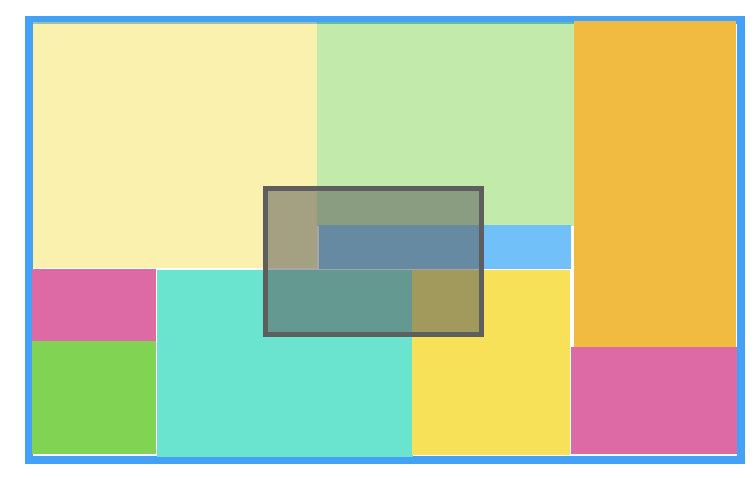
\includegraphics[width=.6\textwidth]{fig/prob03.png}
    \end{center}
    \begin{itemize}
    \item $A_i$ disjunkte Ereignisse, sodass $\cup_i A_i = \Omega$
    \item Dann gilt für ein Ereignis $B$:
      \begin{gather*}
        P(B) = \sum_i P(A_i)\frac{P(B\cap A_i)}{P(A_i)}
        \visible<2>{= \sum_i P(A_i)\,P(B|A_i)}
      \end{gather*}
    \end{itemize}
\end{frame}


%%%%%%%%%%%%%%%%%%%%%%%%%%%%%%%%%%%%%%%%%%%%%%%%%%%%%
\begin{frame}
    \frametitle{Bayes' Formel}

    \begin{itemize}
        \item Da $P(A\cap B) = P(B \cap A)$ können wir bei der Formel für die bedingte Wahrscheinlichkeit $A$ und $B$ vertauschen; daher gilt:
        $$
        P(A\cap B) = P(A|B)\,P(B) = P(B|A)\,P(A)
        $$  
        \item Daraus leiten wir die {\bf Bayessche Formel} her:
        $$
        P(A|B) = \frac{P(B|A)}{P(B)}\,P(A)
        $$
        \item $P(A)$ ist die {\em a priori} Wahrscheinlichkeit von $A$ (ohne vorheriges Wissen über andere Ereignisse!)
        \item $P(A|B)$ ist die {\em a posteriori} Wahrscheinlichkeit nach der Beobachtung von $B$
        \item Grundlage der Bayeschen Statistik
    \end{itemize}
\end{frame}

%%%%%%%%%%%%%%%%%%%%%%%%%%%%%%%%%%%%%%%%%%%%%%%%%%%%%%%%%%%%

\begin{frame}{Beispiel Vorsorgetest}
  \begin{itemize}
  \item Mit der Bayesschen Formel können wir die bedingte
    Wahrscheinlichkeit direkt ausrechnen:
    \begin{itemize}
    \item $P(K)$ Prävalenz
    \item $P(T|K)$ Sensitivität
    \item $1-P(T|K^c)$ Spezifität
    \end{itemize}
  \item Zu berechnen: $P(T)$
    \only<article>{unter Benutzung der totalen Wahrscheinlichkeit.}
    \begin{align*}
      P(T) &= P(T|K)P(K) + P(T|K^c)P(K^c) \\
      &= 0.99\times0.001 + 0.01\times 0.999 = 0.01098
    \end{align*}
  \item Einsetzen in Bayes' Formel ergibt
    \begin{align*}
      P(K|T) &= \frac{P(T|K)}{P(T)}P(K)\\
             &= \frac{0.99}{0.01098} \times  0.001 \approx 0.09016
    \end{align*}
  \end{itemize}
\end{frame}

%%%%%%%%%%%%%%%%%%%%%%%%%%%%%%%%%%%%%%%%%%%%%%%%%%%%%
\begin{frame}
  \frametitle{Bayes Formel und totale Wahrscheinlichkeit}

  Wir haben soeben folgende Eigenschaft benutzt, die sich aus der
  Kombination der Bayesschen Formel mit der totalen Wahrscheinlichkeit
  ergibt:
  \begin{itemize}
  \item $A_i$ disjunkte Ereignisse, sodass
    \begin{gather*}
      \bigcup_i A_i = \Omega
    \end{gather*}
  \item Dann gilt für ein Ereignis $B$:
    \begin{gather*}
      P(A_j|B) =  \frac{P(B|A_j)}{\sum_i P(B|A_i)P(A_i)}\,P(A_j)
    \end{gather*}
  \end{itemize}
\end{frame}

%%%%%%%%%%%%%%%%%%%%%%%%%%%%%%%%%%%%%%%%%%%%%%%%%%%%%
\begin{frame}
    \frametitle{Beispiel}

    \begin{itemize}
        \item Zwei Mitarbeiter einer Firma $M_1$, $M_2$ bearbeiten Anträge
        \item $M_1$ hat $P_1=40\%$ der Anträge bearbeitet, $M_2$ $P_2=60\%$
        \item $M_1$ hat eine Fehlerquote von 5\%, dh.\  $P(F|M_1)=0.05$
        \item $M_2$ hat eine Fehlerquote von 8\%, dh.\  $P(F|M_2)=0.08$
        \item Bei einem Antrag wurde eine fehlerhafte Bearbeitung festgestellt; was ist die Wahrscheinlichkeit, dass er von $M_1$ bearbeitet wurde?
        \item Lösung: wir suchen $P(M_1|F)$:
        \begin{eqnarray*}
        P(M_1|F) &=& \frac{P(F|M_1)}{P(F|M_1)P(M_1)+ P(F|M_2)P(M_2)}\,P(M_1) \\
        &=& \frac{0.05}{0.05\times 0.4 + 0.08\times 0.6}\times 0.4 = 29.4\%
        \end{eqnarray*}
    \end{itemize}
\end{frame}

%%%%%%%%%%%%%%%%%%%%%%%%%%%%%%%%%%%%%%%%%%%%%%%%%%%%%
\begin{frame}
    \frametitle{Unabhängige Ereignisse}

    \begin{itemize}
        \item Definition: zwei Ereignisse $A$ und $B$ sind {\bf unabhängig}, wenn gilt:
        $$
        P(A \cap B) = P(A)\cdot P(B)
        $$  
        \item Benutzt man die Bayes Formel folgt daraus: sind $A$ und $B$ unabhängig, dann gilt: $P(A|B) = P(A)$; das Wissen über $B$ verändert nicht die a posteriori Wahrscheinlichkeit von $A$
        \begin{itemize}
            \item Wahrscheinlichkeit, dass er regnet, gegeben, dass der Tag ein Montag ist: $P(Regen|Montag) = P(Regen)$
            \item Wahrscheinlichkeit, dass er regnet, gegeben, dass der Monat November ist: $P(Regen|November) \neq P(Regen)$ da Regen und November nicht unabhängig sind!
        \end{itemize}
    \end{itemize}
    

\end{frame}

%%%%%%%%%%%%%%%%%%%%%%%%%%%%%%%%%%%%%%%%%%%%%%%%%%%%%
\begin{frame}
  \frametitle{Unabhängige Ereignisse}
  
  \begin{itemize}
  \item Achtung: Unabhängigkeit und Disjunktheit sind nicht identisch!
  \item Disjunktheit von $A$ und $B$:
    \begin{gather*}
      P(A \cap B) =0
    \end{gather*}
  \item Unabhängigkeit von $A$ und $B$:
    \begin{gather*}
      P(A \cap B) =P(A)\,P(B)
    \end{gather*}
  \item \textbf{Vollständige} oder \textbf{gegenseitige} Unabhängigkeit bei mehreren Ereignissen $A_1,\ldots,A_k$: für jede Wahl von $k$ Ereignissen $A_{i_1},\ldots,A_{i_k}$ gilt:
    $$
    P(A_{i_1} \cap \ldots \cap A_{i_k}) = P(A_{i_1})\,P(A_{i_2})\ldots P(A_{i_k})
    $$
  \end{itemize}    
\end{frame}

%%%%%%%%%%%%%%%%%%%%%%%%%%%%%%%%%%%%%%%%%%%%%%%%%%%%%%%%%%%%
\begin{frame}{Beispiel: wiederholte Würfe eines Würfels}
  \begin{itemize}
  \item Ein sechsseitiger Würfel werde $5$ mal geworfen.
  \item In jedem Wurf ist die Wahrscheinlichkeit jeder Zahl 1/6
    \begin{itemize}
    \item ...unabhängig von allen vorherigen Würfen
    \end{itemize}
  \end{itemize}
  \begin{multline*}
    P\!\left(
      \begin{matrix}
        \dice6\\\dice6\\\dice6\\\dice6\\\dice6
      \end{matrix}
    \right)
    =
    P\!\left(
      \begin{matrix}
        \dice6\\ \\ \\ \\\phantom{\dice6}
      \end{matrix}
    \right)\times
    P\!\left(
      \begin{matrix}
        \\\dice6 \\ \\ \\\phantom{\dice6}
      \end{matrix}
    \right)\times
    P\!\left(
      \begin{matrix}
        \\ \\\dice6 \\ \\\phantom{\dice6}
      \end{matrix}
    \right)\times
    P\!\left(
      \begin{matrix}
        \\ \\ \\\dice6 \\\phantom{\dice6}
      \end{matrix}
    \right)\times
    P\!\left(
      \begin{matrix}
        \\ \\ \\ \\\dice6
      \end{matrix}
    \right)\\
    =\frac16\frac16\frac16\frac16\frac16 = \frac1{7776}
  \end{multline*}
\end{frame}


%%%%%%%%%%%%%%%%%%%%%%%%%%%%%%%%%%%%%%%%%%%%%%%%%%%%% 
\begin{frame}
  \frametitle{Abschlussfragen}
  
  \begin{enumerate}
  \item Was ist die Potenzmenge $\mathcal{S}$ beim Münzwurf (Kopf oder Zahl)?
  \item Müssen Sie Sensitivität oder Spezifität erhöhen, um den Test
    signifikant zu verbessern?
  \item Wieviele Anträge hätte $M_1$ bearbeiten müssen damit bei einem
    fehlerhaften Antrag eine 50/50 Chance besteht, dass er von $M_1$
    bearbeitet wurde?
  \end{enumerate}
\end{frame}
  


%%%%%%%%%%%%%%%%%%%%%%%%%%%%%%%%%%%%%%%%%%%%%%%%%%%%%
%%%%%%%%%%%%%%%%%%%%%%%%%%%%%%%%%%%%%%%%%%%%%%%%%%%%%
\subsection{Kombinatorik}
%%%%%%%%%%%%%%%%%%%%%%%%%%%%%%%%%%%%%%%%%%%%%%%%%%%%%

\begin{frame}{Zählen}
  \begin{itemize}
  \item Bei endlichen Ergebnismengen benötigt man die Anzahl aller
    Ergebnisse, um die Wahrscheinlichkeit zu berechnen
    \begin{gather*}
      P(A) = \frac{\#A}{\#\Omega}
    \end{gather*}
  \item Kombinatorik beschäftigt sich mit dem Zählen möglicher Ergebnisse
  \item Kombinatorik untersucht, wie viele verschiedene Anordnungen,
    Auswahlen oder Zuordnungen unter gegebenen Bedingungen möglich
    sind.
  \end{itemize}
\end{frame}

\begin{frame}{Permutationen}
  \begin{itemize}
  \item Permutationen von $n$ Objekten sind die möglichen Vertauschungen der Reihenfolge
  \item Ihre Anzahl ist
    \begin{gather*}
      n! = 1\cdot 2\cdot \ldots \cdot n      
    \end{gather*}
  \item Beispiel: $3!=6$
    \begin{gather*}
      (\dice1,\dice3,\dice5),(\dice1,\dice5,\dice3),\\
      (\dice3,\dice1,\dice5),(\dice3,\dice5,\dice1),\\
      (\dice5,\dice3,\dice1),(\dice1,\dice1,\dice3)\phantom{,}
    \end{gather*}
  \end{itemize}
\end{frame}



\begin{frame}
  \frametitle{Kombinationen}
  \begin{itemize}
  \item Auswahl von $k$ Objekten aus $n$
  \item Reihenfolge ist irrelevant
  \item Ihre Anzahl ist der Binomialkoeffizient
    \begin{gather*}
      \binom{n}{k} = \frac{n!}{k!(n-k)!}
    \end{gather*}
  \item Beispiel: Lotto 6 aus 49
    \begin{gather*}
      \frac{49!}{6!\,43!} = \frac{44\times 45\times \dots\times 49}{6!}
      = \frac{10068347520}{720} = 13983816
    \end{gather*}
  \end{itemize}
\end{frame}    

\begin{frame}
  \frametitle{Variationen}
  \begin{itemize}
  \item Auswahl von $k$ Objekten aus $n$
  \item Die Reihenfolge zählt
  \item Ihre Anzahl ist
    \begin{gather*}
      \binom{n}{k}k! = \frac{n!}{(n-k)!}
    \end{gather*}
  \item Beispiel: Alle Ketten von zwei der DNA-Basen Adenin, Cytosin, Guanin und Thymin
    \begin{gather*}
      A-C 
    \end{gather*}
  \end{itemize}

\end{frame}

\begin{frame}
  \frametitle{Variationen mit Wiederholungen}
  \begin{itemize}
  \item Auswahl von $k$ Objekten aus $n$
  \item Die Reihenfolge zählt
  \item Objekte dürfen mehrfach auftreten
  \item Ihre Anzahl ist
    \begin{gather*}
      n^k
    \end{gather*}
  \item Beispiel: Alle Ketten von zwei der DNA-Basen Adenin, Cytosin, Guanin und Thymin
    \begin{gather*}
      \begin{matrix}
        A-A& A-C& A-G& A-T\\
        C-A& C-C& C-G& C-T\\
        G-A& G-C& G-G& G-T\\
        T-A& T-C& T-G& T-T
      \end{matrix}
      \qquad 4^2=16
    \end{gather*}
  \end{itemize}
\end{frame}

\begin{frame}
  \frametitle{Kombinationen mit Wiederholungen}
  \begin{itemize}
  \item Auswahl von $k$ Objekten aus $n$
  \item Reihenfolge irrelevant
  \item Objekte dürfen mehrfach auftreten
  \item Ihre Anzahl ist
    \begin{gather*}
      \binom{n+k-1}{k}
    \end{gather*}
  \item Beispiel: eine Schachtel mit 2 Macaron aus den Sorten Cassis, Framboise und Myrtille
    \begin{gather*}
      \{C,C\}, \{C,F\},\{C,M\},\{F,F\},\{F,M\},\{M,M\}
      \qquad
      \binom{3+2-1}{2} = \binom{4}{2} = 6
    \end{gather*}
  \end{itemize}
\end{frame}

%%%%%%%%%%%%%%%%%%%%%%%%%%%%%%%%%%%%%%%%%%%%%%%%%%%%%%%%%%%%
\begin{Abschluss}
\item Wie viele DNA-Sequenzen der Länge 20 gibt es?
\item Wie viele verschiedene Reihenfolgen können fünf Gene haben?
\item Wie viele Möglichkeiten gibt es, drei Proben aus zehn auszuwählen?  
\item Was ist wahrscheinlicher:
  \begin{enumerate}
  \item bei 4 Würfen mit einen Würfel wird mindestens eine 6 geworfen;
  \item bei 24 Würfen mit 2 Würfeln wird mindestens eine Doppelsechs geworfen
  \end{enumerate}
\item Wieviele Möglichkeiten gibt es, eine Schachtel mit 3 Macarons
  der Sorten Cassis, Framboise, Myrtille und Pamplemousse zu füllen,
  wobei beliebig viele von allen, Myrtille aber maximal einmal, drin
  sein dürfen?
\end{Abschluss}


%%%%%%%%%%%%%%%%%%%%%%%%%%%%%%%%%%%%%%%%%%%%%%%%%%%%%%%%%%%%
%%%%%%%%%%%%%%%%%%%%%%%%%%%%%%%%%%%%%%%%%%%%%%%%%%%%%%%%%%%%

\subsection{Zufallsvariablen}
\begin{itemize}
\item Wir definieren jetzt die {\bf Wahrscheinlichkeit} $P_X$ der Zufallsvariablen $X$ 
  \begin{eqnarray*}
    &&P_X([a,b]) \equiv P(X \in [a,b]) ~~~\text{(stetige ZV)} \\ 
    &&P_X(k) \equiv P(X=k) ~~~\text{(diskrete ZV)}
  \end{eqnarray*}
\item Die Wahrscheinlichkeit $P_X$ ist also eine Abbildung
  $$
  P_X : \mathbb{R} \text{ oder } \mathbb{N} \longrightarrow [0,1]
  $$
\end{itemize}


%%%%%%%%%%%%%%%%%%%%%%%%%%%%%%%%%%%%%%%%%%%%%%%%%%%%%
\begin{frame}
    \frametitle{Zufallsvariablen und Wahrscheinlichkeit}

    \centerline{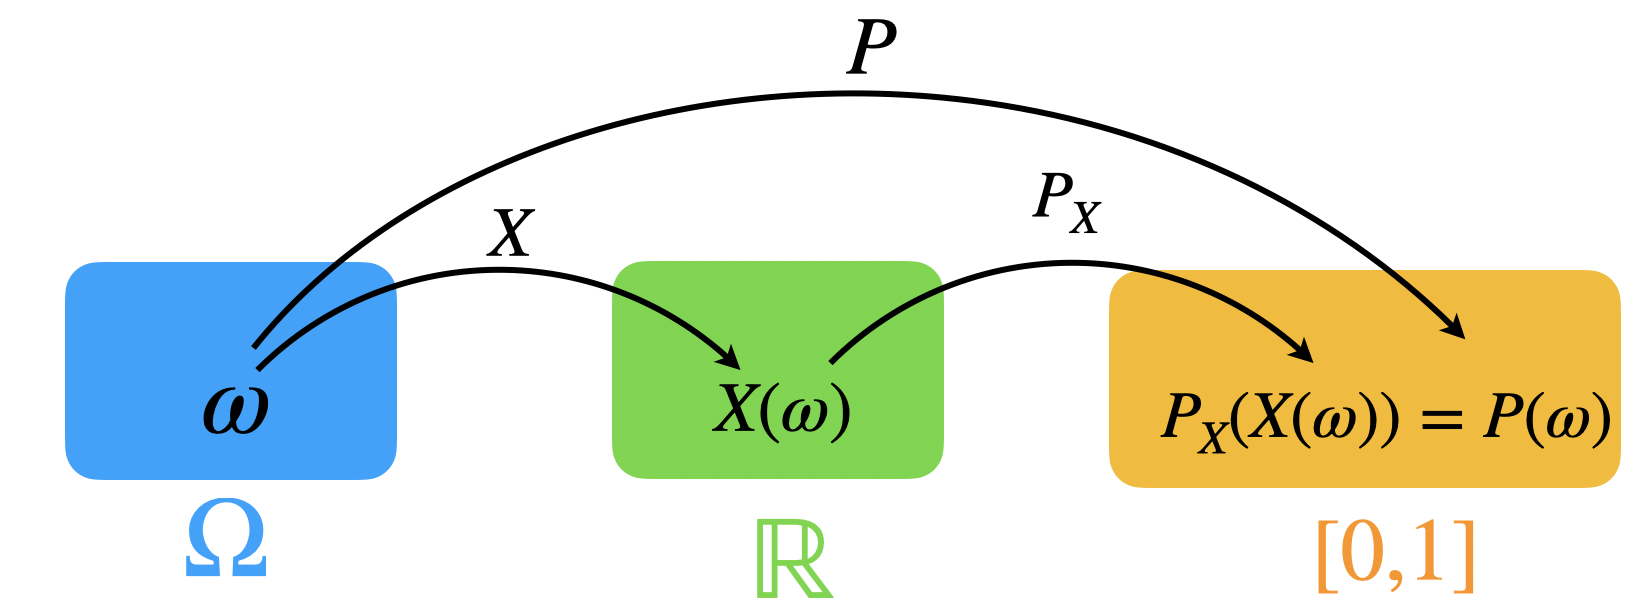
\includegraphics[width=.9\textwidth]{fig/prob09.png}}
\end{frame}

%%%%%%%%%%%%%%%%%%%%%%%%%%%%%%%%%%%%%%%%%%%%%%%%%%%%%
\begin{frame}
    \frametitle{Beispiel beim Münzspiel}


 \textbf{Ausgangssituation:}
\begin{itemize}
\item 3 Münzwürfe: $\Omega = {ZZZ, KZZ, ZKZ, ZZK, KKZ, KZK, ZKK, KKK}$
\item Jedes Ergebnis hat Wahrscheinlichkeit $(1/2)^3 = 1/8$
\end{itemize}
\vspace{0.5cm}
\textbf{Zufallsvariable} $X = $ "Anzahl der Zahlen"

\end{frame}

%%%%%%%%%%%%%%%%%%%%%%%%%%%%%%%%%%%%%%%%%%%%%%%%%%%%%
\begin{frame}
    \frametitle{Beispiel beim Münzspiel}

\textbf{Schritt 1:} Welche Werte kann $X$ annehmen?
\begin{itemize}
\item $X$ kann 0, 1, 2 oder 3 sein
\end{itemize}
\vspace{0.5cm}
\textbf{Schritt 2:} Für jeden Wert - welche Elementarereignisse führen dazu?

\vspace{0.5em}
\begin{tabular}{llll}
$X = 0$ & $\text{nur } KKK$ &$\Rightarrow$ & $P_X(0) = P(X = 0) = 1/8$\\
$X = 1$ & $KKZ, KZK, ZKK$ & $\Rightarrow$ & $P_X(1)=P(X = 1) = 3/8$\\
$X = 2$ & $KZZ, ZKZ, ZZK$ &$\Rightarrow$ & $P_X(2)=P(X = 2) = 3/8$\\
$X = 3$ & $\text{nur } ZZZ$ & $\Rightarrow$ & $P_X(3)=P(X = 3) = 1/8$
\end{tabular}
\end{frame}


%%%%%%%%%%%%%%%%%%%%%%%%%%%%%%%%%%%%%%%%%%%%%%%%%%%%%
\begin{frame}
    \frametitle{Diskrete Zufallsvariablen}

    \begin{itemize}
        \item Zufallsvariable: $X$ ; mögliche Realisationen: $x_i$
        \item Für diskrete Zufallsvariablen betrachten wir die {\bf Wahrscheinlichkeitsverteilung} 
        $$
        p_i = P(X = x_i)~~~~x_i = \text{abzählbare Realisationen}
        $$
        \item Es gilt
        $$
        \sum_i P(X=x_i) = 1
        $$  
        \item Die {\bf Verteilungsfunktion} ist hier:
        $$
        F_X(x) = P(X \le x) = \sum_{i: x_i \le x} P(X=x_i)
        $$
    \end{itemize}

\end{frame}

%%%%%%%%%%%%%%%%%%%%%%%%%%%%%%%%%%%%%%%%%%%%%%%%%%%%%
\begin{frame}
    \frametitle{Diskrete Zufallsvariablen}

    
    \begin{center}
        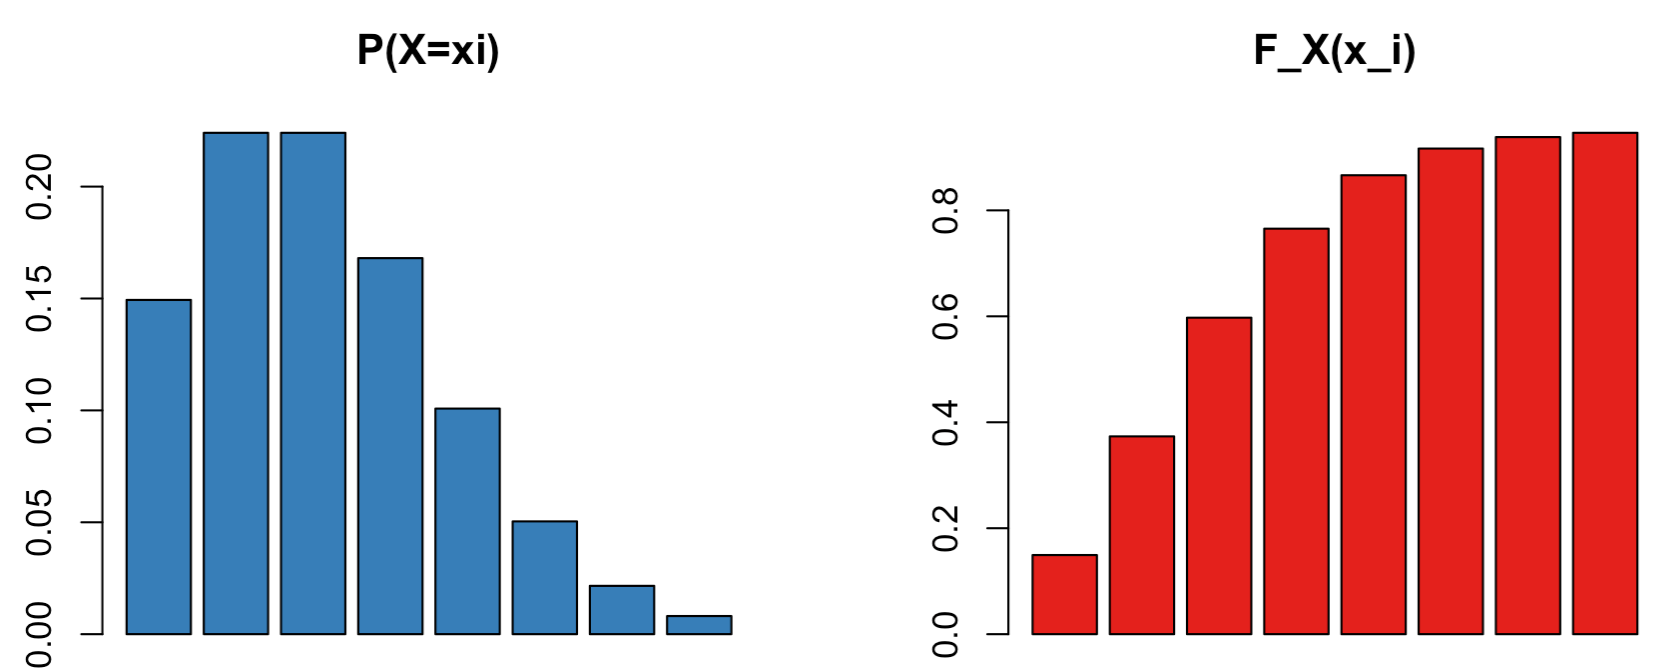
\includegraphics[width=.9\textwidth]{fig/prob04.png}
    \end{center}
    

\end{frame}




%%%%%%%%%%%%%%%%%%%%%%%%%%%%%%%%%%%%%%%%%%%%%%%%%%%%%
\begin{frame}
    \frametitle{Stetige Zufallsvariablen}

    \begin{itemize}
        \item Bei stetigen Zufallsvariablen ("Körpergröße; Regenmenge in einem Jahr; ...") gilt
        $
        P(X = x) =0
        $
        \item Anders ausgedrückt: Die Wahrscheinlichkeit, eine Person zu finden, die {\bf GENAU} 1,6 Meter groß ist ist Null \dots
        \item Wir betrachten stattdessen  die {\bf Wahrscheinlichkeitsdichte} $f(x): \mathbb{R} \to \mathbb{R}$ mit folgenden Eigenschaften:
    \end{itemize}
        \begin{enumerate}
            \item $P_X([a,b]) = P(X\in [a,b])= \int_{a}^{b} f(x)\,dx$ 
            \item $\int_{-\infty}^{\infty} f(x)\,dx = 1$
            \item $F_X(a) = P(X \le a) = \int_{-\infty}^{a} f(x)\,dx$
        \end{enumerate}
    

\end{frame}

%%%%%%%%%%%%%%%%%%%%%%%%%%%%%%%%%%%%%%%%%%%%%%%%%%%%%
\begin{frame}
    \frametitle{Stetige Zufallsvariablen}

    
    \begin{center}
        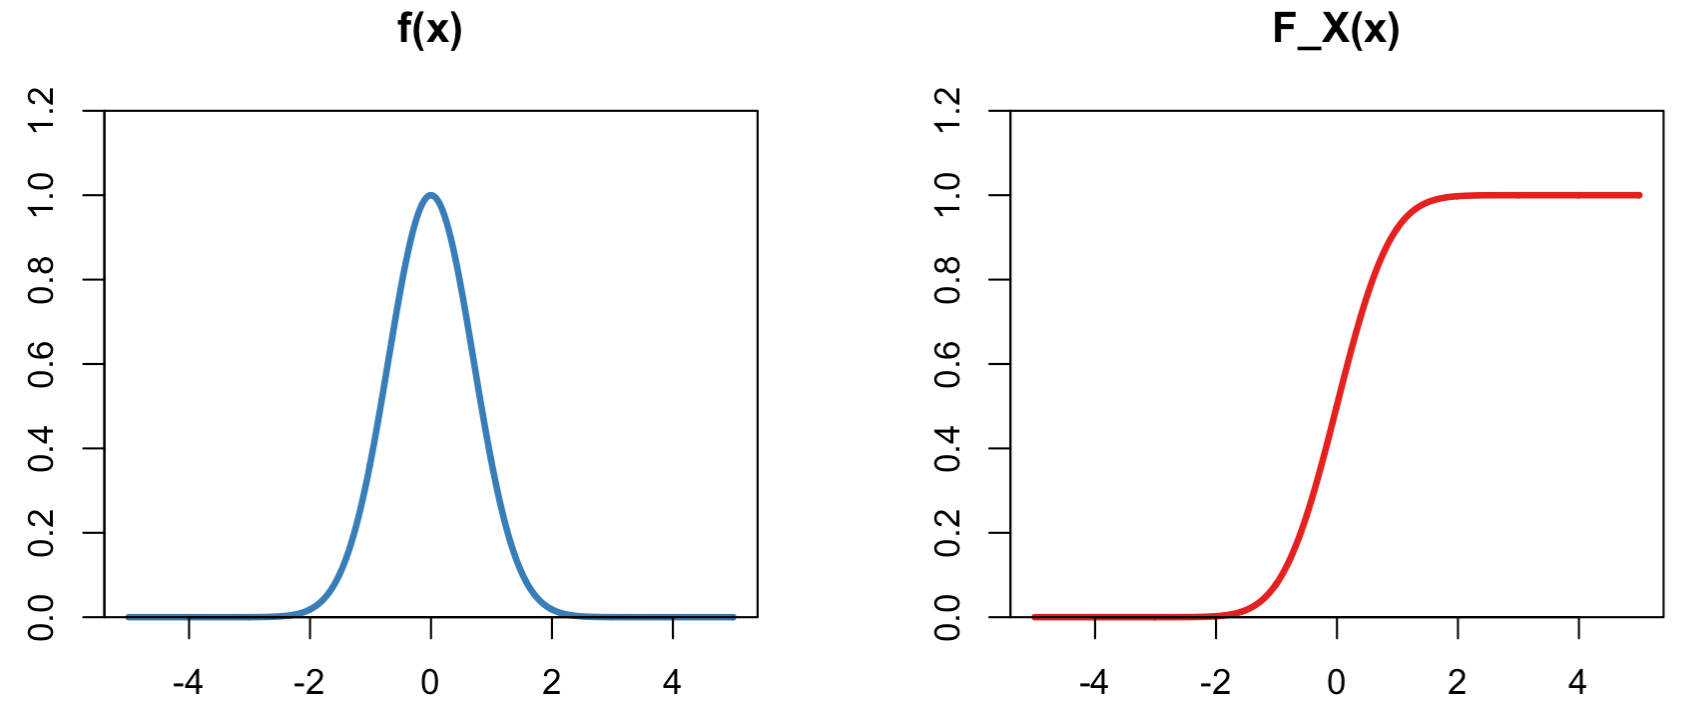
\includegraphics[width=.9\textwidth]{fig/prob05.png}
    \end{center}
    

\end{frame}




%%%%%%%%%%%%%%%%%%%%%%%%%%%%%%%%%%%%%%%%%%%%%%%%%%%%%
\begin{frame}
    \frametitle{Erwartungswert}

    Beispiel: Spiel mit gezinkter Münze:
    \begin{itemize}
        \item Zufallsvariable: $X$ = Gewinn bei einem Spiel: $x \in \{-1,+2\}$
        \item Kopf : $P(Kopf) = p$, Gewinn = +2 Euros
        \item Zahl : $P(Zahl) = 1-p$, Verlust  = -1 Euros
        \item Ab wann lohnt sich das Spiel?
        \item Erwartungswert: 
        \begin{eqnarray*}
        E(X) &=& (-1)\cdot P(X=-1) + (+2)\cdot P(X=+2)\\
        &=&  (-1)\cdot (1-p) + (+2)\cdot p = 3p-1
        \end{eqnarray*}
        \item Auf lange Sicht lohnt sich das Spiel, wenn $p>1/3$!
    \end{itemize}
    

\end{frame}


%%%%%%%%%%%%%%%%%%%%%%%%%%%%%%%%%%%%%%%%%%%%%%%%%%%%%
\begin{frame}
    \frametitle{Erwartungswert}

    \begin{itemize}
        \item Der Ewartungswert beschreibt den {\bf theoretischen durschnittlichen Wert} einer Zufallsvariablen.
           \item {\bf Erwartungswert bei diskreten Variablen:}:
        $$
        \mu \equiv E(X) = \sum_{i} x_i\,P(X=x_i)
        $$
        mit $x_i$ = mögliche Realisationen der Zufallsvariablen.
        \item {\bf Erwartungswert bei stetigen Variablen:}
        $$
        \mu \equiv E(X) = \int_{-\infty}^{+\infty} x\,f(x)\,dx
        $$
        mit $f(x)$ = Dichtefunktion der Zufallsvariablen.
 
    \end{itemize}
    

\end{frame}




%%%%%%%%%%%%%%%%%%%%%%%%%%%%%%%%%%%%%%%%%%%%%%%%%%%%%
\begin{frame}
    \frametitle{Varianz}

    \begin{itemize}
        \item Der Erwartungswert liefert den durschnittlichen Wert der Zufallsvariablen bei unendlich vielen Realisationen
        \item Aber wie stark streuen die Realisationen um den Erwartungswert?
        \item Diese Antwort liefert die {\bf Varianz}, die den Erwartungswert der quadratischen Abweichungen vom Erwartungswert gibt:
        $$
        \sigma^2 \equiv Var(X) = E((x-\mu)^2)
        $$
        \item Diskrete Zufallsvariable:
        $$
        Var(X) = \sum_i (x_i-\mu)^2\,P(X=x_i)
        $$
        \item Stetige Zufallsvariable:
        $$
        Var(X) = \int_{-\infty}^{+\infty} (x-\mu)^2\,f(x)\,dx
        $$
    \end{itemize}

\end{frame}


%%%%%%%%%%%%%%%%%%%%%%%%%%%%%%%%%%%%%%%%%%%%%%%%%%%%%
\begin{frame}
    \frametitle{Eigenschaften der Varianz}

    \begin{itemize}
        \item Es gilt:
        $$
        Var(X) = E(X^2) - \mu^2
        $$
        \item Invarianz bei Verschiebungen:
        $$
        Var(a+b\,X) = b^2\,Var(X)~~~~~a,b\in \mathbb{R}
        $$
        \item Sind $X_i$ paarweise {\bf unkorreliert} (d.h.\ es gilt $E(X_iX_j)= E(X_i)E(X_j)~~\forall i,j$), dann:
        $$
        Var(\sum_i X_i) = \sum_i Var(X_i)
        $$
    \end{itemize}

\end{frame}

%%%%%%%%%%%%%%%%%%%%%%%%%%%%%%%%%%%%%%%%%%%%%%%%%%%%%
\begin{frame}
    \frametitle{Unabhängigkeit von Zufallsvariablen}
\label{independent}

    {\bf Definition von identisch verteilten Zufallsvariablen:}\\

    \begin{itemize}
        \item 10 Personen Würfeln nacheinander; $X_i$ = gewürfelte Zahl der $i$-ten Person
        \item Es gilt $P(X_i=x) = P(X_j=x)$
        \item Die Zufallsvariablen $X_i$ und $X_j$ sind {\bf identisch verteilt}
        \item Daher auch $F_{X_i}(x) = F_{X_j}(x)$: die Verteilungsfunktionen sind identisch.
    \end{itemize}
    

\end{frame}

%%%%%%%%%%%%%%%%%%%%%%%%%%%%%%%%%%%%%%%%%%%%%%%%%%%%%
\begin{frame}
    \frametitle{Unabhängigkeit von Zufallsvariablen}

    {\bf Definition der Unabhängigkeit:}\\

    \begin{itemize}
    \item zwei Zufallsvariablen $X$ und $Y$ sind {\bf unabhängig voneinander}, wenn
        $$
        P(X \le x | Y \le y) = P(X\le x) 
        $$
        oder
        $$
        P(X \le x \cap  Y \le y) = P(X \le x)\cdot P(Y \le y)
        $$
        \item Schreibweise: wir schreiben $P(X \le x , Y \le y)$ für $P(X \le x \cap  Y \le y)$

        \item $X$ hat keinen Einfluss auf $Y$: beide Variablen sind {\bf unabhängig}
    \end{itemize}
 
    

\end{frame}



%%%%%%%%%%%%%%%%%%%%%%%%%%%%%%%%%%%%%%%%%%%%%%%%%%%%%
\begin{frame}
    \frametitle{Verallgemeinerung auf $n$ Zufallsvariablen}

    {\bf Definition:}\\
    Gegeben seien $n$ Zufallsvariablen $X_i$; falls gilt
    \begin{itemize}
        \item $F_{X_i}(x) = F_{X_j}(x)$
        \item $\forall~i_{1},i_{2},\ldots i_{k}:$ 
        $$
        P(X_{i_1}=x_{i_1},\ldots,X_{i_k}=x_{i_k}) = P(X_{i_1}=x_{i_1})\cdot \ldots \cdot P(X_{i_k}=x_{i_k})
        $$
    \end{itemize}
    dann heißen die Variablen {\bf identisch verteilt und unabhängig} {\em ("independent, identically distributed" = i.i.d.)}
\begin{itemize}
    \item Beispiel: Replikate bei einer Versuchreihe (z.B.\ Gewicht von 10 Mäusen nach knock-out des Gens {\em ApoE}) werden meistens als i.i.d.\ betrachtet: kein Einfluss aufeinander und identische Verteilung
\end{itemize}
    
\end{frame}


%%%%%%%%%%%%%%%%%%%%%%%%%%%%%%%%%%%%%%%%%%%%%%%%%%%%
\begin{frame}
    \frametitle{Abschlussfragen}

    \begin{enumerate}
        \item Ein Würfel wird zweimal geworfen. Sei $X$ die Zufallsvariable "Summe der beiden Würfe". Bestimmen Sie $P(X = 7)$.
        \item Bei einem fairen Würfel (Werte 1,2,3,4,5,6 mit jeweils Wahrscheinlichkeit $1/6$): Berechnen Sie Erwartungswert $E(X)$ und Varianz $Var(X)$.
        \item Wie könnte die Spielregel auf Folie \ref{independent} verändert werden, sodass die Variablen nicht mehr unabhängig voneinander sind?
        \item Gegeben sei das Münzwurf-Beispiel aus der Vorlesung (3 Münzwürfe, $X$ = Anzahl der Zahlen). Berechnen Sie die Verteilungsfunktion $F_X(2)$.
    \end{enumerate}
    
\end{frame}
\subsection{Verteilungen}
%%%%%%%%%%%%%%%%%%%%%%%%%%%%%%%%%%%%%%%%%%%%%%%%%%%%%
\begin{frame}
    \frametitle{Diskrete Verteilungen: 1. Bernouilli-Verteilung}

    \begin{itemize}
        \item Ein {\bf Bernouilli-Versuch} ist ein Versuch mit 2 möglichen Ausgängen (z.B.\ Münzwurf); diese Ausgänge können wir mit 0 und 1 darstellen
        $$
        P(X = 1) = \theta~~~~P(X = 0) = 1-\theta
        $$
        \item Es gilt
        $$
        E(X) = \theta ~~~~Var(X) =  \theta\,(1-\theta)
        $$
    \end{itemize}
\end{frame}

%%%%%%%%%%%%%%%%%%%%%%%%%%%%%%%%%%%%%%%%%%%%%%%%%%%%%
\begin{frame}
    \frametitle{Diskrete Verteilungen: 2. Binomial-Verteilung}

    \begin{itemize}
        \item Die Binomial-Verteilung beschreibt die Anzahl $k$ von positiven Ereignissen in einer Reihe von $n$ Bernouilli-Versuchen
        \item z.B.\ Anzahl von Zahl bei 10 Münzwürfen, \ldots
        \item Wahrscheinlichkeitsverteilung:
        $$
        P(X = k) = \binom{n}{k} \theta^k (1-\theta)^{n-k}
        $$
        \item Es gilt:
        $$
        E(X) = n\,\theta ~~~~Var(X) =  n\,\theta\,(1-\theta)
        $$
    \end{itemize}

\end{frame}

%%%%%%%%%%%%%%%%%%%%%%%%%%%%%%%%%%%%%%%%%%%%%%%%%%%%%
\begin{frame}
    \frametitle{Diskrete Verteilungen: 2. Binomial-Verteilung}


    Binomial-Verteilungen mit $n=20$:
    \begin{center}
        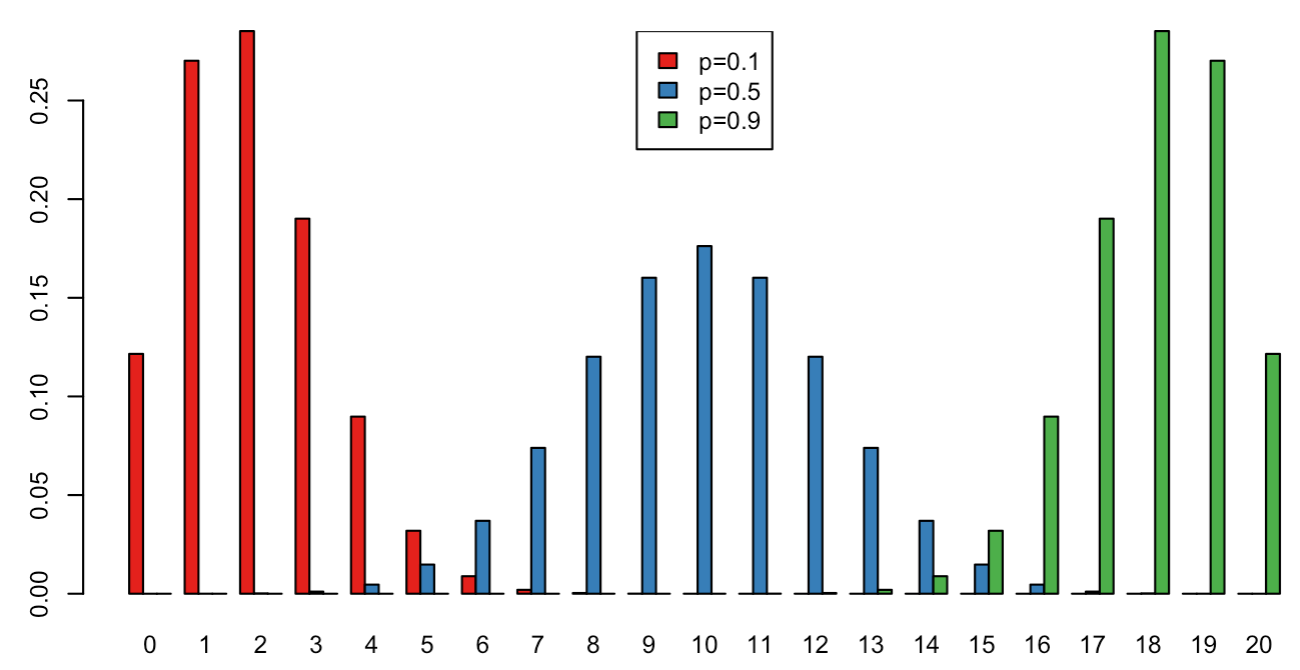
\includegraphics[width=\textwidth]{fig/prob07.png}
    \end{center}

\end{frame}

%%%%%%%%%%%%%%%%%%%%%%%%%%%%%%%%%%%%%%%%%%%%%%%%%%%%%
\begin{frame}
    \frametitle{2. Diskrete Verteilungen: Binomial-Verteilung}

    \begin{itemize}
        \item Beispiel: Polymerase hat eine Fehlerrate von 0.1\%; was ist die Wahrsheinlichkeit, dass eine Sequenz der Länge 1000 3 Fehler enthält?
        \item Wir definieren $X$ als "Anzahl der Fehler in der Sequenz der Länge 1000"
        $$
        P(X=3) = \binom{1000}{3}\,(0.001)^3\,(0.999)^{997} = 0.0612 \sim 6\%
        $$
    \end{itemize}

\end{frame}

%%%%%%%%%%%%%%%%%%%%%%%%%%%%%%%%%%%%%%%%%%%%%%%%%%%%%
\begin{frame}
    \frametitle{Diskrete Verteilungen: 2. Binomial-Verteilung}


    \begin{center}
        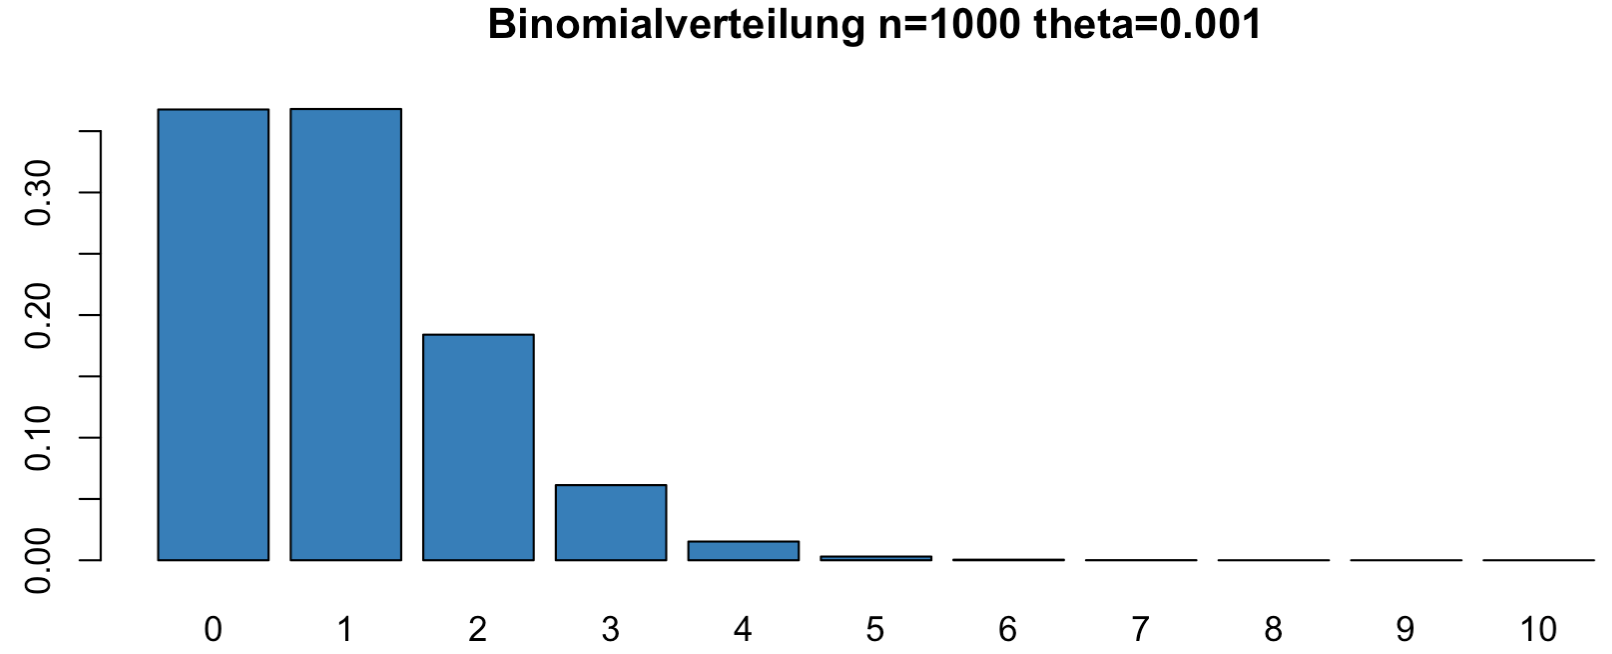
\includegraphics[width=0.8\textwidth]{fig/prob06.png}
    \end{center}

\end{frame}




%%%%%%%%%%%%%%%%%%%%%%%%%%%%%%%%%%%%%%%%%%%%%%%%%%%%%
\begin{frame}
    \frametitle{Diskrete Verteilungen: 3. Poisson-Verteilung}

\begin{itemize}
    \item Die Poisson-Verteilung beschreibt die Anzahl $k$ von erwarteten Ereignissen, wenn die {\bf Rate} $\lambda$ pro Messeinheit bekannt ist
    \item Zufallvariable $X$: Anzahl der beobachteten Ereignisse
    $$
    P(X = k) = \frac{\lambda^k}{k!}\,e^{-\lambda}
    $$
    \item Es gilt:
    $$
    E(X ) = \lambda ~~~~Var(X) = \lambda
    $$
    
\end{itemize}

\end{frame}

%%%%%%%%%%%%%%%%%%%%%%%%%%%%%%%%%%%%%%%%%%%%%%%%%%%%%
\begin{frame}
    \frametitle{Diskrete Verteilungen: 3. Poisson-Verteilung}

\begin{itemize}
\item Beispiel: Es gehen im Durschnitt $\lambda=10$ Anrufen pro Stunde in der Notfallzentrale ein; es wird ein Bonus bezahlt, falls in einer Schicht von 8 Stunden mehr als 100 Anrufen beantwortet werden. Was ist die Wahrscheinlichkeit, dass ein Bonus bezahlt wird?
\item Zufallvariable $X$ = Anzahl der Anrufe in 8 Stunden (Messeinheit = 1 Schicht = 8 Stunden)
\item Rate der Anrufe pro Schicht: $\lambda = 8*10 = 80$
\begin{eqnarray*}
P(X > 100) &=& 1- P(X \le 100) \\
&=& 1- \sum_{k=0}^{100} \frac{\lambda^k}{k!}\,e^{-\lambda} \\
&=& 0.01317 \sim 1.3 \%
\end{eqnarray*}
\end{itemize}
\end{frame}

%%%%%%%%%%%%%%%%%%%%%%%%%%%%%%%%%%%%%%%%%%%%%%%%%%%%%
\begin{frame}
    \frametitle{Stetige Verteilungen: 1.\ Exponential-Verteilung}

    \begin{itemize}
        \item Die Exponential-Verteilung beschreibt {\bf Wartezeiten}
        \item Zufallsvariable $X$ = Wartezeit, bis ein Ereignis vorkommt, wenn die Rate pro Einheit $\lambda$ ist
        \item Wahrscheinlichkeitsdichte:
        $$
f(x) = \lambda\,e^{-\lambda x} ~~~(x \ge 0)~~~~f(x) = 0 ~~~(x<0)
        $$
        \item Es gilt
        $$
        E(X) = \frac{1}{\lambda}~~~~Var(X) = \frac{1}{\lambda^2}
        $$
    \end{itemize}
    

\end{frame}

%%%%%%%%%%%%%%%%%%%%%%%%%%%%%%%%%%%%%%%%%%%%%%%%%%%%%
\begin{frame}
    \frametitle{Stetige Verteilungen: 1.\ Exponential-Verteilung}

    \begin{itemize}
        \item Beispiel: im Durschnitt wartet ein Kunde 20 Minuten in der Warteschleife einer Kundenhotline; was ist die Wahrscheinlichkeit, dass ich schon nach 5 Minuten drankomme?
        \item Zufallsvariable $X$= Wartezeit in Minuten; Rate der Antworten pro Minute: $\lambda = 1/20 = 0.05$
        \item Wir suchen $P(X\le 5)$:
        \begin{eqnarray*}
        P(X \le 5) &=& \int_{-\infty}^5 \lambda\,e^{-\lambda x}\,dx \\
        &=& \int_{0}^5 \lambda\,e^{-\lambda x}\,dx~~~~\text{da $f(x)=0$ für $x<0$} \\
        &=& [-e^{-\lambda x}]_0^5 \\
        &=& 1-e^{-0.05*5} = 0.22 \sim 22 \%
        \end{eqnarray*}
    \end{itemize}
    

\end{frame}

%%%%%%%%%%%%%%%%%%%%%%%%%%%%%%%%%%%%%%%%%%%%%%%%%%%%%
\begin{frame}
    \frametitle{Stetige Verteilungen: 1.\ Exponential-Verteilung}


    \begin{center}
        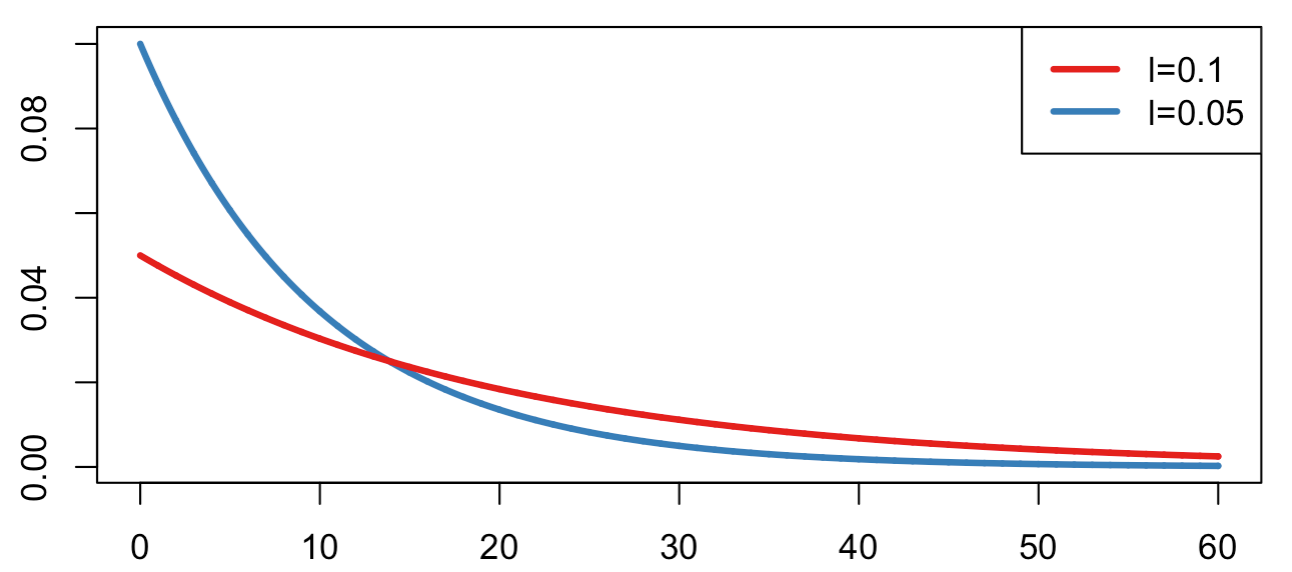
\includegraphics[width=0.8\textwidth]{fig/prob08.png}
    \end{center}

\end{frame}

%%%%%%%%%%%%%%%%%%%%%%%%%%%%%%%%%%%%%%%%%%%%%%%%%%%%%
\begin{frame}
    \frametitle{Stetige Verteilungen: 2.\ Normal-Verteilung}


    \begin{itemize}
        \item Normal-Verteilung (oder Gauss-Verteilung)
        \item Wahrscheinlichkeitsdichte:
        $$
        f(x) = \frac{1}{\sqrt{2\pi\sigma^2}}\,e^{-\frac{(x-\mu)^2}{\sigma^2}}
        $$
        \item Es gilt:
        $$
        E(X) = \mu ~~~~ Var(X) = \sigma^2
        $$
        \item Schreibweise: $X \sim \mathcal{N}(\mu;\sigma^2)$
        \item Standardnormalverteilung: $X \sim \mathcal{N}(0;1)$ ~~$f(x) = \frac{1}{\sqrt{2\pi}}\,e^{-x^2}$
    \end{itemize}

\end{frame}

%%%%%%%%%%%%%%%%%%%%%%%%%%%%%%%%%%%%%%%%%%%%%%%%%%%%%
\begin{frame}
    \frametitle{Normal-Verteilung}

    \begin{center}
        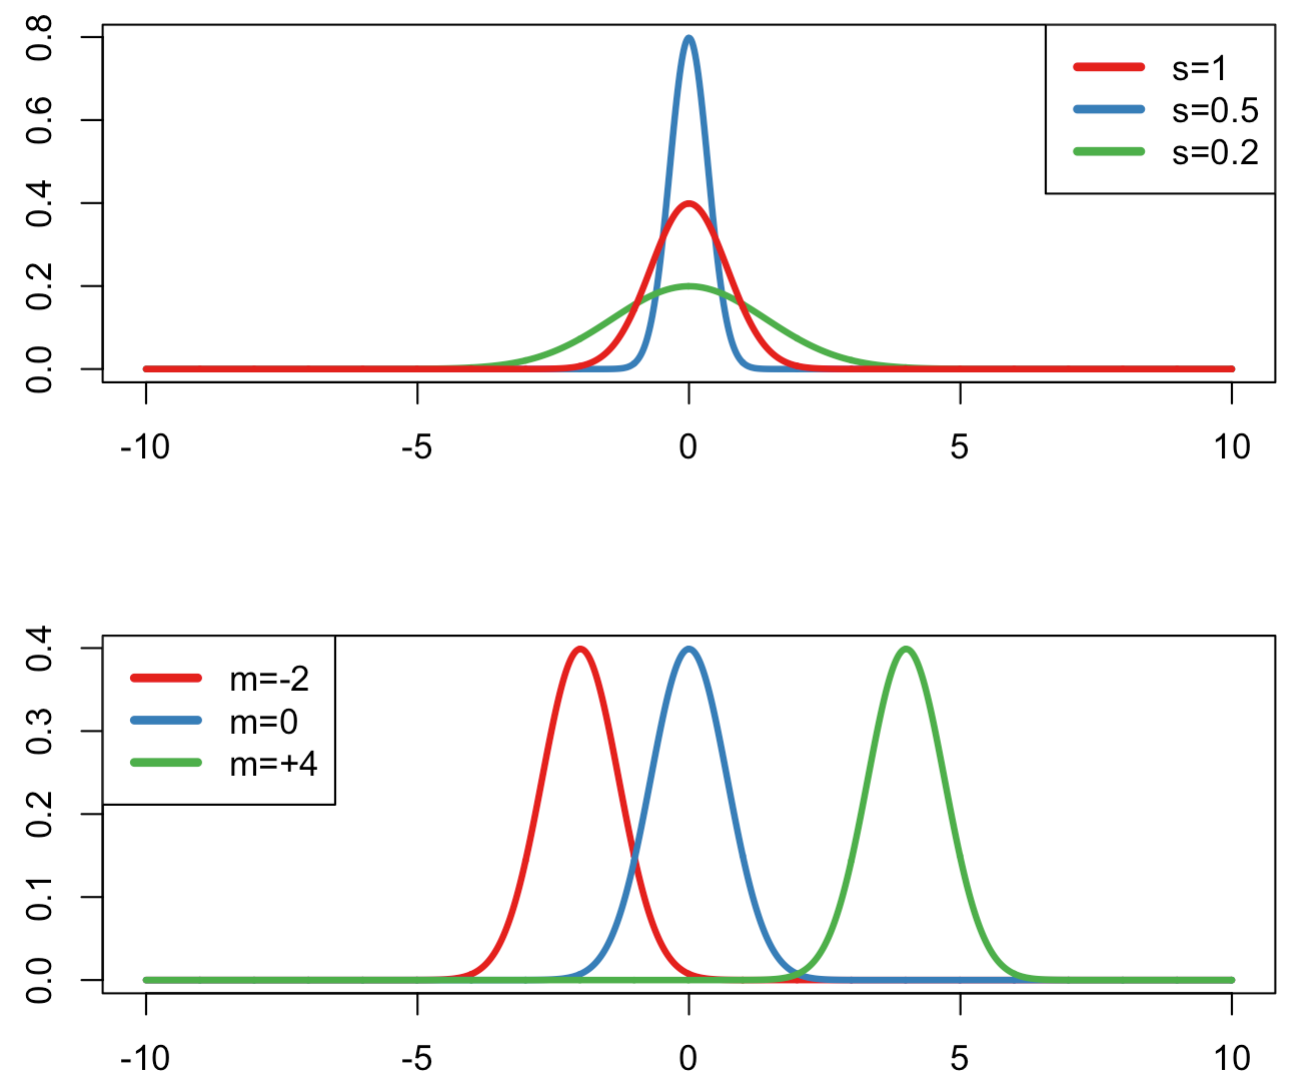
\includegraphics[width=.9\textwidth]{fig/prob10.png}
    \end{center}

\end{frame}


%%%%%%%%%%%%%%%%%%%%%%%%%%%%%%%%%%%%%%%%%%%%%%%%%%%%%
\begin{frame}
    \frametitle{Abschlussfragen}

    \begin{enumerate}
        \item Zeigen Sie, dass der Erwartungswert der Exponential-Verteilung $E(X) = 1/\lambda$ ist.
        \item Zeigen Sie, dass bei der Binomial-Verteilung die Bedingung $\sum_k P(X=k)=1$ erfüllt ist! Benutzen Sie dazu, dass $(a+b)^n = \sum_{k=0}^n \binom{n}{k}a^kb^{n-k}$
        \item Wie groß ist die Wahrscheinlichkeit, dass es unter 100 Personen mindestens eine gibt, die am 10. März Geburtstag hat?
        \item Bestimmen Sie erwartete Anzahl $\lambda$ von Leuten, die in einer Gruppe von 100 am 10. März Geburtstag haben; Bestimmen Sie anhand der Poisson Verteilung $P_{\lambda}(X\ge 1)$ und vergleichen Sie mit der ersten Wahrscheinlichkeit.
        
    \end{enumerate}
    
\end{frame}

%\appendix

\section{Eigenwertaufgaben}
Eigenwerte, Eigenvektoren
Charakteristisches Polynom
Stabilität von Eigenwerten und Eigenvektoren


\end{document}
